% **************************************************************************************************************
% A Classic Thesis Style
% An Homage to The Elements of Typographic Style
%
% Copyright (C) 2012 Andr\'e Miede http://www.miede.de
%
% If you like the style then I would appreciate a postcard. My address 
% can be found in the file ClassicThesis.pdf. A collection of the 
% postcards I received so far is available online at 
% http://postcards.miede.de
%
% License:
% This program is free software; you can redistribute it and/or modify
% it under the terms of the GNU General Public License as published by
% the Free Software Foundation; either version 2 of the License, or
% (at your option) any later version.
%
% This program is distributed in the hope that it will be useful,
% but WITHOUT ANY WARRANTY; without even the implied warranty of
% MERCHANTABILITY or FITNESS FOR A PARTICULAR PURPOSE.  See the
% GNU General Public License for more details.
%
% You should have received a copy of the GNU General Public License
% along with this program; see the file COPYING.  If not, write to
% the Free Software Foundation, Inc., 59 Temple Place - Suite 330,
% Boston, MA 02111-1307, USA.
%
% **************************************************************************************************************
% Note:
%    * You must not use "u etc. in strings/commands that will be spaced out (use \"u or real umlauts instead)
%    * New enumeration (small caps): \begin{aenumerate} \end{aenumerate}
%    * For margin notes: \marginpar or \graffito{}
%    * Do not use bold fonts in this style, it is designed around them
%    * Use tables as in the examples
%    * See classicthesis-preamble.sty for useful commands
% **************************************************************************************************************
% To Do:
%		 * [high] Check this out: http://www.golatex.de/koma-script-warnung-in-verbindung-mit-listings-package-t2058.html
%    * [medium] mathbb in section-titles/chapter-titles => disappears somehow in headlines!!!
% **************************************************************************************************************
\documentclass[ twoside,openright,titlepage,numbers=noenddot,headinclude,%1headlines,% letterpaper a4paper
                footinclude=true,cleardoublepage=empty,abstractoff, % <--- obsolete, remove (todo)
                BCOR=5mm,paper=a4,fontsize=11pt,%11pt,a4paper,%
                ngerman,american,%
                ]{scrreprt}

%********************************************************************
% Note: Make all your adjustments in here
%*******************************************************
% ****************************************************************************************************
% classicthesis-config.tex 
% formerly known as loadpackages.sty, classicthesis-ldpkg.sty, and classicthesis-preamble.sty 
% Use it at the beginning of your ClassicThesis.tex, or as a LaTeX Preamble 
% in your ClassicThesis.{tex,lyx} with % ****************************************************************************************************
% classicthesis-config.tex 
% formerly known as loadpackages.sty, classicthesis-ldpkg.sty, and classicthesis-preamble.sty 
% Use it at the beginning of your ClassicThesis.tex, or as a LaTeX Preamble 
% in your ClassicThesis.{tex,lyx} with % ****************************************************************************************************
% classicthesis-config.tex 
% formerly known as loadpackages.sty, classicthesis-ldpkg.sty, and classicthesis-preamble.sty 
% Use it at the beginning of your ClassicThesis.tex, or as a LaTeX Preamble 
% in your ClassicThesis.{tex,lyx} with \input{classicthesis-config}
% ****************************************************************************************************  
% If you like the classicthesis, then I would appreciate a postcard. 
% My address can be found in the file ClassicThesis.pdf. A collection 
% of the postcards I received so far is available online at 
% http://postcards.miede.de
% ****************************************************************************************************

% ****************************************************************************************************
% 1. Configure classicthesis for your needs here, e.g., remove "drafting" below 
% in order to deactivate the time-stamp on the pages
% ****************************************************************************************************
\PassOptionsToPackage{eulerchapternumbers,listings,drafting,%
				 pdfspacing,%floatperchapter,%linedheaders,%
				 subfig,beramono,eulermath,parts}{classicthesis}										
% ********************************************************************
% Available options for classicthesis.sty 
% (see ClassicThesis.pdf for more information):
% drafting
% parts nochapters linedheaders
% eulerchapternumbers beramono eulermath pdfspacing minionprospacing
% tocaligned dottedtoc manychapters
% listings floatperchapter subfig
% ********************************************************************

% ********************************************************************
% Triggers for this config
% ******************************************************************** 
\usepackage{ifthen}
\newboolean{enable-backrefs} % enable backrefs in the bibliography
\setboolean{enable-backrefs}{false} % true false
% ****************************************************************************************************


% ****************************************************************************************************
% 2. Personal data and user ad-hoc commands
% ****************************************************************************************************
\newcommand{\myTitle}{Non-Native Speech Recognition for Computer Assisted Pronunciation Training\xspace}
\newcommand{\mySubtitle}{The Listener System\xspace}
\newcommand{\myDegree}{MSc\xspace}
\newcommand{\myName}{Gustavo Mendon\c{c}a\xspace}
\newcommand{\myProf}{Sandra Alu\'isio\xspace}
\newcommand{\myOtherProf}{Aldebaro Klautau\xspace}
%\newcommand{\mySupervisor}{Sandra Alu\'isio\xspace}
\newcommand{\myFaculty}{Instituto de Ci\^encias Matem\'aticas e de Computa\c{c}\~ao\xspace}
\newcommand{\myDepartment}{Interinstitutional Center for Computational Linguistics\xspace}
\newcommand{\myUni}{Universidade de S\~ao Paulo\xspace}
\newcommand{\myLocation}{S\~ao Carlos, SP -- Brazil\xspace}
\newcommand{\myTime}{July 2014\xspace}
\newcommand{\myVersion}{version 0.1\xspace}

% ********************************************************************
% Setup, finetuning, and useful commands
% ********************************************************************
\newcounter{dummy} % necessary for correct hyperlinks (to index, bib, etc.)
\newlength{\abcd} % for ab..z string length calculation
\providecommand{\mLyX}{L\kern-.1667em\lower.25em\hbox{Y}\kern-.125emX\@}
\newcommand{\ie}{i.\,e.}
\newcommand{\Ie}{I.\,e.}
\newcommand{\eg}{e.\,g.}
\newcommand{\Eg}{E.\,g.} 
% ****************************************************************************************************


% ****************************************************************************************************
% 3. Loading some handy packages
% ****************************************************************************************************
% ******************************************************************** 
% Packages with options that might require adjustments
% ******************************************************************** 
\PassOptionsToPackage{latin9}{inputenc}	% latin9 (ISO-8859-9) = latin1+"Euro sign"
 \usepackage{inputenc}				

%\PassOptionsToPackage{ngerman,american}{babel}   % change this to your language(s)
% Spanish languages need extra options in order to work with this template
%\PassOptionsToPackage{spanish,es-lcroman}{babel}
 \usepackage{babel}					

\PassOptionsToPackage{square,numbers}{natbib}
 \usepackage{natbib}				
 \usepackage{bibentry}

\PassOptionsToPackage{fleqn}{amsmath}		% math environments and more by the AMS 
 \usepackage{amsmath}

% ******************************************************************** 
% General useful packages
% ******************************************************************** 
\PassOptionsToPackage{T1}{fontenc} % T2A for cyrillics
	\usepackage{fontenc}     
\usepackage{textcomp} % fix warning with missing font shapes
\usepackage{scrhack} % fix warnings when using KOMA with listings package          
\usepackage{xspace} % to get the spacing after macros right  
%\usepackage{mparhack} % get marginpar right
\usepackage{fixltx2e} % fixes some LaTeX stuff 
\PassOptionsToPackage{printonlyused,smaller}{acronym}
	\usepackage{acronym} % nice macros for handling all acronyms in the thesis
%\renewcommand*{\acsfont}[1]{\textssc{#1}} % for MinionPro
\renewcommand{\bflabel}[1]{{#1}\hfill} % fix the list of acronyms
% ****************************************************************************************************


% ****************************************************************************************************
% 4. Setup floats: tables, (sub)figures, and captions
% ****************************************************************************************************
\usepackage{tabularx} % better tables
	\setlength{\extrarowheight}{3pt} % increase table row height
\newcommand{\tableheadline}[1]{\multicolumn{1}{c}{\spacedlowsmallcaps{#1}}}
\newcommand{\myfloatalign}{\centering} % to be used with each float for alignment
\usepackage{caption}
\captionsetup{format=hang,font=small}
\usepackage{subfig}  
% ****************************************************************************************************


% ****************************************************************************************************
% 5. Setup code listings
% ****************************************************************************************************
\usepackage{listings} 
%\lstset{emph={trueIndex,root},emphstyle=\color{BlueViolet}}%\underbar} % for special keywords
\lstset{language=[LaTeX]Tex,%C++,
    keywordstyle=\color{RoyalBlue},%\bfseries,
    basicstyle=\small\ttfamily,
    %identifierstyle=\color{NavyBlue},
    commentstyle=\color{Green}\ttfamily,
    stringstyle=\rmfamily,
    numbers=none,%left,%
    numberstyle=\scriptsize,%\tiny
    stepnumber=5,
    numbersep=8pt,
    showstringspaces=false,
    breaklines=true,
    frameround=ftff,
    frame=single,
    belowcaptionskip=.75\baselineskip
    %frame=L
} 
% ****************************************************************************************************    		   


% ****************************************************************************************************
% 6. PDFLaTeX, hyperreferences and citation backreferences
% ****************************************************************************************************
% ********************************************************************
% Using PDFLaTeX
% ********************************************************************
\PassOptionsToPackage{pdftex,hyperfootnotes=false,pdfpagelabels}{hyperref}
	\usepackage{hyperref}  % backref linktocpage pagebackref
\pdfcompresslevel=9
\pdfadjustspacing=1 
\PassOptionsToPackage{pdftex}{graphicx}
	\usepackage{graphicx} 

% ********************************************************************
% Setup the style of the backrefs from the bibliography
% (translate the options to any language you use)
% ********************************************************************
\newcommand{\backrefnotcitedstring}{\relax}%(Not cited.)
\newcommand{\backrefcitedsinglestring}[1]{(Cited on page~#1.)}
\newcommand{\backrefcitedmultistring}[1]{(Cited on pages~#1.)}
\ifthenelse{\boolean{enable-backrefs}}%
{%
		\PassOptionsToPackage{hyperpageref}{backref}
		\usepackage{backref} % to be loaded after hyperref package 
		   \renewcommand{\backreftwosep}{ and~} % separate 2 pages
		   \renewcommand{\backreflastsep}{, and~} % separate last of longer list
		   \renewcommand*{\backref}[1]{}  % disable standard
		   \renewcommand*{\backrefalt}[4]{% detailed backref
		      \ifcase #1 %
		         \backrefnotcitedstring%
		      \or%
		         \backrefcitedsinglestring{#2}%
		      \else%
		         \backrefcitedmultistring{#2}%
		      \fi}%
}{\relax}    

% ********************************************************************
% Hyperreferences
% ********************************************************************
\hypersetup{%
    %draft,	% = no hyperlinking at all (useful in b/w printouts)
    colorlinks=true, linktocpage=true, pdfstartpage=3, pdfstartview=FitV,%
    % uncomment the following line if you want to have black links (e.g., for printing)
    %colorlinks=false, linktocpage=false, pdfborder={0 0 0}, pdfstartpage=3, pdfstartview=FitV,% 
    breaklinks=true, pdfpagemode=UseNone, pageanchor=true, pdfpagemode=UseOutlines,%
    plainpages=false, bookmarksnumbered, bookmarksopen=true, bookmarksopenlevel=1,%
    hypertexnames=true, pdfhighlight=/O,%nesting=true,%frenchlinks,%
    urlcolor=webbrown, linkcolor=black, citecolor=black, %pagecolor=RoyalBlue,%
    %urlcolor=Black, linkcolor=Black, citecolor=Black, %pagecolor=Black,%
    pdftitle={\myTitle},%
    pdfauthor={\textcopyright\ \myName, \myUni, \myFaculty},%
    pdfsubject={},%
    pdfkeywords={},%
    pdfcreator={pdfLaTeX},%
    pdfproducer={LaTeX with hyperref and classicthesis}%
}   

% ********************************************************************
% Setup autoreferences
% ********************************************************************
% There are some issues regarding autorefnames
% http://www.ureader.de/msg/136221647.aspx
% http://www.tex.ac.uk/cgi-bin/texfaq2html?label=latexwords
% you have to redefine the makros for the 
% language you use, e.g., american, ngerman
% (as chosen when loading babel/AtBeginDocument)
% ********************************************************************
\makeatletter
\@ifpackageloaded{babel}%
    {%
       \addto\extrasamerican{%
					\renewcommand*{\figureautorefname}{Figure}%
					\renewcommand*{\tableautorefname}{Table}%
					\renewcommand*{\partautorefname}{Part}%
					\renewcommand*{\chapterautorefname}{Chapter}%
					\renewcommand*{\sectionautorefname}{Section}%
					\renewcommand*{\subsectionautorefname}{Section}%
					\renewcommand*{\subsubsectionautorefname}{Section}% 	
				}%
       \addto\extrasngerman{% 
					\renewcommand*{\paragraphautorefname}{Absatz}%
					\renewcommand*{\subparagraphautorefname}{Unterabsatz}%
					\renewcommand*{\footnoteautorefname}{Fu\"snote}%
					\renewcommand*{\FancyVerbLineautorefname}{Zeile}%
					\renewcommand*{\theoremautorefname}{Theorem}%
					\renewcommand*{\appendixautorefname}{Anhang}%
					\renewcommand*{\equationautorefname}{Gleichung}%        
					\renewcommand*{\itemautorefname}{Punkt}%
				}%	
			% Fix to getting autorefs for subfigures right (thanks to Belinda Vogt for changing the definition)
			\providecommand{\subfigureautorefname}{\figureautorefname}%  			
    }{\relax}
\makeatother


% ****************************************************************************************************
% 7. Last calls before the bar closes
% ****************************************************************************************************
% ********************************************************************
% Development Stuff
% ********************************************************************
\listfiles
%\PassOptionsToPackage{l2tabu,orthodox,abort}{nag}
%	\usepackage{nag}
%\PassOptionsToPackage{warning, all}{onlyamsmath}
%	\usepackage{onlyamsmath}

% ********************************************************************
% Last, but not least...
% ********************************************************************
\usepackage{classicthesis} 
% ****************************************************************************************************


% ****************************************************************************************************
% 8. Further adjustments (experimental)
% ****************************************************************************************************
% ********************************************************************
% Changing the text area
% ********************************************************************
%\linespread{1.05} % a bit more for Palatino
%\areaset[current]{312pt}{761pt} % 686 (factor 2.2) + 33 head + 42 head \the\footskip
%\setlength{\marginparwidth}{7em}%
%\setlength{\marginparsep}{2em}%

% ********************************************************************
% Using different fonts
% ********************************************************************
%\usepackage[oldstylenums]{kpfonts} % oldstyle notextcomp
%\usepackage[osf]{libertine}
%\usepackage{hfoldsty} % Computer Modern with osf
%\usepackage[light,condensed,math]{iwona}
%\renewcommand{\sfdefault}{iwona}
%\usepackage{lmodern} % <-- no osf support :-(
%\usepackage[urw-garamond]{mathdesign} <-- no osf support :-(
% ****************************************************************************************************

% ****************************************************************************************************  
% If you like the classicthesis, then I would appreciate a postcard. 
% My address can be found in the file ClassicThesis.pdf. A collection 
% of the postcards I received so far is available online at 
% http://postcards.miede.de
% ****************************************************************************************************

% ****************************************************************************************************
% 1. Configure classicthesis for your needs here, e.g., remove "drafting" below 
% in order to deactivate the time-stamp on the pages
% ****************************************************************************************************
\PassOptionsToPackage{eulerchapternumbers,listings,drafting,%
				 pdfspacing,%floatperchapter,%linedheaders,%
				 subfig,beramono,eulermath,parts}{classicthesis}										
% ********************************************************************
% Available options for classicthesis.sty 
% (see ClassicThesis.pdf for more information):
% drafting
% parts nochapters linedheaders
% eulerchapternumbers beramono eulermath pdfspacing minionprospacing
% tocaligned dottedtoc manychapters
% listings floatperchapter subfig
% ********************************************************************

% ********************************************************************
% Triggers for this config
% ******************************************************************** 
\usepackage{ifthen}
\newboolean{enable-backrefs} % enable backrefs in the bibliography
\setboolean{enable-backrefs}{false} % true false
% ****************************************************************************************************


% ****************************************************************************************************
% 2. Personal data and user ad-hoc commands
% ****************************************************************************************************
\newcommand{\myTitle}{Non-Native Speech Recognition for Computer Assisted Pronunciation Training\xspace}
\newcommand{\mySubtitle}{The Listener System\xspace}
\newcommand{\myDegree}{MSc\xspace}
\newcommand{\myName}{Gustavo Mendon\c{c}a\xspace}
\newcommand{\myProf}{Sandra Alu\'isio\xspace}
\newcommand{\myOtherProf}{Aldebaro Klautau\xspace}
%\newcommand{\mySupervisor}{Sandra Alu\'isio\xspace}
\newcommand{\myFaculty}{Instituto de Ci\^encias Matem\'aticas e de Computa\c{c}\~ao\xspace}
\newcommand{\myDepartment}{Interinstitutional Center for Computational Linguistics\xspace}
\newcommand{\myUni}{Universidade de S\~ao Paulo\xspace}
\newcommand{\myLocation}{S\~ao Carlos, SP -- Brazil\xspace}
\newcommand{\myTime}{July 2014\xspace}
\newcommand{\myVersion}{version 0.1\xspace}

% ********************************************************************
% Setup, finetuning, and useful commands
% ********************************************************************
\newcounter{dummy} % necessary for correct hyperlinks (to index, bib, etc.)
\newlength{\abcd} % for ab..z string length calculation
\providecommand{\mLyX}{L\kern-.1667em\lower.25em\hbox{Y}\kern-.125emX\@}
\newcommand{\ie}{i.\,e.}
\newcommand{\Ie}{I.\,e.}
\newcommand{\eg}{e.\,g.}
\newcommand{\Eg}{E.\,g.} 
% ****************************************************************************************************


% ****************************************************************************************************
% 3. Loading some handy packages
% ****************************************************************************************************
% ******************************************************************** 
% Packages with options that might require adjustments
% ******************************************************************** 
\PassOptionsToPackage{latin9}{inputenc}	% latin9 (ISO-8859-9) = latin1+"Euro sign"
 \usepackage{inputenc}				

%\PassOptionsToPackage{ngerman,american}{babel}   % change this to your language(s)
% Spanish languages need extra options in order to work with this template
%\PassOptionsToPackage{spanish,es-lcroman}{babel}
 \usepackage{babel}					

\PassOptionsToPackage{square,numbers}{natbib}
 \usepackage{natbib}				
 \usepackage{bibentry}

\PassOptionsToPackage{fleqn}{amsmath}		% math environments and more by the AMS 
 \usepackage{amsmath}

% ******************************************************************** 
% General useful packages
% ******************************************************************** 
\PassOptionsToPackage{T1}{fontenc} % T2A for cyrillics
	\usepackage{fontenc}     
\usepackage{textcomp} % fix warning with missing font shapes
\usepackage{scrhack} % fix warnings when using KOMA with listings package          
\usepackage{xspace} % to get the spacing after macros right  
%\usepackage{mparhack} % get marginpar right
\usepackage{fixltx2e} % fixes some LaTeX stuff 
\PassOptionsToPackage{printonlyused,smaller}{acronym}
	\usepackage{acronym} % nice macros for handling all acronyms in the thesis
%\renewcommand*{\acsfont}[1]{\textssc{#1}} % for MinionPro
\renewcommand{\bflabel}[1]{{#1}\hfill} % fix the list of acronyms
% ****************************************************************************************************


% ****************************************************************************************************
% 4. Setup floats: tables, (sub)figures, and captions
% ****************************************************************************************************
\usepackage{tabularx} % better tables
	\setlength{\extrarowheight}{3pt} % increase table row height
\newcommand{\tableheadline}[1]{\multicolumn{1}{c}{\spacedlowsmallcaps{#1}}}
\newcommand{\myfloatalign}{\centering} % to be used with each float for alignment
\usepackage{caption}
\captionsetup{format=hang,font=small}
\usepackage{subfig}  
% ****************************************************************************************************


% ****************************************************************************************************
% 5. Setup code listings
% ****************************************************************************************************
\usepackage{listings} 
%\lstset{emph={trueIndex,root},emphstyle=\color{BlueViolet}}%\underbar} % for special keywords
\lstset{language=[LaTeX]Tex,%C++,
    keywordstyle=\color{RoyalBlue},%\bfseries,
    basicstyle=\small\ttfamily,
    %identifierstyle=\color{NavyBlue},
    commentstyle=\color{Green}\ttfamily,
    stringstyle=\rmfamily,
    numbers=none,%left,%
    numberstyle=\scriptsize,%\tiny
    stepnumber=5,
    numbersep=8pt,
    showstringspaces=false,
    breaklines=true,
    frameround=ftff,
    frame=single,
    belowcaptionskip=.75\baselineskip
    %frame=L
} 
% ****************************************************************************************************    		   


% ****************************************************************************************************
% 6. PDFLaTeX, hyperreferences and citation backreferences
% ****************************************************************************************************
% ********************************************************************
% Using PDFLaTeX
% ********************************************************************
\PassOptionsToPackage{pdftex,hyperfootnotes=false,pdfpagelabels}{hyperref}
	\usepackage{hyperref}  % backref linktocpage pagebackref
\pdfcompresslevel=9
\pdfadjustspacing=1 
\PassOptionsToPackage{pdftex}{graphicx}
	\usepackage{graphicx} 

% ********************************************************************
% Setup the style of the backrefs from the bibliography
% (translate the options to any language you use)
% ********************************************************************
\newcommand{\backrefnotcitedstring}{\relax}%(Not cited.)
\newcommand{\backrefcitedsinglestring}[1]{(Cited on page~#1.)}
\newcommand{\backrefcitedmultistring}[1]{(Cited on pages~#1.)}
\ifthenelse{\boolean{enable-backrefs}}%
{%
		\PassOptionsToPackage{hyperpageref}{backref}
		\usepackage{backref} % to be loaded after hyperref package 
		   \renewcommand{\backreftwosep}{ and~} % separate 2 pages
		   \renewcommand{\backreflastsep}{, and~} % separate last of longer list
		   \renewcommand*{\backref}[1]{}  % disable standard
		   \renewcommand*{\backrefalt}[4]{% detailed backref
		      \ifcase #1 %
		         \backrefnotcitedstring%
		      \or%
		         \backrefcitedsinglestring{#2}%
		      \else%
		         \backrefcitedmultistring{#2}%
		      \fi}%
}{\relax}    

% ********************************************************************
% Hyperreferences
% ********************************************************************
\hypersetup{%
    %draft,	% = no hyperlinking at all (useful in b/w printouts)
    colorlinks=true, linktocpage=true, pdfstartpage=3, pdfstartview=FitV,%
    % uncomment the following line if you want to have black links (e.g., for printing)
    %colorlinks=false, linktocpage=false, pdfborder={0 0 0}, pdfstartpage=3, pdfstartview=FitV,% 
    breaklinks=true, pdfpagemode=UseNone, pageanchor=true, pdfpagemode=UseOutlines,%
    plainpages=false, bookmarksnumbered, bookmarksopen=true, bookmarksopenlevel=1,%
    hypertexnames=true, pdfhighlight=/O,%nesting=true,%frenchlinks,%
    urlcolor=webbrown, linkcolor=black, citecolor=black, %pagecolor=RoyalBlue,%
    %urlcolor=Black, linkcolor=Black, citecolor=Black, %pagecolor=Black,%
    pdftitle={\myTitle},%
    pdfauthor={\textcopyright\ \myName, \myUni, \myFaculty},%
    pdfsubject={},%
    pdfkeywords={},%
    pdfcreator={pdfLaTeX},%
    pdfproducer={LaTeX with hyperref and classicthesis}%
}   

% ********************************************************************
% Setup autoreferences
% ********************************************************************
% There are some issues regarding autorefnames
% http://www.ureader.de/msg/136221647.aspx
% http://www.tex.ac.uk/cgi-bin/texfaq2html?label=latexwords
% you have to redefine the makros for the 
% language you use, e.g., american, ngerman
% (as chosen when loading babel/AtBeginDocument)
% ********************************************************************
\makeatletter
\@ifpackageloaded{babel}%
    {%
       \addto\extrasamerican{%
					\renewcommand*{\figureautorefname}{Figure}%
					\renewcommand*{\tableautorefname}{Table}%
					\renewcommand*{\partautorefname}{Part}%
					\renewcommand*{\chapterautorefname}{Chapter}%
					\renewcommand*{\sectionautorefname}{Section}%
					\renewcommand*{\subsectionautorefname}{Section}%
					\renewcommand*{\subsubsectionautorefname}{Section}% 	
				}%
       \addto\extrasngerman{% 
					\renewcommand*{\paragraphautorefname}{Absatz}%
					\renewcommand*{\subparagraphautorefname}{Unterabsatz}%
					\renewcommand*{\footnoteautorefname}{Fu\"snote}%
					\renewcommand*{\FancyVerbLineautorefname}{Zeile}%
					\renewcommand*{\theoremautorefname}{Theorem}%
					\renewcommand*{\appendixautorefname}{Anhang}%
					\renewcommand*{\equationautorefname}{Gleichung}%        
					\renewcommand*{\itemautorefname}{Punkt}%
				}%	
			% Fix to getting autorefs for subfigures right (thanks to Belinda Vogt for changing the definition)
			\providecommand{\subfigureautorefname}{\figureautorefname}%  			
    }{\relax}
\makeatother


% ****************************************************************************************************
% 7. Last calls before the bar closes
% ****************************************************************************************************
% ********************************************************************
% Development Stuff
% ********************************************************************
\listfiles
%\PassOptionsToPackage{l2tabu,orthodox,abort}{nag}
%	\usepackage{nag}
%\PassOptionsToPackage{warning, all}{onlyamsmath}
%	\usepackage{onlyamsmath}

% ********************************************************************
% Last, but not least...
% ********************************************************************
\usepackage{classicthesis} 
% ****************************************************************************************************


% ****************************************************************************************************
% 8. Further adjustments (experimental)
% ****************************************************************************************************
% ********************************************************************
% Changing the text area
% ********************************************************************
%\linespread{1.05} % a bit more for Palatino
%\areaset[current]{312pt}{761pt} % 686 (factor 2.2) + 33 head + 42 head \the\footskip
%\setlength{\marginparwidth}{7em}%
%\setlength{\marginparsep}{2em}%

% ********************************************************************
% Using different fonts
% ********************************************************************
%\usepackage[oldstylenums]{kpfonts} % oldstyle notextcomp
%\usepackage[osf]{libertine}
%\usepackage{hfoldsty} % Computer Modern with osf
%\usepackage[light,condensed,math]{iwona}
%\renewcommand{\sfdefault}{iwona}
%\usepackage{lmodern} % <-- no osf support :-(
%\usepackage[urw-garamond]{mathdesign} <-- no osf support :-(
% ****************************************************************************************************

% ****************************************************************************************************  
% If you like the classicthesis, then I would appreciate a postcard. 
% My address can be found in the file ClassicThesis.pdf. A collection 
% of the postcards I received so far is available online at 
% http://postcards.miede.de
% ****************************************************************************************************

% ****************************************************************************************************
% 1. Configure classicthesis for your needs here, e.g., remove "drafting" below 
% in order to deactivate the time-stamp on the pages
% ****************************************************************************************************
\PassOptionsToPackage{eulerchapternumbers,listings,drafting,%
				 pdfspacing,%floatperchapter,%linedheaders,%
				 subfig,beramono,eulermath,parts}{classicthesis}										
% ********************************************************************
% Available options for classicthesis.sty 
% (see ClassicThesis.pdf for more information):
% drafting
% parts nochapters linedheaders
% eulerchapternumbers beramono eulermath pdfspacing minionprospacing
% tocaligned dottedtoc manychapters
% listings floatperchapter subfig
% ********************************************************************

% ********************************************************************
% Triggers for this config
% ******************************************************************** 
\usepackage{ifthen}
\newboolean{enable-backrefs} % enable backrefs in the bibliography
\setboolean{enable-backrefs}{false} % true false
% ****************************************************************************************************


% ****************************************************************************************************
% 2. Personal data and user ad-hoc commands
% ****************************************************************************************************
\newcommand{\myTitle}{Non-Native Speech Recognition for Computer Assisted Pronunciation Training\xspace}
\newcommand{\mySubtitle}{The Listener System\xspace}
\newcommand{\myDegree}{MSc\xspace}
\newcommand{\myName}{Gustavo Mendon\c{c}a\xspace}
\newcommand{\myProf}{Sandra Alu\'isio\xspace}
\newcommand{\myOtherProf}{Aldebaro Klautau\xspace}
%\newcommand{\mySupervisor}{Sandra Alu\'isio\xspace}
\newcommand{\myFaculty}{Instituto de Ci\^encias Matem\'aticas e de Computa\c{c}\~ao\xspace}
\newcommand{\myDepartment}{Interinstitutional Center for Computational Linguistics\xspace}
\newcommand{\myUni}{Universidade de S\~ao Paulo\xspace}
\newcommand{\myLocation}{S\~ao Carlos, SP -- Brazil\xspace}
\newcommand{\myTime}{July 2014\xspace}
\newcommand{\myVersion}{version 0.1\xspace}

% ********************************************************************
% Setup, finetuning, and useful commands
% ********************************************************************
\newcounter{dummy} % necessary for correct hyperlinks (to index, bib, etc.)
\newlength{\abcd} % for ab..z string length calculation
\providecommand{\mLyX}{L\kern-.1667em\lower.25em\hbox{Y}\kern-.125emX\@}
\newcommand{\ie}{i.\,e.}
\newcommand{\Ie}{I.\,e.}
\newcommand{\eg}{e.\,g.}
\newcommand{\Eg}{E.\,g.} 
% ****************************************************************************************************


% ****************************************************************************************************
% 3. Loading some handy packages
% ****************************************************************************************************
% ******************************************************************** 
% Packages with options that might require adjustments
% ******************************************************************** 
\PassOptionsToPackage{latin9}{inputenc}	% latin9 (ISO-8859-9) = latin1+"Euro sign"
 \usepackage{inputenc}				

%\PassOptionsToPackage{ngerman,american}{babel}   % change this to your language(s)
% Spanish languages need extra options in order to work with this template
%\PassOptionsToPackage{spanish,es-lcroman}{babel}
 \usepackage{babel}					

\PassOptionsToPackage{square,numbers}{natbib}
 \usepackage{natbib}				
 \usepackage{bibentry}

\PassOptionsToPackage{fleqn}{amsmath}		% math environments and more by the AMS 
 \usepackage{amsmath}

% ******************************************************************** 
% General useful packages
% ******************************************************************** 
\PassOptionsToPackage{T1}{fontenc} % T2A for cyrillics
	\usepackage{fontenc}     
\usepackage{textcomp} % fix warning with missing font shapes
\usepackage{scrhack} % fix warnings when using KOMA with listings package          
\usepackage{xspace} % to get the spacing after macros right  
%\usepackage{mparhack} % get marginpar right
\usepackage{fixltx2e} % fixes some LaTeX stuff 
\PassOptionsToPackage{printonlyused,smaller}{acronym}
	\usepackage{acronym} % nice macros for handling all acronyms in the thesis
%\renewcommand*{\acsfont}[1]{\textssc{#1}} % for MinionPro
\renewcommand{\bflabel}[1]{{#1}\hfill} % fix the list of acronyms
% ****************************************************************************************************


% ****************************************************************************************************
% 4. Setup floats: tables, (sub)figures, and captions
% ****************************************************************************************************
\usepackage{tabularx} % better tables
	\setlength{\extrarowheight}{3pt} % increase table row height
\newcommand{\tableheadline}[1]{\multicolumn{1}{c}{\spacedlowsmallcaps{#1}}}
\newcommand{\myfloatalign}{\centering} % to be used with each float for alignment
\usepackage{caption}
\captionsetup{format=hang,font=small}
\usepackage{subfig}  
% ****************************************************************************************************


% ****************************************************************************************************
% 5. Setup code listings
% ****************************************************************************************************
\usepackage{listings} 
%\lstset{emph={trueIndex,root},emphstyle=\color{BlueViolet}}%\underbar} % for special keywords
\lstset{language=[LaTeX]Tex,%C++,
    keywordstyle=\color{RoyalBlue},%\bfseries,
    basicstyle=\small\ttfamily,
    %identifierstyle=\color{NavyBlue},
    commentstyle=\color{Green}\ttfamily,
    stringstyle=\rmfamily,
    numbers=none,%left,%
    numberstyle=\scriptsize,%\tiny
    stepnumber=5,
    numbersep=8pt,
    showstringspaces=false,
    breaklines=true,
    frameround=ftff,
    frame=single,
    belowcaptionskip=.75\baselineskip
    %frame=L
} 
% ****************************************************************************************************    		   


% ****************************************************************************************************
% 6. PDFLaTeX, hyperreferences and citation backreferences
% ****************************************************************************************************
% ********************************************************************
% Using PDFLaTeX
% ********************************************************************
\PassOptionsToPackage{pdftex,hyperfootnotes=false,pdfpagelabels}{hyperref}
	\usepackage{hyperref}  % backref linktocpage pagebackref
\pdfcompresslevel=9
\pdfadjustspacing=1 
\PassOptionsToPackage{pdftex}{graphicx}
	\usepackage{graphicx} 

% ********************************************************************
% Setup the style of the backrefs from the bibliography
% (translate the options to any language you use)
% ********************************************************************
\newcommand{\backrefnotcitedstring}{\relax}%(Not cited.)
\newcommand{\backrefcitedsinglestring}[1]{(Cited on page~#1.)}
\newcommand{\backrefcitedmultistring}[1]{(Cited on pages~#1.)}
\ifthenelse{\boolean{enable-backrefs}}%
{%
		\PassOptionsToPackage{hyperpageref}{backref}
		\usepackage{backref} % to be loaded after hyperref package 
		   \renewcommand{\backreftwosep}{ and~} % separate 2 pages
		   \renewcommand{\backreflastsep}{, and~} % separate last of longer list
		   \renewcommand*{\backref}[1]{}  % disable standard
		   \renewcommand*{\backrefalt}[4]{% detailed backref
		      \ifcase #1 %
		         \backrefnotcitedstring%
		      \or%
		         \backrefcitedsinglestring{#2}%
		      \else%
		         \backrefcitedmultistring{#2}%
		      \fi}%
}{\relax}    

% ********************************************************************
% Hyperreferences
% ********************************************************************
\hypersetup{%
    %draft,	% = no hyperlinking at all (useful in b/w printouts)
    colorlinks=true, linktocpage=true, pdfstartpage=3, pdfstartview=FitV,%
    % uncomment the following line if you want to have black links (e.g., for printing)
    %colorlinks=false, linktocpage=false, pdfborder={0 0 0}, pdfstartpage=3, pdfstartview=FitV,% 
    breaklinks=true, pdfpagemode=UseNone, pageanchor=true, pdfpagemode=UseOutlines,%
    plainpages=false, bookmarksnumbered, bookmarksopen=true, bookmarksopenlevel=1,%
    hypertexnames=true, pdfhighlight=/O,%nesting=true,%frenchlinks,%
    urlcolor=webbrown, linkcolor=black, citecolor=black, %pagecolor=RoyalBlue,%
    %urlcolor=Black, linkcolor=Black, citecolor=Black, %pagecolor=Black,%
    pdftitle={\myTitle},%
    pdfauthor={\textcopyright\ \myName, \myUni, \myFaculty},%
    pdfsubject={},%
    pdfkeywords={},%
    pdfcreator={pdfLaTeX},%
    pdfproducer={LaTeX with hyperref and classicthesis}%
}   

% ********************************************************************
% Setup autoreferences
% ********************************************************************
% There are some issues regarding autorefnames
% http://www.ureader.de/msg/136221647.aspx
% http://www.tex.ac.uk/cgi-bin/texfaq2html?label=latexwords
% you have to redefine the makros for the 
% language you use, e.g., american, ngerman
% (as chosen when loading babel/AtBeginDocument)
% ********************************************************************
\makeatletter
\@ifpackageloaded{babel}%
    {%
       \addto\extrasamerican{%
					\renewcommand*{\figureautorefname}{Figure}%
					\renewcommand*{\tableautorefname}{Table}%
					\renewcommand*{\partautorefname}{Part}%
					\renewcommand*{\chapterautorefname}{Chapter}%
					\renewcommand*{\sectionautorefname}{Section}%
					\renewcommand*{\subsectionautorefname}{Section}%
					\renewcommand*{\subsubsectionautorefname}{Section}% 	
				}%
       \addto\extrasngerman{% 
					\renewcommand*{\paragraphautorefname}{Absatz}%
					\renewcommand*{\subparagraphautorefname}{Unterabsatz}%
					\renewcommand*{\footnoteautorefname}{Fu\"snote}%
					\renewcommand*{\FancyVerbLineautorefname}{Zeile}%
					\renewcommand*{\theoremautorefname}{Theorem}%
					\renewcommand*{\appendixautorefname}{Anhang}%
					\renewcommand*{\equationautorefname}{Gleichung}%        
					\renewcommand*{\itemautorefname}{Punkt}%
				}%	
			% Fix to getting autorefs for subfigures right (thanks to Belinda Vogt for changing the definition)
			\providecommand{\subfigureautorefname}{\figureautorefname}%  			
    }{\relax}
\makeatother


% ****************************************************************************************************
% 7. Last calls before the bar closes
% ****************************************************************************************************
% ********************************************************************
% Development Stuff
% ********************************************************************
\listfiles
%\PassOptionsToPackage{l2tabu,orthodox,abort}{nag}
%	\usepackage{nag}
%\PassOptionsToPackage{warning, all}{onlyamsmath}
%	\usepackage{onlyamsmath}

% ********************************************************************
% Last, but not least...
% ********************************************************************
\usepackage{classicthesis} 
% ****************************************************************************************************


% ****************************************************************************************************
% 8. Further adjustments (experimental)
% ****************************************************************************************************
% ********************************************************************
% Changing the text area
% ********************************************************************
%\linespread{1.05} % a bit more for Palatino
%\areaset[current]{312pt}{761pt} % 686 (factor 2.2) + 33 head + 42 head \the\footskip
%\setlength{\marginparwidth}{7em}%
%\setlength{\marginparsep}{2em}%

% ********************************************************************
% Using different fonts
% ********************************************************************
%\usepackage[oldstylenums]{kpfonts} % oldstyle notextcomp
%\usepackage[osf]{libertine}
%\usepackage{hfoldsty} % Computer Modern with osf
%\usepackage[light,condensed,math]{iwona}
%\renewcommand{\sfdefault}{iwona}
%\usepackage{lmodern} % <-- no osf support :-(
%\usepackage[urw-garamond]{mathdesign} <-- no osf support :-(
% ****************************************************************************************************

\usepackage{tipa}
\usepackage{multicol}
\usepackage{multirow}
\usepackage{lingmacros}
\usepackage{tabularx}
\usepackage{nameref}

\newcommand{\gustavo}[1]{\textbf{#1}}
%********************************************************************
% Hyphenation
%*******************************************************
%\hyphenation{put special hyphenation here}

% ********************************************************************
% GO!GO!GO! MOVE IT!
%*******************************************************
\begin{document}
\frenchspacing
\raggedbottom
\selectlanguage{american} % american ngerman
%\renewcommand*{\bibname}{new name}
%\setbibpreamble{}
\pagenumbering{roman}
\pagestyle{plain}
%********************************************************************
% Frontmatter
%*******************************************************

%*******************************************************
% Little Dirty Titlepage
%*******************************************************
\thispagestyle{empty}
%\pdfbookmark[1]{Titel}{title}
%*******************************************************
\begin{center}
    \spacedlowsmallcaps{\myName} \\ \medskip                        

    \begingroup
        \color{Maroon}\spacedallcaps{\myTitle}
    \endgroup
\end{center}        

%*******************************************************
% Titlepage
%*******************************************************
\begin{titlepage}
	% if you want the titlepage to be centered, uncomment and fine-tune the line below (KOMA classes environment)
	\begin{addmargin}[-1cm]{-3cm}
    \begin{center}
        \large  

        \hfill

        \vfill

        \begingroup
            \color{Maroon}\spacedallcaps{\myTitle}: \\
            \spacedallcaps{\mySubtitle} \bigskip
        \endgroup

        \spacedlowsmallcaps{\myName}

        \vfill

        
\includegraphics[width=6cm]{./gfx/listener_logo.pdf} \\ \medskip

        \vfill 
        
	\myFaculty \\
	\myUni \\
	\myLocation \\  

        \myTime\ -- \myVersion

                             

    \end{center}  
  \end{addmargin}       
\end{titlepage}   
\thispagestyle{empty}

\hfill

\vfill

\noindent\myName: \textit{\myTitle,} \mySubtitle

\bigskip
%
\noindent\spacedlowsmallcaps{Supervisors}: \\
\myProf \\
\myOtherProf \\ 

%
\medskip
%
\noindent\spacedlowsmallcaps{Location}: \\
\myLocation \\
%
\medskip
%
\noindent\spacedlowsmallcaps{Time Frame}: \\
\myTime

%*******************************************************
% Dedication
%*******************************************************
\thispagestyle{empty}
%\phantomsection 
\refstepcounter{dummy}
\pdfbookmark[1]{Dedication}{Dedication}

\vspace*{3cm}

\begin{center}
    To the loving memory of my father, \\ \smallskip
    \emph{Tarc\'izio Ot\'avio Almeida}. \\ \medskip
    1947\,--\,2003
\end{center}

\begin{figure}[!htb]
        \myfloatalign
        {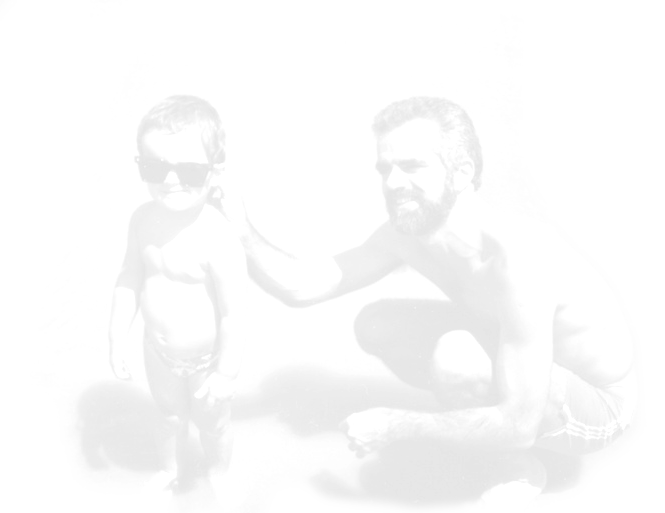
\includegraphics[width=.66\linewidth]{gfx/dad.png}}
\end{figure}
%\cleardoublepage\include{FrontBackmatter/Foreword}
%*******************************************************
% Abstract
%*******************************************************
%\renewcommand{\abstractname}{Abstract}
\pdfbookmark[1]{Abstract}{Abstract}
\begingroup
\let\clearpage\relax
\let\cleardoublepage\relax
\let\cleardoublepage\relax

\chapter*{Abstract}

Pesquisas recentes t\^em avaliado o Brasil entre os pa\'ises com menor n\'ivel
de profici\^encia em l\'ingua inglesa. Este projeto busca criar um recurso
que possa contribuir para a melhoria desse cen\'ario. O objetivo \'e
desenvolver um reconhecedor de pron\'uncia para falantes do portugu\^es
brasileiro (PB) aprendizes de ingl\^es, chamado Listener, que seja capaz
de fornecer ao usu\'ario feedback sobre sua pron\'uncia. Recursos
semelhantes j\'a foram desenvolvidos para outras l\'inguas, no entanto, para
o PB, h\'a ainda uma lacuna a ser explorada. A hip\'otese de pesquisa \'e que
\'e poss\'ivel construir tal reconhecedor de pron\'uncia atrav\'es de: (i) uma
classifica\c{c}\~ao de erros de pron\'uncia que leve em conta a transfer\^encia de
padr\~oes de L1 para L2; (ii) um modelo ac\'ustico que agregue dados de fala
do ingl\^es tanto de nativos, quanto de aprendizes; (iii) um dicion\'ario de
pron\'uncia que contenha a transcri\c{c}\~ao das pron\'uncias desviantes do
aprendiz; e (iv) um modelo de l\'ingua que condiga com a sintaxe do
aprendiz. Nove erros de pron\'uncia foram selecionados para serem tratados
pelo Listener, assumindo-se, como pron\'uncia padr\~ao, o General American
(GA). A engine Julius ser\'a empregada como base do reconhecedor. O modelo
ac\'ustico ser\'a compilado a partir de um corpus de fala de nativos de
ingl\^es: TIMIT Acoustic-Phonetic Continuous Speech Corpus{[}1{]}; e outro
de aprendizes: COBAI - Corpus Oral Brasileiro de Aprendizes de
Ingl\^es{[}2{]}. O dicion\'ario a ser empregado \'e o CMU Pronouncing
Dictionary, ao qual ser\~ao acrescentaremos as hip\'oteses de pron\'uncia dos
aprendizes, por meio de regras. O modelo de l\'ingua ser\'a gerado a partir
da Simple English Wikipedia em conjunto com um corpus de textos escritos
por aprendizes de ingl\^es, o COMAprend{[}3{]}, um dos tr\^es corpus do
projeto COMET da Faculdade de Filosofia, Letras e Ci\^encias Humanas da
Universidade de S\~ao Paulo. A efici\^encia do reconhecedor ser\'a avaliada
por meio de medidas de Word Error Rate (WER), Character Error Rate (CER)
e matrizes de confus\~ao. O reconhecedor proposto visa a propiciar a
cria\c{c}\~ao de sistemas de treino de pron\'uncia mediado por computador. De
modo a verificar a viabilidade do m\'etodo ora proposto, um prot\'otipo do
reconhecedor foi elaborado e avaliado intrinsecamente. Um excerto do
COBAI e de um corpus de erros induzidos especialmente coletado para este
prot\'otipo foram utilizados para alimentar o modelo ac\'ustico
(\textasciitilde{}3h50min de fala). O prot\'otipo foi desenvolvido para
reconhecer erros relacionados à simplifica\c{c}\~ao sil\'abica. As variantes de
pron\'uncia foram adicionadas no dicion\'ario atrav\'es de um conjunto de 20
regras. As taxas de WER obtidas foram de 61\% para um l\'exico de 5.768
entradas, e de 78\% para alinhamento for\c{c}ado, indicando, portanto, que o
m\'etodo \'e promissor.\dots


\vfill

\pdfbookmark[1]{Zusammenfassung}{Zusammenfassung}
\chapter*{Zusammenfassung}
Kurze Zusammenfassung des Inhaltes in deutscher Sprache\dots


\endgroup			

\vfill
%%*******************************************************
% Publications
%*******************************************************
\pdfbookmark[1]{Publications}{publications}
\chapter*{Publications}
Some ideas and figures have appeared previously in the following publications:

\bigskip

\noindent Put your publications from the thesis here. The packages \texttt{multibib} or \texttt{bibtopic} etc. can be used to handle multiple different bibliographies in your document.


%%*******************************************************
% Acknowledgments
%*******************************************************
\pdfbookmark[1]{Acknowledgments}{acknowledgments}

\begin{flushright}{\slshape    
    We have seen that computer programming is an art, \\ 
    because it applies accumulated knowledge to the world, \\ 
    because it requires skill and ingenuity, and especially \\
    because it produces objects of beauty.} \\ \medskip
    --- \defcitealias{knuth:1974}{Donald E. Knuth}\citetalias{knuth:1974} \citep{knuth:1974}
\end{flushright}



\bigskip

\begingroup
\let\clearpage\relax
\let\cleardoublepage\relax
\let\cleardoublepage\relax
\chapter*{Acknowledgments}
Put your acknowledgments here.

Many thanks to everybody who already sent me a postcard!

Regarding the typography and other help, many thanks go to Marco 
Kuhlmann, Philipp Lehman, Lothar Schlesier, Jim Young, Lorenzo 
Pantieri and Enrico Gregorio\footnote{Members of GuIT (Gruppo 
Italiano Utilizzatori di \TeX\ e \LaTeX )}, J\"org Sommer, 
Joachim K\"ostler, Daniel Gottschlag, Denis Aydin, Paride 
Legovini, Steffen Prochnow, Nicolas Repp, Hinrich Harms, 
 Roland Winkler, J\"org Weber, 
 and the whole \LaTeX-community for support, ideas and 
 some great software.

\bigskip

\noindent\emph{Regarding \mLyX}: The \mLyX\ port was intially done by 
\emph{Nicholas Mariette} in March 2009 and continued by 
\emph{Ivo Pletikosi\'c} in 2011. Thank you very much for your 
work and the contributions to the original style.


\endgroup




\pagestyle{scrheadings}
%*******************************************************
% Table of Contents
%*******************************************************
%\phantomsection
\refstepcounter{dummy}
\pdfbookmark[1]{\contentsname}{tableofcontents}
\setcounter{tocdepth}{1} % <-- 2 includes up to subsections in the ToC 
\setcounter{secnumdepth}{3} % <-- 3 numbers up to subsubsections
\manualmark
\markboth{\spacedlowsmallcaps{\contentsname}}{\spacedlowsmallcaps{\contentsname}}

\tableofcontents 
\automark[section]{chapter}
\renewcommand{\chaptermark}[1]{\markboth{\spacedlowsmallcaps{#1}}{\spacedlowsmallcaps{#1}}}
\renewcommand{\sectionmark}[1]{\markright{\thesection\enspace\spacedlowsmallcaps{#1}}}
%*******************************************************
% List of Figures and of the Tables
%*******************************************************
\clearpage

\begingroup 
    \let\clearpage\relax
    \let\cleardoublepage\relax
    \let\cleardoublepage\relax
    %*******************************************************
    % List of Figures
    %*******************************************************    
    %\phantomsection 
    \refstepcounter{dummy}
    %\addcontentsline{toc}{chapter}{\listfigurename}
    \pdfbookmark[1]{\listfigurename}{lof}
    \listoffigures

    \vspace*{8ex}

    %*******************************************************
    % List of Tables
    %*******************************************************
    %\phantomsection 
    \refstepcounter{dummy}
    %\addcontentsline{toc}{chapter}{\listtablename}
    \pdfbookmark[1]{\listtablename}{lot}
    \listoftables
        
    \vspace*{8ex}
%   \newpage
    
    %*******************************************************
    % List of Listings
    %*******************************************************      
          %\phantomsection 
    \refstepcounter{dummy}
    %\addcontentsline{toc}{chapter}{\lstlistlistingname}
    \pdfbookmark[1]{\lstlistlistingname}{lol}
    \lstlistoflistings 

    \vspace*{8ex}
       
    %*******************************************************
    % Acronyms
    %*******************************************************
    %\phantomsection 
    \refstepcounter{dummy}
    \pdfbookmark[1]{Acronyms}{acronyms}
    \markboth{\spacedlowsmallcaps{Acronyms}}{\spacedlowsmallcaps{Acronyms}}
    \chapter*{Acronyms}
    \begin{acronym}[UML]
        \acro{AmE}{American English}
        \acro{API}{Application Programming Interface}
        \acro{ARPA}{Advanced Research Projects Agency}
        \acro{ASCII}{American Standard Code for Information Interchange}
        \acro{ASR}{Automatic Speech Recognition}
        \acro{ATR}{Advanced Tongue Root}
        \acro{BEI}{Business English Index}
        \acro{BP}{Brazilian Portuguese}
        \acro{BP}{Brazilian Portuguese}
        \acro{BSD}{Berkeley Software Distribution}
        \acro{CAPT}{Computer Assisted Pronunciation Training}
        \acro{CC}{Creative Commons}
        \acro{CEFR}{Common European Framework of Reference}
        \acro{CG}{Computer Graphics}
        \acro{CMUdict}{Carnegie Mellon University Pronouncing Dictionary}
        \acro{CSR}{Continuous Speech Recognition}
        \acro{CT}{Computer Tomography}
        \acro{DNN}{Deep Neural Network}
        \acro{DRY}{Don't Repeat Yourself}
        \acro{EF-EPI}{EF English Proficiency Index}
        \acro{EF}{Education First}
        \acro{ESL}{English as a Second Language}
        \acro{F0}{Fundamental Frequency}
        \acro{G2P}{Grapheme-to-Phoneme}
        \acro{GMM}{Gaussian Mixture Model}
        \acro{HDI}{Human Development Index}
        \acro{HMM}{Hidden Markov Model}
        \acro{HSP}{Heightened Subglottal Pressure}
        \acro{HTK}{Hidden Markov Model Toolkit}
        \acro{IPA}{International Phonetic Alphabet}
        \acro{L1}{First or Native Language}
        \acro{L2}{Second Language}
        \acro{MFCC}{Mel Frequency Cepstral Coefficients}
        \acro{MRI}{Magnetic Resonance Imaging}
        \acro{PCM}{Pulse Code Modulation}
        \acro{PER}{Phone Error Rate}
        \acro{PLP}{Perceptual Linear Prediction}
        \acro{POS}{Part of Speech}
        \acro{regex}{Regular Expression}
        \acro{RTF}{Real Time Factor}
        \acro{SER}{Sentence Error Rate}
        \acro{SLA}{Second Language Acquisition}
        \acro{SNR}{Signal-to-Noise Ratio}
        \acro{TTS}{Text To Speech}
        \acro{UML}{Unified Modeling Language}
        \acro{VBR}{Variable Bit Rate}
        \acro{WER}{Word Error Rate}
        \acro{WSJ0}{Wall Street Journal Corpus - Phase I}
    \end{acronym}                     
\endgroup

\cleardoublepage
%********************************************************************
% Mainmatter
%*******************************************************
\pagenumbering{arabic}
%\setcounter{page}{90}
% use \cleardoublepage here to avoid problems with pdfbookmark

\cleardoublepage
\ctparttext{This part addresses some fundamental concepts in Linguistics,
Acoustics, and Automatic Speech Recognition.}
%************************************************
\chapter{Introduction}\label{ch:introduction}
%************************************************

\section*{Setting and Motivation}

According to the International Monetary Found (IMF) \cite{IMF2015}, Brazil was the seventh largest economy in the world in 2015 with a GDP of US\$ 2.34 trillions. A survey by The Economist (2013) says that, since 2009, the growth of BRICS accounts for 55\% of the entire world economy growth. The current economic scenario is extremely favourable for Brazil to increase its global influence; however, with regard to the ability to communicate globally, Brazil occupies a much more modest position. 

In 2015, Brazil ranked 41\textsuperscript{st} out of 70 countries in the English Proficiency Index (EF-EPI) \cite{EF2015}, being classified among countries with low English proficiency, with 51.05 points. Scandinavian countries led the very high proficiency ranking, with Sweden (70.94) in the first position, Denmark (70.05) in third place and Norway (67.83) in fourth. Brazil's performance was close to several other Latin American countries, such as Peru (52.46), Chile (51.88), Ecuador (51.67), Uruguay (50.25) and Colombia (46.54). The only exception in Latin America was Argentina, which, despite the country's turbulent economic situation, was ranked 15\textsuperscript{th}, being classified as high proficiency, with a score of 60.26.

The \ac{EF-EPI} bands are aligned with the \ac{CEFR}, which is a guideline proposed by the Council of Europe to describe achievements of learners of foreign languages across the European Union. The \ac{CEFR} reference levels are described in \autoref{tab:cefr-levels}. \ac{EF-EPI} bands are mapped into \ac{CEFR} reference levels as follows: the very high proficiency band corresponds to \ac{CEFR} level B2; very low proficiency to A2; high, moderate and low proficiency bands to B1 with different punctuations. Brazil's low proficiency rank is analogous to the \ac{CEFR} B1 level. 

\begin{table}[!htpb]
\newcolumntype{A}{>{\centering\arraybackslash}m{.12\textwidth}}
\newcolumntype{B}{>{\centering\arraybackslash}m{.12\textwidth}}
\newcolumntype{C}{>{\arraybackslash}m{.64\textwidth}}
\caption{CEFR reference levels.}
\scriptsize
\begin{center}
\begin{tabular}{ABC}
\hline
\textbf{ Group} & \textbf{Level} & \textbf{\centering Description} \\ \hline
\multicolumn{ 1}{A}{\textbf{Basic User
(A)}} & \multicolumn{ 1}{B}{\textbf{Beginner (A1)}} & Can understand and use familiar everyday expressions and very basic phrases aimed at the satisfaction of needs of a concrete type. \\ 
\multicolumn{ 1}{A}{} & \multicolumn{ 1}{B}{} & Can introduce him/herself and others and can ask and answer questions about personal details such as where he/she lives, people he/she knows and things he/she has. \\ 
\multicolumn{ 1}{A}{} & \multicolumn{ 1}{B}{} & Can interact in a simple way provided the other person talks slowly and clearly and is prepared to help. \\ \cline{ 2- 3}
\multicolumn{ 1}{A}{} & \multicolumn{ 1}{B}{\textbf{Elementary (A2)}} & Can understand sentences and frequently used expressions related to areas of most immediate relevance (e.g. very basic personal and family information, shopping, local geography, employment). \\ 
\multicolumn{ 1}{A}{} & \multicolumn{ 1}{B}{} & Can communicate in simple and routine tasks requiring a simple and direct exchange of information on familiar and routine matters. \\ 
\multicolumn{ 1}{A}{} & \multicolumn{ 1}{B}{} & Can describe in simple terms aspects of his/her background, immediate environment and matters in areas of immediate need. \\ \hline
\multicolumn{ 1}{A}{\textbf{Independent User 
(B)}} & \multicolumn{1}{B}{\textbf{Intermediate (B1)}} & Can understand the main points of clear standard input on familiar matters regularly encountered in work, school, leisure, etc. \\ 
\multicolumn{ 1}{A}{} & \multicolumn{ 1}{B}{} & Can deal with most situations likely to arise while traveling in an area where the language is spoken. \\ 
\multicolumn{ 1}{A}{} & \multicolumn{ 1}{B}{} & Can produce simple connected text on topics that are familiar or of personal interest. \\
\multicolumn{ 1}{A}{} & \multicolumn{ 1}{B}{} & Can describe experiences and events, dreams, hopes and ambitions and briefly give reasons and explanations for opinions and plans. \\ \cline{ 2- 3}
\multicolumn{ 1}{A}{} & \multicolumn{ 1}{B}{\textbf{Upper intermediate (B2)}} & Can understand the main ideas of complex text on both concrete and abstract topics, including technical discussions in his/her field of specialization. \\ 
\multicolumn{ 1}{A}{} & \multicolumn{ 1}{B}{} & Can interact with a degree of fluency and spontaneity that makes regular interaction with native speakers quite possible without strain for either party. \\ 
\multicolumn{ 1}{A}{} & \multicolumn{ 1}{B}{} & Can produce clear, detailed text on a wide range of subjects and explain a viewpoint on a topical issue giving the advantages and disadvantages of various options. \\ \hline
\multicolumn{ 1}{A}{\textbf{Proficient User
(C)}} & \multicolumn{ 1}{B}{\textbf{Advanced (C1)}} & Can understand a wide range of demanding, longer texts, and recognize implicit meaning. \\ 
\multicolumn{ 1}{A}{} & \multicolumn{ 1}{B}{} & Can express ideas fluently and spontaneously without much obvious searching for express \\ 
\multicolumn{ 1}{A}{} & \multicolumn{ 1}{B}{} & Can use language flexibly and effectively for social, academic and professional purposes. \\ 
\multicolumn{ 1}{A}{} & \multicolumn{ 1}{B}{} & Can produce clear, well-structured, detailed text on complex subjects, showing controlled use of organizational patterns, connectors and cohesive devices. \\ \cline{ 2- 3}
\multicolumn{ 1}{A}{} & \multicolumn{ 1}{B}{\textbf{Proficiency (C2)}} & Can understand with ease virtually everything heard or read. \\ 
\multicolumn{ 1}{A}{} & \multicolumn{ 1}{B}{} & Can summarize information from different spoken and written sources, reconstructing arguments and accounts in a coherent presentation. \\ 
\multicolumn{ 1}{B}{} & \multicolumn{ 1}{B}{} & Can express him/herself spontaneously, very fluently and precisely, differentiating finer shades of meaning even in the most complex situations. \\ \hline
\end{tabular}
\end{center}
\label{tab:cefr-levels}
\end{table}

As one might notice, the B1 level describes an individual who is usually able to understand familiar matters, deal with travelling situations, describe personal experiences and plans, and produce simple texts about subjects of personal interest. Needless to say, this is a very restricted communicative competence, which limits English usage primarily to the personal domain. 

With respect to Business English proficiency, Brazil's performance is even more concerning. In the 
Business English Index (BEI) of 2013 \cite{BEI2013}, Brazil reached the 71\textsuperscript{st} position out of 77 countries analysed. The country attained a score of 3.27 points, in a scale from 1 to 10, being placed at the ``Beginner'' range, the lowest range considered by the index. Brazil was close to countries such as El Salvador (3.24), Saudi Arabia (3.14) and Honduras (2.92), which up until recently had experienced civil wars or dictatorship governments. BEI describes individuals at the beginner level as those who ``can read and communicate using only simple questions and statements, but can't communicate and understand basic business information during phone calls''. Again, we can see that this is a very limited linguistic competence, that would not allow one not even to perform the most elementary day-to-day task in a company or industry work environment. 

Given this scenario, it is clear that we  need to improve English language proficiency among Brazilians. 
\ac{CALL} systems can be of great help in this scenario. These systems have several benefits, such as \cite{Witt1999}: 

\begin{itemize}
 \item Providing undivided attention to the user, as opposed to a classrom environment, where teachers need to share attention among all students.
 \item Being cheap and scaling well as what all students need is access to a computer.
 \item Enabling asynchronous learning, allowing people with time and place constraints to study at their own pace and schedule.
 \item High degree of individuality regarding the choice of material which is studied.
\end{itemize}

Obviously, there are disadvantages too. The limited interaction and feedback is often mentioned as a major problem in \ac{CALL}. Nevertheless, some studies have shown that students who used \ac{CALL} for training pronunciation training achieved equivalent results to students who were enrolled in traditional classes, with teacher-led pronunciation training \cite{Neri2008, Stenson2013}.

\section*{Gap and objectives} 

This project seeks to be a primary step towards developing a \ac{CAPT} for Brazilian-accented English. The initial plan was to focus on methods for creating \ac{CAPT} systems for Brazilian-accented English by embedding as much phonetic knowledge as possible. As Witt \citep{Witt2012} points out in her survey on \ac{CAPT} from 2012, back then, one of the core challenges in the area was that \ac{ASR} systems were not able to provide a reliable signal in terms of phone recognition. Our hypothesis was that by integrating phonetic knowledge in all stages of the pipeline for a \ac{CAPT}, one would be able to improve the accuracy of the system and provide more trustworthy results.

However, as the project went through, with a broader view of the literature in \ac{CAPT} and a more profound understading of how \ac{ASR} works, such plan has shown to be unfeasible in the time given for a Master's Course. Due to the scarcity of resources, it was not possible to replicate for Brazilian-accented English several of the existing methods that were applied to other languages in the literature. For Brazilian-accented English, the only speech corpus currently available is the Corpus Oral de Brasileiros Aprendizes de Ingl\^es (COBAI) \cite{Mello2012}, which is not suitable for speech recognition, due to the fact that the files are too long, usually consisting of interviews with 5 minutes; for training acoustic models, sentences should have around 10 seconds in order to get correct phone alignments. There were no specialized corpora for speech recognition in Brazilian-accented English, no language models trained from learners' texts and no dictionaries with pronunciation variants. 

Instead, we decided to focus on investigating and building resources for Natural Language Processing and Pronunciation Evaluation which, in the future, may somehow help the development of \ac{CAPT} systems for Brazilian-accented English. We worked particularly with tools and resources for text-to-speech, spelling correction, corpus building and automatic pronunciation assessment. In all cases, we attempted to integrate and embed phonetic knowledge in the pipeline.

\section*{Research Hypothesis}

\paragraph*{Text-to-speech}
  \begin{enumerate}
    \item A hybrid approach, which includes both manual rules and machine learning, can be used to achieve state-of-the-art results for \ac{G2P} conversion in Brazilian Portuguese.
    \item Supra-segmental information, such as lexical stress and syllable boundary, are useful for improving the accuracy of a \ac{G2P} for \ac{BP}, especially with regard to vowel transcription.
    \item Part-of-speech tags are able to provide enough information for a hybrid \ac{G2P} to distinguish between heterophonic homograph pairs, such as "gov[\textipa{e}]rno" (government) "gov[\textipa{E}]rno" (I govern).
  \end{enumerate}

\bigskip
\paragraph*{Spelling correction}
  \begin{enumerate}
    \setcounter{enumi}{4}
    \item A considerable part of the typos that users make are phonologically-motivated, therefore phonetic transcription can be used to improve the coverage of spelling correction systems.
  \end{enumerate}

  
\paragraph*{Corpus building}
  \begin{enumerate}
    \setcounter{enumi}{5}
    \item Greedy algorithms can help to produce richer speech corpora by making local optimal decisions, through analysing the triphone sequences of the sentences in a corpus and extracting those which keep the triphone distribution as uniform as possible in each iteration.
  \end{enumerate}

  
\paragraph*{Automatic pronunciation assessment}
  \begin{enumerate}
    \setcounter{enumi}{6}
    \item Multipronunciation dictionaries with hand-written rules for generating variants are a reliable source of pronunciation information for pronunciation assessment.
    \item Acoustic models trained on phonetically-rich speech corpora are able to provide more accurate phone models than those trained on balanced corpora.
    \item Context-free grammars can be adapted for forced-alignment recognition to list all pronunciation variants of a given word without hindering the performance of the \ac{ASR}.
    \item Combined acoustic models (trained over native corpora + interlanguage data) have phone models which are robust enough to perform speech recognition in all languages used for training.
    \item The additional pronunciation variants do not harm the performance.
  \end{enumerate}

  
\section*{Contributions of the Thesis} 

Within this work, we have investigated and developed a set of tools and resources which integrate phonetic knowledge -- and benefit from it. Some of these tools were created and tested in tasks related to processing Brazilian-accented English or Brazilian Portuguese, but their architecture and methods are certainly scalable to other languages or scenarios. The full list of contributions is provided below\footnote{All files, resources and scripts developed are available at the project website: \emph{(http://nilc.icmc.usp.br/listener)}. Due to copyright reasons, the corpora used for training the acoustic models cannot be made available.}:

\begin{enumerate}
 \item \emph{Aeiouad\^o G2P}: A grapheme-to-phoneme converter for \ac{BP} which uses a hybrid approach, based on both handcrafted rules and machine learning method, as published in \citeauthor{Mendonca2014} \cite{Mendonca2014}. \emph{Aeiouad\^o dictionary}: A large machine readable dictionary for \ac{BP}, compiled from a word list extracted from the Portuguese Wikipedia, which was preprocessed in order to filter loanwords, acronyms, scientific names and other spurious data, and then transcribed with Aeiouad\^o G2P).
 \item A phonetic speller for user-generated content in \ac{BP}, based on machine learning, which takes advantage of Aeiouad\^o G2P to group phonetically related words, as described in \citeauthor{Mendonca2015} \cite{Mendonca2015}; 
 \item A method for the extraction of phonetically-rich sentences, i.e. sentences with a high variety of triphones distributed in a uniform fashion, which employs a greedy algorithm for comparing triphone distributions among sentences, as presented in \citeauthor{Mendonca2014b} \cite{Mendonca2014b};
 \item \emph{Listener}: A prototype system for automatic speech recognition and evaluation of Brazilian-accented English, which makes use of forced alignment, \ac{HMM}/\ac{GMM} acoustic models, context-free grammars and multipronunciation dictionaries, as presented in \citeauthor{Mendonca2016} \cite{Mendonca2016};
\end{enumerate}

\section*{Thesis Structure}

This Master's thesis is organised into four chapters and follows the structure of a sandwich thesis, consisting of a collection of published or submitted articles. Chapter ~\ref{ch:foundations} presents the theoretical foundations, with an introduction to phonetics, as well as automatic speech recognition. Chapter ~\ref{ch:articles} contains all articles that were published throughout the execution of this work or which are in-press. Section ~\ref{sec:aeiouado} presents the Aeiouad\^o's dictionary and \ac{G2P} converter, which was built uppon a hybrid strategy for converting graphemes into phones, with manual transcription rules, as well as machine learning. Section ~\ref{sec:speller} presents a use case of Aeiouad\^o, namely a phonetic-speller which employs the transcriptions generated by the grapheme-to-phoneme converter. Section ~\ref{sec:phon-rich} proposes a method for the extraction of phonetically-rich sentences, which can be used for building more representative speech corpora. Section ~\ref{sec:listener} describes a prototype system for non-native speech recognition and evaluation of Brazilian-accented English, which makes use of the tools and resources developed in this thesis. Finally in Chapter ~\ref{ch:conclusions}, we present the overall conclusions, some limitations we found, together with the next steps for future work.

\part{Some Fundamental Concepts}\label{part:fund-concepts}
%*****************************************
\chapter{Phonetics and Phonology}\label{ch:phonetics}
%*****************************************

Lorem ipsum at nusquam appellantur his, ut eos erant homero
concludaturque. Albucius appellantur deterruisset id eam, vivendum
partiendo dissentiet ei ius. Vis melius facilisis ea, sea id convenire
referrentur, takimata adolescens ex duo. Ei harum argumentum per. Eam
vidit exerci appetere ad, ut vel zzril intellegam interpretaris.

Errem omnium ea per, pro \ac{UML} congue populo ornatus cu, ex qui
dicant nemore melius. No pri diam iriure euismod. Graecis eleifend
appellantur quo id. Id corpora inimicus nam, facer nonummy ne pro,
kasd repudiandae ei mei. Mea menandri mediocrem dissentiet cu, ex
nominati imperdiet nec, sea odio duis vocent ei. Tempor everti
appareat cu ius, ridens audiam an qui, aliquid admodum conceptam ne
qui. Vis ea melius nostrum, mel alienum euripidis eu.

\section{The Phonetic Inventory of Brazilian Portuguese} 
Non vices medical da. Se qui peano distinguer demonstrate, personas
internet in nos. Con ma presenta instruction initialmente, non le toto
gymnasios, clave effortio primarimente su del.\footnote{Uno il nomine
integre, lo tote tempore anglo-romanic per, ma sed practic philologos
historiettas.}

\section{The Phonetic Inventory of American English} 
Non vices medical da. Se qui peano distinguer demonstrate, personas
internet in nos. Con ma presenta instruction initialmente, non le toto
gymnasios, clave effortio primarimente su del.\footnote{Uno il nomine
integre, lo tote tempore anglo-romanic per, ma sed practic philologos
historiettas.}



%*****************************************
\chapter{Second Language Acquisition}\label{ch:second-language}
%*****************************************

\graffito{Definition.}
Illo principalmente su nos. Non message \emph{occidental} angloromanic
da. Debitas effortio simplificate sia se, auxiliar summarios da que,
se avantiate publicationes via. Pan in terra summarios, capital
interlingua se que. Al via multo esser specimen, campo responder que
da. Le usate medical addresses pro, europa origine sanctificate nos
se.

\section{PB}

Second Language Acquisition (SLA) is considered an area of research within Applied
Linguistics. Much of its efforts are dedicated to the interaction between 
one's native language (called \ac{L1}) and second language (L2), while one
is learning an additional language. It is known that \ac{L2} acquisition inevitably
encompasses negative transfer from L1 to L2, \cite{Wells2000} sums up the problem:

Quando nos deparamos com uma l\'ingua estrangeira, a tend\^encia natural \'e
que interpretemos seus sons a partir dos sons de nossa pr\'opria l\'ingua.
Analogamente, quando falamos uma l\'ingua estrangeira, tendemos a utilizar
os sons e os padr\~oes sonoros de nossa l\'ingua nativa.

In what regard to the process of learning an additional language, \cite{Lenneberg1967}
proposed the well-known Critical Period Hypothesis to explain the different levels
of proffiency that people show. The hypothesis claim that the ability to acquire 
language is biologically linked to age, in a way that thtere is an ideal time window
to acquire a language, after which language acquisition becomes difficult and deteriorated.
In its initial formulation, the critical period was set to the age between two years and puberty.

Diversos pontos da formula\c{c}\~ao inicial da hip\'otese do per\'iodo cr\'itico j\'a
foram rebatidos; seu cerne, isto \'e, a ideia de que haja um tempo ideal
espec\'ifico para a aquisi\c{c}\~ao de l\'ingua adicional, j\'a foi revisada e a
Hip\'otese do Per\'iodo Cr\'itico \'e, hoje, reinterpretada (Hylternstam \&
Abrahamsson, 2000). No que se cr\^e, atualmente, \'e que restri\c{c}\~oes
maturacionais, aliadas a fatores s\'ocio-psicol\'ogicos, podem atuar de modo
a tornar o aprendizado mais lento ap\'os a puberdade. Qualquer um,
portanto, que se proponha a aprender uma l\'ingua ap\'os a puberdade,
tender\'a a desenvolver um sotaque estrangeiro. Esse sotaque \'e
caracterizado, principalmente, pela transfer\^encia de padr\~oes do sistema
fonol\'ogico da L1 para a L2 e, tamb\'em, pela transfer\^encia de padr\~oes de
correspond\^encia entre letra e som da L1 para a L2 (Zimmer \& Alves,
2006). O aprendiz tende a produzir na L2 padr\~oes ac\'ustico-articulat\'orios
id\^enticos ou semelhantes aos de sua L1, al\'em de tender a tratar as
unidades ac\'ustico-articulat\'orias da L2 como se fossem as da L1 (Zimmer,
2004).

Como exemplo, considere-se a realiza\c{c}\~ao das consoantes  oclusivas  [p,
t, k{]} no ingl\^es e no PB. No ingl\^es, tais consoantes al\'em de ocorrerem
em onset sil\'abico{[}4{]}, tamb\'em podem ocorrer posi\c{c}\~ao de coda{[}5{]},
de modo a compor uma s\'ilaba travada. H\'a, portanto, palavras como
{[}'pi?s{]} `piece', {[}'ta?m{]} `time' e {[}'kæn{]} `can', bem como
{[}'b?k{]} `book', {[}'st??rt{]} `start' e {[}'w???k{]} `work'. No PB,
por sua vez, tais oclusivas ocorrem apenas em onset sil\'abico, de modo
que o aprendiz de L2, ao lidar com oclusivas em final de s\'ilaba, tende a
transferir as caracter\'isticas de sua L1 para L2, realizando, assim,
ep\^enteses e processos de ressilabifica\c{c}\~ao no prop\'osito de reorganizar a
estrutura sil\'abica. Por exemplo, a Figura 1 apresenta a representa\c{c}\~ao
autossegmental (Selkirk, 1982) da palavra `book' na pron\'uncia padr\~ao do
ingl\^es e na pron\'uncia com transfer\^encia do PB para o ingl\^es.

Figura 1: Realiza\c{c}\~ao da palavra `book' na pron\'uncia padr\~ao do ingl\^es
{[}1{]}; realiza\c{c}\~ao da palavra `book' com transfer\^encia do PB para o
ingl\^es {[}2{]}

Como se observa, a pron\'uncia padr\~ao na l\'ingua inglesa da palavra `book'
\'e {[}'b?k{]}. No entanto, como no PB oclusivas n\~ao ocorrem em posi\c{c}\~ao de
coda, o aprendiz tende a realizar a palavra a partir dos padr\~oes
fonol\'ogicos que conhece em L1, efetuando a ep\^entese do {[}i, ?{]} e
ressilabificando a palavra, de modo a transform\'a-la de monoss\'ilaba a
diss\'ilaba: {[}'b?k{]} \textgreater{} {[}'bu.k?{]}. No processo de
comunica\c{c}\~ao entre um nativo e um aprendiz, \'e como se o nativo tivesse
como representa\c{c}\~ao mental /'b?k/ e realizasse na fala {[}'b?k{]}, mas o
aprendiz percebesse tal realiza\c{c}\~ao como /'bu.k?/ e, ent\~ao, realizasse em
sua fala {[}'bu.k?{]} (cf.~Figura 2).

Figura 2: Esquema de um processo dial\'ogico entre um nativo e um
aprendiz.

O sotaque estrangeiro, fruto dessa transfer\^encia de padr\~oes de L1 para a
L2, pode trazer preju\'izo ao processo comunicativo. No exemplo ilustrado
pela Figura 2, o aprendiz altera a qualidade da vogal esperada {[}?{]} e
modifica a estrutura sil\'abica da palavra, realizando uma palavra
monossil\'abica como dissil\'abica. A consequ\^encia disso \'e que o nativo se
depara com uma sequ\^encia de fones, {[}'bu.k?{]}, que n\~ao \'e prevista em
sua l\'ingua, e a ele, ent\~ao, cabe a tarefa de decodificar essa sequ\^encia
de fones, mapeando-a numa sequ\^encia que apresente um padr\~ao fon\'etico
similar e existente em sua l\'ingua, no caso, {[}'b?k{]}. Esse processo,
no entanto, nem sempre \'e efetivo. Em muitas vezes, o padr\~ao de pron\'uncia
apresentado pelo aprendiz \'e t\~ao distinto do esperado, que o interlocutor
\'e incapaz de decodificar a mensagem.

Al\'em disso, o preju\'izo na comunica\c{c}\~ao ocorre n\~ao apenas em processos
dial\'ogicos de aprendizes e nativos, mas tamb\'em entre aprendizes que
possuem l\'inguas-nativas distintas. Em um estudo de Major et al. (2002),
falantes n\~ao-nativos de ingl\^es foram avaliados em tarefas de listening,
ao ouvir \'audios de falantes nativos e de aprendizes com diferentes L1 de
background. O melhor desempenho na tarefa se deu quando os sujeitos eram
expostos a \'audios de falantes nativos. Os sujeitos tamb\'em desempenharam
melhor quando ouviam aprendizes que possu\'iam a mesma L1 (por exemplo,
chineses compreendiam melhor o ingl\^es falado por outros chineses, que o
ingl\^es falado por um espanhol). O problema do sotaque estrangeiro \'e que,
em muitas vezes, os aprendizes realizam tantos processos de
transfer\^encia de L1 para L2, que se torna dif\'icil a decodifica\c{c}\~ao da
mensagem, seja por um nativo ou por aprendiz que possua outra L1 como
base. A t\'itulo de exemplo, tome-se a pron\'uncia da palavra `smooth' por
brasileiros com pouca profici\^encia em ingl\^es. Devido à transfer\^encia de
padr\~oes fon\'etico-articulat\'orios e tamb\'em de correspond\^encia
grafo-fon\^emica, uma poss\'ivel pron\'uncia de `smooth', por esses
indiv\'iduos, seria {[}iz'mu.f?{]}, sendo que o padr\~ao esperado \'e
{[}'smu:th{]}. Isto \'e, a sequ\^encia de fones \'e modificada quase por
completo, consequentemente, o grau de inteligibilidade da comunica\c{c}\~ao
decai, uma vez que se torna improv\'avel que o interlocutor seja capaz de
decodificar {[}'smu:th{]} a partir de {[}iz'mu.f?{]}.

N\~ao bastasse isso, o sotaque estrangeiro afeta n\~ao apenas a
inteligibilidade do discurso, mas tamb\'em a forma como o indiv\'iduo \'e
percebido por seu interlocutor. Segundo Fuertes et al. (2002), o sotaque
tem fun\c{c}\~ao s\'ocio-cultural, impactando, em uma situa\c{c}\~ao de di\'alogo, na
representa\c{c}\~ao que os falantes criam uns dos outros, seja no que diz
respeito ao status do interlocutor (intelig\^encia, escolaridade, classe
social e \^exito profissional) ou de seu n\'ivel de solidariedade (simpatia,
confiabilidade e bondade).

Um maior n\'ivel de profici\^encia, portanto, \'e de interesse de modo a
facilitar a comunica\c{c}\~ao e a aumentar o n\'ivel de prest\'igio do aprendiz a
partir de seu sotaque. Caba\~nero e Alves (2008) ressaltam que, no que
concerne à aprendizagem de padr\~oes fon\'etico-fonol\'ogicos da l\'ingua-alvo,
a instru\c{c}\~ao expl\'icita facilita o processamento do input, sendo capaz de
tornar o aprendiz consciente da transfer\^encia, dessa forma, contribuindo
para uma diminui\c{c}\~ao do refor\c{c}o do padr\~ao de sua L1. Em outras palavras,
\'e preciso que o aprendiz seja informado do que, em sua pron\'uncia foge ao
padr\~ao, de forma a poder corrigi-la. No exemplo da Figura 2, o
brasileiro aprendiz necessita de ser informado, de forma expl\'icita,
sobre a altera\c{c}\~ao da qualidade voc\'alica de {[}?{]} para {[}u{]} e,
tamb\'em, da inser\c{c}\~ao da vogal final em sua pron\'uncia da palavra ``book''.
Somente assim ele ser\'a capaz de ter consci\^encia da exist\^encia do
fen\^omeno e, a partir disso, poder modificar sua pron\'uncia.

Celce-Murcia et al. (1996) prop\~oem que o ensino de pron\'uncia de L2 deve
ser constitu\'ido por cinco fases: (i) descri\c{c}\~ao e an\'alise; (ii) audi\c{c}\~ao
discriminativa; (iii) produ\c{c}\~ao controlada com feedback; (iv) produ\c{c}\~ao
guiada com feedback; (v) produ\c{c}\~ao em contexto comunicativo com feedback.
As duas fases iniciais dizem respeito à percep\c{c}\~ao do fen\^omeno pelo
aluno, as demais referem-se à sua realiza\c{c}\~ao. No quadro proposto pelas
autoras, o aprendizado inicia-se na descri\c{c}\~ao e an\'alise do fen\^omeno,
quando o aprendiz \'e posto em contato com textos que descrevem a
exist\^encia do fen\^omeno de pron\'uncia em quest\~ao, suas caracter\'isticas
ac\'ustico-articulat\'orias e, tamb\'em, o contexto em que ele ocorre. A
seguir, passa-se à audi\c{c}\~ao discriminativa do fen\^omeno. Nessa fase,
\'audios s\~ao apresentados ao aprendiz e a ele cabe a tarefa de discernir
em quais deles o fen\^omeno de pron\'uncia ocorre. Tendo o aprendiz
desenvolvido consci\^encia do fen\^omeno, iniciam-se as tr\^es fases de
produ\c{c}\~ao. A inten\c{c}\~ao \'e desenvolver, gradativamente, a capacidade do
aprendiz de produzir o fen\^omeno, partindo-se de um contexto controlado
(palavras e senten\c{c}as em isolamento), passando por atividades guiadas
(em que temas ou situa\c{c}\~oes de d\'ialogo s\~ao simuladas) at\'e chegar a
situa\c{c}\~oes comunicativas reais.

2 Ensino de Pron\'uncia Espec\'ifico para Falantes do Portugu\^es Brasileiro

\'E extensa a literatura existente para o ensino da pron\'uncia do ingl\^es,
em suas diversas variantes (Halliday, 1970; Jones, 1976; O'Connor, 1980;
Clifford, 1985; Kreidler, 1989; Ladefoged, 1993; Dalton \& Seidlhofer,
1994; Gilbert, 2000; Kenworthy, 2000; Staun, 2010; Ogden, 2012). Embora
haja um grande n\'umero de obras publicadas sobre o assunto, a grande
maioria dos trabalhos publicados desconsidera a l\'ingua nativa do
aprendiz e, consequentemente, todo o conhecimento lingu\'istico impl\'icito
que adv\'em desse fato (Crist\'ofaro-Silva, 2012).

As obras mencionadas s\~ao, em sua  maioria,  fruto  de  publica\c{c}\~oes  de
editoras com grande entrada no mercado internacional, que vendem o mesmo
livro de pron\'uncia, sem adapta\c{c}\~oes, seja no Brasil, na China, na Fran\c{c}a,
na Alemanha, na R\'ussia ou onde quer que seja. No entanto, dada a
diferen\c{c}a entre as l\'inguas, o conhecimento lingu\'istico impl\'icito que um
brasileiro possui \'e muito diferente daquele que um chin\^es falante de
Mandarim possui, por exemplo. A t\'itulo de ilustra\c{c}\~ao: o PB \'e uma l\'ingua
indo-europeia, rom\^anica, flexiva, com distin\c{c}\~ao de g\^enero morfol\'ogico
(masculino e feminino) e vogais nasais com status fon\^emico; por sua vez,
o Mandarim \'e uma l\'ingua sino-tibetana, chinesa, isolante, com seis tipos
de classificadores e tons com status fon\^emico (Weinberger, 2013; Lewis
et al., 2013). Dado este cen\'ario \'e natural que, caso um brasileiro e um
chin\^es decidam aprender ingl\^es, aspectos distintos da l\'ingua inglesa
devem ser enfatizados para cada um deles. Sendo assim, o ensino de
l\'ingua estrangeira precisa considerar o conhecimento lingu\'istico que o
falante j\'a possui em raz\~ao de sua l\'ingua nativa, buscando apresentar as
caracter\'isticas da l\'ingua adicional que s\~ao comuns à sua l\'ingua nativa e
enfatizar os aspectos que lhe s\~ao diferentes, a fim de aumentar a
capacidade comunicativa do aprendiz.

No Brasil, s\~ao poucos os trabalhos publicados na  \'area  de  ensino  de
pron\'uncia de ingl\^es que estabelecem um m\'etodo de ensino baseada no
conhecimento de l\'ingua que o falante do PB j\'a possui. Destacam-se as
iniciativas de Godoy et al. (2006), Zimmer et al. (2009) e
Crist\'ofaro-Silva (2012).

3 Fon\'etica, Fonologia e as Unidades de Descri\c{c}\~ao da Fala

A Fon\'etica e a Fonologia s\~ao os ramos de estudo da Lingu\'istica que
investigam a sonoridade da fala (Crist\'ofaro-Silva \& Yehia, 2008). A
fala humana \'e, por natureza, um fen\^omeno cont\'inuo. Quer se a tome em seu
n\'ivel de produ\c{c}\~ao articulat\'oria, por meio do estudo da movimenta\c{c}\~ao de
articuladores do trato vocal, quer em seu n\'ivel de percep\c{c}\~ao ac\'ustica,
por meio do estudo de varia\c{c}\~oes na press\~ao do ar, a fala sempre se
manifesta como um fen\^omeno que se desenvolve continuamente no tempo.
Todavia, a Fon\'etica e a Fonologia{[}6{]} postular\~ao que \'e poss\'ivel
descrev\^e-la por meio de unidades discretas.

A Fon\'etica baseia-se no estudo dos fones que comp\~oem a fala. Um fone
constitui a menor unidade discreta percept\'ivel do cont\'inuo da fala
(Crystal, 2008). Fones s\~ao unidades concretas, reais, que podem ser
descritas a partir de suas propriedades ac\'ustico-articulat\'orias.
Usualmente, os fones s\~ao representados atrav\'es dos s\'imbolos do Alfabeto
Fon\'etico Internacional (IPA, 2005), que arrola todos os sons capazes de
serem produzidos pelo aparelho fonador humano (Figura 3).

A t\'itulo de exemplo: a palavra ``ci\^encia'', tal como \'e usualmente
pronunciada no PB, poderia ser transcrita pela sequ\^encia de fones
{[}si'e?si?{]}{[}7{]}, isto \'e, uma consoante fricativa alveolar
desvozeada {[}s{]}; uma vogal alta anterior n\~ao-arredondada {[}i{]}; uma
vogal m\'edia-alta anterior n\~ao-arredondada nasalizada {[}e?{]}, com
acento prim\'ario; uma consoante fricativa alveolar desvozeada {[}s{]};
uma vogal alta anterior n\~ao-arredondada {[}i{]}; e, por fim, um schwa
{[}?{]}.


Figura 3: Alfabeto Fon\'etico Internacional (IPA, 2005).

A Fonologia, por sua vez, fundamenta-se no estudo dos fonemas da fala,
tendo por base o chamado princ\'ipio fon\^emico. Tal princ\'ipio foi
sistematizado por Swadesh (1934) e estabelece que:

cada l\'ingua possui um n\'umero limitado de sons elementares, os quais
recebem o nome de fonemas, que formam, em conjunto, o chamado invent\'ario
fonem\'atico das l\'inguas;

cada som produzido ao se falar possui correspond\^encia com um desses sons
elementares, com um fonema da l\'ingua;

os fonemas possuem valor significativo nas l\'inguas, isto \'e, possuem
capacidade de distinguir o significado das palavras.

A Fonologia prop\~oe que as l\'inguas do mundo s\~ao formadas por um
invent\'ario fechado de sons com valor significativo, os fonemas. Fonemas
s\~ao, portanto, unidades abstratas, n\~ao realizadas, que s\~ao descritas a
partir de sua fun\c{c}\~ao significativa em uma dada l\'ingua. O m\'etodo
utilizado para a identifica\c{c}\~ao \'e o ``teste da comuta\c{c}\~ao'' (Fages, 1967).
Basicamente, tal teste consiste em gerar pegar um determinado enunciado,
mudar, artificialmente, parte dele e observar se a mudan\c{c}a gerou tamb\'em
uma mudan\c{c}a no significado. Em outras palavras, consiste em modificar
fones de uma palavra, observar se com essa modifica\c{c}\~ao houve mudan\c{c}a no
significado e, ent\~ao, a partir dessa mudan\c{c}a ou n\~ao no significado,
concluir se os fones modificados s\~ao fonemas da l\'ingua.

Assim, para o portugu\^es brasileiro, o teste da comuta\c{c}\~ao prev\^e que o
fato de se poder mudar o sentido da palavra {[}'gat?{]} ao enunci\'a-la
trocando seu som inicial {[}g{]} por {[}p{]}, obtendo-se {[}'pat?{]},
implica que {[}g{]} e {[}p{]} t\^em valor distintivo na l\'ingua e que esses
sons s\~ao, portanto, fonemas, logo /g/ e /p/. Por outro lado, a
realiza\c{c}\~ao da palavra `mar' como {[}'mar{]} ou {[}'mah{]} n\~ao altera o
significado da palavra, tanto {[}'mar{]} quanto {[}'mah{]} referem-se à
mesma por\c{c}\~ao de \'agua. Infere-se, a partir disso, que, como a
substitui\c{c}\~ao de {[}r{]} por {[}h{]} n\~ao alterou o sentido da palavra,
n\~ao constituem dois fonemas distintos, mas sim dois alofones de um mesmo
fonema, no caso, o comum para o PB \'e consider\'a-los pertencentes ao
arquifonema /R/.

4 Descri\c{c}\~ao do Invent\'ario Fon\'etico do Portugu\^es Brasileiro e do Ingl\^es
Americano

Na estrutura do Listener, ser\'a assumido, para o ingl\^es americano, o
invent\'ario fon\'etico descrito por Ogden (2012); e para o PB, o descrito
por Crist\'ofaro-Silva (2005). Os Quadro 1 a 4 sintetizam o conjunto de
fones que tais autores prop\~oem para cada uma das l\'inguas.{[}8{]}

        Quadro 1: Fones consonantais do portugu\^es brasileiro

                                [pic]

Conforme se observa no Quadro 1, o invent\'ario fon\'etico consonantal do PB
\'e composto por 26 sons: seis oclusivos {[}p, b, t, d, k, g{]}, dois
africados {[}t?, d?{]}, tr\^es nasais {[}m, n, ?{]}, um tepe {[}?{]}, dez
fricativos {[}f, v, s, z, ?, ?, x, ?, h, ?{]}, dois aproximantes {[}j,
w{]} e dois laterais {[}l, ?{]}.

          Quadro 2: Fones consonantais do ingl\^es americano.

                                [pic]

De acordo com a classifica\c{c}\~ao proposta por Ogden (2012), que consta no
Quadro 2, as consoantes do ingl\^es podem ser descritas a partir de um
conjunto de 24 fones, a saber: seis oclusivos {[}p, b, t, d, k, g{]},
dois africados {[}t?, d?{]}, tr\^es nasais {[}m, n, ?{]}, nove fricativos
{[}f, v, s, z, ?, ?, h{]}, tr\^es aproximantes {[}r, j, w{]} e um lateral
{[}l{]}.

Segundo Crist\'ofaro-Silva (2005), as vogais do PB contabilizam quinze
segmentos, sendo dez orais {[}a, ?, ?, e, i, ?, ?, o, u, ?{]} e cinco
nasais {[}\~a, e?, i?, o?, u?{]} (Quadro 3).

              Quadro 3: Vogais do portugu\^es brasileiro

                                [pic]

A distribui\c{c}\~ao pode ser feita a partir de quatro n\'iveis, dados pela
posi\c{c}\~ao da l\'ingua. H\'a seis vogais com articula\c{c}\~ao alta {[}i, ?, i?, u,
?, u?{]}, quatro com m\'edia-alta {[}e, e?, o, o?{]}, duas com m\'edia-baixa
{[}?, ?{]} e tr\^es com articula\c{c}\~ao da l\'ingua em posi\c{c}\~ao baixa {[}a, ?,
\~a{]}. Todas as vogais anteriores e centrais {[}a, ?, \~a, ?, e, e?, i, ?,
i?{]} s\~ao n\~ao-arredondadas, j\'a as posteriores {[}?, o, o?, u, ?, u?{]}
s\~ao realizadas com arredondamento dos l\'abios.

                Quadro 4: Vogais do ingl\^es americano

                                [pic]

Para o ingl\^es americano, h\'a apenas vogais orais (Quadro 4). O n\'umero de
segmentos totaliza onze, sendo que destes cinco s\~ao longos {[}a?, ??,
i?, ??, u?{]} e seis breves {[}æ, ?, ?, ?, ?, ?{]}. H\'a quatro classes de
vogais, definidas a partir da posi\c{c}\~ao da l\'ingua: quatro vogais altas
{[}i?, ?, u?, ?{]}, uma m\'edia {[}?{]}, quatro m\'edias-baixas {[}?, ?, ??,
??{]} e duas baixas {[}æ, a?{]}.

  Quanto aos  ditongos,  o  PB  apresenta  um  total  de  vinte  e  tr\^es

ditongos, entre orais e nasais. H\'a onze ditongos orais decrescentes,
seis dos quais terminados {[}?{]}: {[}a?, ??, e?, ??, o?, u?{]}, e cinco
em {[}?{]}: {[}a?, ??, e?, o?, i?{]}. Os ditongos crescentes s\~ao sete,
quatro iniciados por {[}?{]}: {[}??, ?i, ?o, ??{]}, e tr\^es por {[}?{]}:
{[}??, ??, ?u{]}. Por sua vez, os ditongos nasais somam cinco: {[}\~a?,
??, \~o?, ??, \~a?{]}. No ingl\^es, h\'a apenas ditongos orais e todos
decrescentes. Tr\^es deles t\^em {[}?{]} como semivogal: {[}a?, e?, ??{]}, e
dois {[}?{]}: {[}a?, o?{]}.

5 Levantamento dos Desvios de Pron\'uncia

Na classifica\c{c}\~ao dos erros de pron\'uncia, deu-se prioridade,
especialmente, aos erros de pron\'uncia que afetam a compreens\~ao e que s\~ao
apresentados em trabalhos que consideram, no ensino da pron\'uncia do
ingl\^es, a transfer\^encia de padr\~oes sonoros de L1 para L2.

  A listagem dos erros de pron\'uncia a serem considerados  pelo  Listener

foi obtida a partir da consulta aos trabalhos de Zimmer (2004), Godoy
(2005), Zimmer et al. (2009) e Crist\'ofaro-Silva (2012). Tais trabalhos
analisam, de forma ampla, os aspectos de transfer\^encia de L1 para L2 que
afetam a pron\'uncia de brasileiros aprendizes de ingl\^es. No verificador
de pron\'uncia, optou-se por utilizar os nove tipos de erros elencados em
Zimmer et al. (2009), por se tratar, ao nosso ver, da investiga\c{c}\~ao mais
abrangente sobre o assunto. Os desvios de pron\'uncia selecionados est\~ao
descritos e exemplificados no Quadro 5.

{[}pic{]}

   Quadro 5: Desvios de pron\'uncias a ser analisados pelo Listener.

Nas Se\c{c}\~oes de 2.1.1.4.1 a 2.1.1.4.9, ser\'a apresentado, em maior n\'ivel de
detalhe, cada um desses desvios de pron\'uncia.

6 Simplifica\c{c}\~ao sil\'abica

Definimos como simplifica\c{c}\~ao sil\'abica os processos que ocorrem, na
interl\'ingua, de modo a simplificar encontros consonantais complexos,
atrav\'es da ep\^entese de {[}i{]} ou {[}?{]} e da consequente
ressilabifica\c{c}\~ao da s\'ilaba original. A simplifica\c{c}\~ao sil\'abica envolve os
seguintes contextos: quando /p/, /t/, /k/, /b/, /d/ ou /g/ ocupam
posi\c{c}\~ao de coda; e quando a palavra se inicia por um cluster do tipo
/sC/.

Na l\'ingua inglesa, todas as consoantes, exceto /h/, podem ocorrem em
posi\c{c}\~ao final de s\'ilaba ou palavra; comparativamente, no PB, apenas um
invent\'ario limitado de consoantes pode ocupar posi\c{c}\~oes finais s\'ilaba ou
palavra: /r/ e seus alofones, a lateral /l/, as nasais /m/, /n/ e /?/ e
as sibilantes /s/ e /z/ (Silveira 2012). N\~ao bastasse isso, no PB, esses
fonemas est\~ao sujeitos a processos fonol\'ogicos em contexto final de
s\'ilaba, de modo a limitar ainda mais a distribui\c{c}\~ao: /r/ pode ser
apagado ``sair'' {[}sa'i{]}, /l/ sofre vocaliza\c{c}\~ao ``sal'' {[}'saw{]},
as nasais nasalizam a vogal anterior e perdem seu tra\c{c}o consonantal
``som'' {[}'s\~o{]}, e a sibilante /z/ se torna desvozeada ``voz''
{[}'v?s{]}. Por essa raz\~ao, os aprendizes tendem a realizar, na
interl\'ingua, processos de simplifica\c{c}\~ao sil\'abica, de modo a evitar
consoantes n\~ao permitidas em coda no PB e, tamb\'em, encontros
consonantais tautossil\'abicos que n\~ao ocorrem em sua l\'ingua nativa. Post
(2010) refere-se à simplifica\c{c}\~ao sil\'abica como uma estrat\'egia de reparo:
os padr\~oes da L2 que s\~ao proibidos na L1 s\~ao alterados pelo aprendiz, na
interl\'ingua, de modo a condizerem com padr\~oes existentes na L1.

A simplifica\c{c}\~ao sil\'abica na interl\'ingua envolve a ep\^entese de {[}i{]} ou
{[}?{]} e a ressilabifica\c{c}\~ao da s\'ilaba original. Tome-se como exemplo a
palavra inglesa monossil\'abica ``dog'', cuja pron\'uncia can\^onica \'e
{[}'d?g{]}. Como a consoante {[}g{]} n\~ao ocorre em coda no PB, o
aprendiz acaba por inserir uma vogal epent\'etica no final da palavra e
por ressilabific\'a-la, realizando o diss\'ilabo {[}'d?.g?{]}. A pron\'uncia
{[}'d?.g?{]}, portanto, obedece aos padr\~oes fonot\'aticos do PB, que n\~ao
permitem a ocorr\^encia da consoante {[}g{]} em coda.
ê
Segundo Silveira (2012), a simplifica\c{c}\~ao sil\'abica ocorre n\~ao apenas de
modo a evitar consoantes proibidas em coda ou encontros consonantais
tautossil\'abicos, h\'a tamb\'em casos de simplifica\c{c}\~ao por transfer\^encia do
conhecimento de decodifica\c{c}\~ao letra-som de L1 para L2. Palavras com um
mesmo contexto fon\'etico na l\'ingua-alvo, como ``ham'' {[}'ham{]} e
``name'' {[}'ne?m{]}, tiveram realiza\c{c}\~oes distintas pelos aprendizes em
virtude do ortogr\'afico final. A primeira foi realizada com nasaliza\c{c}\~ao
da vogal anterior e perda do tra\c{c}o consonantal da consoante: {[}'h\~a{]},
enquanto a segunda foi realizada com ep\^entese da vogal {[}?{]} seguida
de ressibilafica\c{c}\~ao: {[}'ne?.m?{]}. Como na escrita do PB, um final
indica a realiza\c{c}\~ao da vogal {[}?{]}, o aprendiz transfere esse
conhecimento para a interl\'ingua e isso interfere na sua pron\'uncia.
Analisando palavras terminadas foneticamente em {[}m{]}, {[}n{]} e
{[}l{]}; e ortograficamente em , , ; Silveira (2012) constatou que cerca
de 10,1\% das realiza\c{c}\~oes continham ep\^entese (n = 930), sendo que as
palavras terminadas em \textless{}-e\textgreater{}, o percentual foi de
33,0\% (n = 130).

A baixa taxa de realiza\c{c}\~ao de simplifica\c{c}\~ao sil\'abica poderia ser
interpretada tendo em vista a popula\c{c}\~ao analisada. Os sujeitos
analisados por Silveira (2012) possu\'iam profici\^encia avan\c{c}ada em ingl\^es
e moravam, em m\'edia, havia 7,5 anos nos Estados Unidos. Todavia,
resultados semelhantes s\~ao descritos em Zimmer (2009), que analisou
casos de simplifica\c{c}\~ao sil\'abica por aprendizes de v\'arios n\'iveis de
profici\^encia, em tarefas de leitura de palavras e n\~ao-palavras. Zimmer
(2009) verificou que a simplifica\c{c}\~ao sil\'abica ocorreu em 7,9\% (n = 936)
dos dados. No n\'ivel iniciante, a simplifica\c{c}\~ao sil\'abica ocorreu em
16,7\% das realiza\c{c}\~oes dos sujeitos; j\'a no avan\c{c}ado, nenhum caso de
ep\^entese foi registrado.

Delatorre (2009) investigou casos de simplifica\c{c}\~ao sil\'abica no morfema
verbal regular de passado \{-ed\}{[}9{]}, com sujeitos de profici\^encia
intermedi\'aria em ingl\^es. Em tarefas de leitura, a ep\^entese ocorreu em
71,8\% das realiza\c{c}\~oes dos aprendizes (n = 1927); j\'a em situa\c{c}\~oes de
di\'alogo, a taxa foi de 61,8\% (n = 199). Como o morfema \{-ed\} envolve
outros processos fonol\'ogicos, al\'em da simplifica\c{c}\~ao sil\'abica, optamos
por trat\'a-lo separadamente, na Se\c{c}\~ao 2.1.1.4.9.

Rauber e Baptista (2004) tamb\'em constataram estrat\'egias de simplifica\c{c}\~ao
sil\'abica por aprendizes na realiza\c{c}\~ao de clusters consonantais iniciais
do tipo /sC(C)/, como em ``star'' {[}'st?r{]} ou ``strike''
{[}'str??k{]}. Como em PB n\~ao h\'a onsets complexos em in\'icio de palavra,
os aprendizes tendem a inserir um {[}i{]} epent\'etico antes de /s/,
transformando o encontro tautossil\'abico em heterossil\'abico: /sC/
\textgreater{} {[}is.C{]}. Sendo assim, ``star'' tende a ser realizado,
na interl\'ingua, como {[}is't?r{]} e ``strike'' como {[}is'tr??k{]}. No
estudo, as autoras reportaram uma taxa simplifica\c{c}\~ao sil\'abica de 29,0\%
(n = 866) para casos de /sC/, e de 38,6\% (n = 627) para casos de /sCC/.
Al\'em disso, elas indicaram que outros processos fonol\'ogicos tamb\'em foram
verificados nos dados, como o vozeamento de /s/ diante de consoantes
vozeadas, passando a {[}z{]}, a exemplo de ``small'' {[}iz'm?l{]}. Os
participantes foram estudantes de Letras do bacharelado em Ingl\^es, de
conhecimento intermedi\'ario a avan\c{c}ado da l\'ingua inglesa, os quais
cursavam o segundo ou o terceiro ano da gradua\c{c}\~ao.

Rebello e Baptista (2007) analisaram, tamb\'em,o contexto /sC(C)/ inicial,
todavia, reportaram taxas de ocorr\^encia do fen\^omeno consideravelmente
mais altas: 54,3\% para clusters iniciais do tipo /sC/ (n = 460) e
59,0\% para /sCC/ (n = 768). As diferen\c{c}as podem ser justificadas em
virtude da popula\c{c}\~ao analisada em cada um dos estudos, Rebello e
Baptista (2007) lidaram com sujeitos de profici\^encia mais baixa que
Rauber e Baptista (2004).

7 Substitui\c{c}\~ao consonantal

Denominamos substitui\c{c}\~ao consonantal os casos envolvendo a substitui\c{c}\~ao
do par de interdentais {[}?{]} e {[}th{]} do ingl\^es, por {[}f{]},
{[}v{]}, {[}s{]}, {[}z{]}, {[}t{]}, {[}d{]} ou correspondentes; e,
tamb\'em, a substitui\c{c}\~ao da aproximante {[}?{]} por um r\'otico an\'alogo no
PB: {[}x{]}, {[}?{]}, {[}h{]}, {[}?{]} ou {[}?{]}.

A substitui\c{c}\~ao consonantal de {[}?{]} e {[}th{]} ocorre em raz\~ao de tais
fones inexistirem no invent\'ario fon\'etico do PB, dessa maneira, o
aprendiz tende a perceber e a produzir esses sons pelo vi\'es de sua
l\'ingua nativa, o invent\'ario fon\'etico do PB. A articula\c{c}\~ao de {[}?{]} e
{[}th{]} \'e considerada complexa n\~ao apenas por aprendizes de ingl\^es como
l\'ingua estrangeira. Vihman (1996) pesquisou a aquisi\c{c}\~ao fonol\'ogica do
ingl\^es por crian\c{c}as norte- americanas, tendo constatado que as
interdentais {[}?{]} e {[}th{]} constituem o par de fones que as crian\c{c}as
mais demoram a adquirir, dada sua complexidade articulat\'oria. Seguindo a
Teoria da Marca\c{c}\~ao de Eckman (1977), as interdentais {[}?{]} e {[}th{]}
podem ser consideradas fones marcados, uma vez que s\~ao pouco frequentes
nas l\'inguas do mundo e disso adv\'em a dificuldade de articul\'a-las.

\'E interessante ressaltar que o aprendiz brasileiro de ingl\^es mapeia
{[}?{]} e {[}th{]} em fones j\'a existentes no PB n\~ao de modo aleat\'orio,
mas de modo a maximizar a semelhan\c{c}a ac\'ustica e articulat\'oria. As
consoantes {[}?{]} e {[}th{]} s\~ao fricativas interdentais, e como se
mostrar\'a a seguir, elas tendem a ser substitu\'idas por consoantes do PB
que mant\^em o mesmo modo e/ou ponto de articula\c{c}\~ao, a exemplo de outras
fricativas anteriores, como as labiodentais {[}f{]} e {[}v{]}, ou as
alveolares {[}s{]} e {[}z{]}; ou a exemplo das oclusivas alveolares
{[}t{]} e {[}d{]}.

Schadech e Silveira (2013) avaliaram o quanto a produ\c{c}\~ao de {[}?{]} e
{[}th{]} por aprendizes afeta a inteligibilidade da mensagem por nativos.
As autoras realizaram um experimento em que tocaram grava\c{c}\~oes de
brasileiros aprendizes de ingl\^es, pronunciando palavras contendo {[}?{]}
e {[}th{]}, para dez falantes nativos de ingl\^es. Muitas das grava\c{c}\~oes
continham pron\'uncias com influ\^encia de L1 em L2, de maneira que os
aprendizes substitu\'iam {[}?{]} e {[}th{]} por {[}f{]}, {[}v{]}, {[}s{]},
{[}z{]}, {[}t{]} ou {[}d{]}. O grau de inteligibilidade foi mensurado
pelos nativos atrav\'es de question\'arios, em que deviam marcar, em uma
escala variando de ``muito f\'acil'' a ``muito dif\'icil'', qual o grau de
inteligibilidade da grava\c{c}\~ao. Os resultados indicaram que, de acordo com
os nativos, a substitui\c{c}\~ao de {[}?{]} tem mais impacto na
inteligibilidade que a substitui\c{c}\~ao {[}th{]}: {[}?{]} foi classificado
como de compreens\~ao ``n\~ao muito f\'acil'' e de {[}th{]} como ``f\'acil''.

Reis (2006) investigou a produ\c{c}\~ao das interdentais {[}?{]} e {[}th{]} por
aprendizes de profici\^encia intermedi\'aria-baixa e avan\c{c}ada, em tarefas de
leitura de senten\c{c}as, textos e retelling, constatando baixas taxas de
acerto para ambos os fones. Considerando as tr\^es tarefas, os sujeitos de
n\'ivel intermedi\'ario-baixo realizaram {[}?{]} em 16,6\% dos contextos (n
= 489) e {[}th{]} em apenas 0,1\% dos casos (n = 494). J\'a os de n\'ivel
avan\c{c}ado conseguiram produzir corretamente {[}?{]} em 41,3\% dos casos
(n = 499) e {[}th{]} em 7,5\% (n = 610). Embora os resultados tenham se
mostrado estatisticamente significativos, a autora salienta que as
baixas taxas de realiza\c{c}\~ao de {[}th{]} podem ter sido enviesadas em
virtude do n\'umero reduzido de participantes no estudo: havia 16
informantes de profici\^encia intermedi\'aria-baixa e 8 de avan\c{c}ada. De todo
modo, ainda que n\~ao se possa ter precis\~ao sobre o percentual de acerto
dos fones, os resultados indicam que os aprendizes t\^em altas taxas de
erro na produ\c{c}\~ao das interdentais e que se trata, portanto, de uma
dificuldade de pron\'uncia dos aprendizes brasileiros. Reis (2006)
verificou substitui\c{c}\~oes de {[}?{]} por {[}t{]}, {[}f{]}, {[}d{]},
{[}t?{]}, {[}s{]} e {[}t?{]}; sendo as mais frequentes {[}t{]} (45,8\%),
{[}t?{]} (7,5\%) e {[}f{]} (6,9\%); e substitui\c{c}\~oes de {[}th{]} por
{[}d{]}, {[}t?{]}, {[}d?{]}, {[}d?{]}, {[}t?{]}, {[}?{]} e {[}t{]}; as
mais frequentes {[}d{]} (85,6\%) e {[}t?{]} (1,4\%){[}10{]}.

Trevisol (2010) realizou um estudo sobre a produ\c{c}\~ao da interdental
vozeada {[}th{]} por professores de ingl\^es. O experimento consistiu da
leitura de 20 frases, as quais continham o fone {[}th{]} em in\'icio e
final de palavra. Mesmo nessa popula\c{c}\~ao de n\'ivel avan\c{c}ado em ingl\^es, as
interdentais se mostram como uma dificuldade de pron\'uncia. Em in\'icio de
palavra, os sujeitos produziram corretamente {[}th{]} em 51,4\% das
vezes, tendo trocado {[}th{]} por {[}d{]} nos demais 48,6\% casos (n =
220). Em final de palavra, a taxa de acerto verificada foi
consideravelmente menor: 26,0\% (n = 208). O maior n\'umero de
substitui\c{c}\~oes deu-se pela correspondente desvozeada da interdental
{[}?{]}, que contabilizou 65,5\% das realiza\c{c}\~oes (n = 208); a seguir, o
maior n\'umero de substitui\c{c}\~oes foi pela oclusiva {[}d{]}, com 6,0\% dos
casos (n = 208). Trevisol (2010), tamb\'em registrou substitui\c{c}\~oes por
{[}v{]}, {[}f{]}, {[}t{]}, {[}t?{]} e {[}Ø{]}, no entanto, todas elas
s\~ao de baixa ocorr\^encia (\textless{}1,0\%) e podem ser consideradas
esp\'urias. A autora explica a predomin\^ancia de {[}?{]} em final de
palavra, em virtude de haver restri\c{c}\~oes, no PB, para que sons fricativos
sejam vozeados em final de palavra. Esse processo ser\'a tratado à parte,
na Se\c{c}\~ao 2.1.1.4.4.

No que diz respeito ao {[}?{]}, tal fone constitui uma aproximante
alveolar vozeada e est\'a presente em diversos dialetos do PB.
Equivocadamente, a literatura lingu\'istica no Brasil convencionou a
chamar tal som de ``r retroflexo'', embora se trate, em termos
articulat\'orios, de uma aproximante (Rennicke, 2011). A Figura 4
apresenta um mapa da distribui\c{c}\~ao dos r\'oticos no Brasil, indicando as
regi\~oes em que ocorre o {[}?{]}.

                                [pic]

Figura 4: Distribui\c{c}\~ao geogr\'afica dos sons r\'oticos em coda no Brasil -
Rennicke (2011) com base em Noll (2008).

Como se nota, a maior parte dos dialetos que cont\'em a aproximante
{[}?{]} est\'a concetrada na regi\~ao Centro-Sul do Brasil. Apesar disso,
Rennicke (2011) afirma haver estudos que indicam a presen\c{c}a da
aproximante {[}?{]}, em menor concentra\c{c}\~ao, em quase todas as regi\~oes do
pa\'is. Para os dialetos que possuem a aproximante {[}?{]} como parte do
invent\'ario fon\'etico, sua percep\c{c}\~ao e produ\c{c}\~ao na interl\'ingua n\~ao
constitui problema, de forma que os aprendizes conseguem, por exemplo,
pronunciar car {[}'k??{]} e word {[}'w??d{]} sem dificuldades.

No entanto, nos dialetos do PB em que {[}?{]} n\~ao ocorre, os aprendizes
t\^em mais um obst\'aculo a vencer no aprendizado da l\'ingua inglesa.
Geralmente, eles acabam por realizar substitui\c{c}\~oes, na interl\'ingua,
mapeando a aproximante {[}?{]} em um r\'otico an\'alogo no PB: {[}x{]},
{[}?{]}, {[}h{]}, {[}?{]} ou {[}?{]} (Zimmer, 2009).

Osborne (2010) pesquisou a aquisi\c{c}\~ao da aproximante {[}?{]} por tr\^es
brasileiros aprendizes de ingl\^es, com conhecimento de ingl\^es em n\'ivel
iniciante. O experimento consistiu na leitura de senten\c{c}as em voz, as
quais continham a aproximante {[}?{]} em diversos contextos. Para onset
complexos, a exemplo da palavra travel {[}'træv.?l{]}, {[}?{]} foi
realizado como {[}?{]} em 71,7\% dos casos, como {[}?{]} em 26,4\% e
omitido em 1,9\% (n = 53). Em posi\c{c}\~ao intervoc\'alica, como America
{[}??mer.?.k?{]}, {[}?{]} foi realizado como {[}?{]} em 51,7\% das vezes
e como {[}?{]} nos demais 48,3\% (n = 29). Em posi\c{c}\~ao de coda, como em
park {[}'p??rk{]} e war {[}'w??r{]}, a aproximante {[}?{]} apresenta o
maior n\'umero de varia\c{c}\~ao, sendo realizada ora como {[}?{]}, {[}?{]},
{[}x{]}, {[}h{]} ou sendo apagado. Osborne (2010) analisa os dados de
coda em duas situa\c{c}\~oes: em meio e final de palavra. No que diz respeito
ao meio de palavra, os resultados obtidos com o {[}?{]} foram: {[}h{]}
57,6\%; {[}?{]} 18,2\%; apagamento 15,1\%; {[}x{]} 6,1\%; e {[}?{]}
3,0\% (n = 33). Em final de palavra, as realiza\c{c}\~oes s\~ao similares, mas
n\~ao se nota a ocorr\^encia do tepe {[}?{]}: apagamento 52,5\%; {[}?{]}
27,5\% {[}h{]} 15,0\% e {[}x{]} 5,0\% (n = 40). O autor tamb\'em avaliou a
realiza\c{c}\~ao do {[}h{]} em ingl\^es, em palavras como huge {[}'hju?d?{]}, e
do tepe {[}r{]}, como em city {[}?s??.i{]}; no entanto, nenhuma varia\c{c}\~ao
foi observada, tendo os aprendizes produzido o padr\~ao esperado em 100\%
dos casos.

8 Falta de aspira\c{c}\~ao de oclusivas em posi\c{c}\~ao de in\'icio de palavra ou
s\'ilaba acentuada

Definimos como falta de aspira\c{c}\~ao de oclusivas a substitui\c{c}\~ao das
consoantes {[}p?{]}, {[}t?{]} e {[}k?{]} do ingl\^es, em posi\c{c}\~ao de in\'icio
de palavra ou s\'ilaba acentuada, por suas correspondentes n\~ao-aspiradas
{[}p{]}, {[}t{]} e {[}k{]}.

A aspira\c{c}\~ao \'e um fen\^omeno restrito às consoantes obstruintes. Uma
consoante \'e considerada aspirada quando \'e articulada de modo que, ap\'os a
fase de explos\~ao dos articuladores, segue-se a libera\c{c}\~ao de um sopro de
ar. Desde Lisker e Abramson (1964), estudos envolvendo compara\c{c}\~oes entre
segmentos vozeados, desvozeados e aspirados t\^em sido realizados a partir
de medidas de voice onset time (VOT). O VOT consiste no intervalo e
entre a explos\~ao dos articuladores da consoante e o in\'icio do vozeamento
da glote. A Figura 5 ilustra as combina\c{c}\~oes de valores de VOT em uma
oclusiva bilabial.

                                [pic]

    Figura 5: Tipos de fona\c{c}\~ao e valores correspondentes de VOT.

Como se observa, assume-se como ponto de refer\^encia, ou ponto zero, a
soltura dos articuladores da consoante, a partir disso, calculam-se os
valores de VOT. Quando h\'a um intervalo entre a soltura dos articuladores
e o in\'icio do vozeamento da glote, isto \'e, VOT \textgreater{} 0, a
consoante \'e classificada como aspirada, no exemplo: {[}p?{]}. Quando o
vozeamento se inicia imediatamente ap\'os a soltura dos articuladores, no
caso de VOT = 0, a consoante \'e desvozeada: {[}p{]}. Por fim, quando o
vozeamento antecede a explos\~ao, ou seja, quando h\'a pr\'e-sonoriza\c{c}\~ao, VOT
\textless{} 0, a consoante \'e vozeada: {[}b{]}.

A rela\c{c}\~ao entre as medidas de VOT e tipo de fona\c{c}\~ao \'e dependente de
l\'ingua, por exemplo, um fone que tenha um determinado valor de VOT pode
ser considerado aspirado em uma l\'ingua, mas desvozeado em outra. A

., baseada nos dados de Yang (1993), apresenta os valores m\'edios de VOT
para as consoantes oclusivas do ingl\^es.

        Tabela 1: Valores m\'edios de VOT (em ms) de consoantes
                  oclusivas no ingl\^es (Yang 1993).

                                [pic]

Yang (1993) opta por reportar os valores de VOT para obstruintes
vozeadas na forma A/B, em que A cont\'em a m\'edia das amostras com valor
negativo de VOT e B as com positivo. O autor argumenta que a diferen\c{c}a
de sinal no VOT representa fen\^omenos diferentes: um VOT \textless{} 0
corresponde à pr\'e-sonoriza\c{c}\~ao, j\'a um VOT \textgreater{} 0 corresponde à
p\'os- sonoriza\c{c}\~ao. Tais fen\^omenos, de acordo com Yang (1993) devem ser
tratados distintamente. A partir Tabela 1, nota-se que, na l\'ingua
inglesa, o VOT est\'a relacionado ao lugar de articula\c{c}\~ao da consoante,
sendo que o par de alveolares {[}t?{]} e {[}d{]} apresenta os maiores
valores m\'edios, respectivamente 95ms e 20/-91ms. As oclusivas velares
{[}k?{]} e {[}g{]} seguem com 88ms e 32/- 78ms. Por fim, os menores
valores m\'edios de VOT s\~ao encontrados nas bilabiais {[}p?{]} e {[}b{]},
77ms e 17/-78ms.

Para o PB, a an\'alise mais extensa de VOT de que temos not\'icia foi
realizada por Klein (1999). Os resultados est\~ao resumidos na Tabela 2.

        Tabela 2: Valores m\'edios de VOT (em ms) de consoantes
                    oclusivas no PB (Klein 1999).

                                [pic]

Como se nota, no PB, as consoantes desvozeadas apresentam menores
valores m\'edios de VOT que no ingl\^es, havendo, portanto, menos aspira\c{c}\~ao.
Al\'em disso, a correla\c{c}\~ao entre o lugar de articula\c{c}\~ao da consoante e os
valores VOT \'e mais atenuada, a diferen\c{c}a de VOT entre {[}p{]} e {[}t{]}
\'e estatisticamente insignificante, sendo que apenas a oclusiva velar
{[}k{]} apresenta algum n\'ivel de aspira\c{c}\~ao. Ao se comparar as medidas de
VOT entre os pares do PB e do ingl\^es {[}p?{]} vs. {[}p{]}, {[}t?{]} vs.
{[}t{]}, e {[}k?{]} vs. {[}k{]}, \'e poss\'ivel ver que as consoantes
desvozeadas da l\'ingua inglesa apresentam valores bem mais altos de VOT,
o que evidencia, de fato, sua aspira\c{c}\~ao.

Salienta-se que, diferentemente de Yang (1993), Klein (1999) agrupa os
valores de VOT positivos e negativos das consoantes vozeadas, de forma
que a m\'edia apresentada das vozeadas acaba por se tornar menor. Ainda
assim, \'e poss\'ivel notar que as oclusivas vozeadas do PB apresentam mais
pr\'e- sonoriza\c{c}\~ao que as do ingl\^es. A maior diferen\c{c}a \'e verificada na
oclusiva velar, no PB, seu valor m\'edio \'e de -91ms, enquanto no ingl\^es \'e
de 32/-78ms. A seguir a maior diferen\c{c}a \'e notada na bilabial {[}b{]},
-87ms vs. 17/-78ms; por fim, os menores valores s\~ao encontrados na
alveolar {[}d{]}, -99 vs. 20/- 91ms. Por conseguinte, conclui-se que as
oclusivas vozeadas {[}b{]}, {[}d{]} e {[}g{]} do PB possuem mais
vozeamento que as do ingl\^es.

Al\'em disso, \'e poss\'ivel observar certa sobreposi\c{c}\~ao entre os valores
positivos de VOT das oclusivas vozeadas no ingl\^es e das oclusivas
desvozeadas no PB. Por exemplo, o valor de VOT positivo de {[}b{]} no
ingl\^es, 18ms, \'e bastante similar ao valor de {[}p{]} no PB, 17ms. Isso \'e
v\'alido tamb\'em para os demais lugares de articula\c{c}\~ao: o valor de VOT da
alveolar vozeada {[}d{]} do ingl\^es, 20 ms., \'e muito similar ao da
desvozeada {[}t{]} do PB, 17 ms.; e o mesmo para as velares {[}g{]} e
{[}k{]}, 32ms vs.~38ms. Em outras palavras, as consoantes desvozeadas no
PB s\~ao articuladas, em certos contextos, de modo muito similar às
vozeadas no ingl\^es. Isso pode trazer problemas na inteligibilidade da
pron\'uncia do aprendiz, uma vez que, caso ele transfira esse padr\~ao para
a interl\'ingua, pode, por exemplo, tentar pronunciar {[}k{]} e acabar
sendo entendido como {[}g{]}, em palavras como caught {[}'k??t{]} e got
{[}'g??t{]}; coat {[}'ko?t{]} e goat {[}'go?t{]}, etc. Cabe, portanto,
ao aprendiz dominar essa diferen\c{c}a, de modo a aumentar a
inteligibilidade de sua pron\'uncia.

Alves (2011) investigou a produ\c{c}\~ao das oclusivas aspiradas {[}p?{]},
{[}t?{]} e {[}k?{]} por brasileiros aprendizes de ingl\^es. A autora
utilizou valores de VOT na classifica\c{c}\~ao, tendo definido como aspirados
os segmentos que apresentavam VOT \textgreater{} 60ms e n\~ao-aspirados os
que apresentavam VOT \textless{} 35ms. A autora observou que {[}p?{]}
foi realizado sem aspira\c{c}\~ao pelos aprendizes em 59\% das vezes (n = 41),
{[}t?{]} em 33\% das vezes (n = 51) e {[}k?{]} em 10\% das vezes (n =
96). A diferen\c{c}a no desempenho pode ser explicada em virtude do m\'etodo
de classifica\c{c}\~ao utilizado: apenas duas faixas de valores, VOT
\textless{} 35ms ou VOT \textgreater{} 60ms; e tamb\'em em virtude de, no
PB, a consoante {[}k{]} j\'a possuir maior VOT, dado o lugar de
articula\c{c}\~ao. Entretanto, o estudo contou com um n\'umero muito reduzido de
participantes (tr\^es), de modo que os resultados obtidos devem ser
considerados apenas indicativos e n\~ao conclusivos.

Prestes (2012) investigou a produ\c{c}\~ao de oclusivas surdas e sonoras por
aprendizes brasileiros e falantes nativos de ingl\^es. A autora emprega
medidas de VOT na classifica\c{c}\~ao dos segmentos e adota uma postura de
tratar o fen\^omeno em sua gradi\^encia, isto \'e, considerando-se apenas as
medidas de VOT, sem dizer se uma determinada consoante \'e ou n\~ao
aspirada. Valores relativos de VOT foram utilizados na an\'alise, mais
especificamente, a raz\~ao entre a dura\c{c}\~ao do VOT e o tempo total da
consoante. Prestes (2012) concluiu que as realiza\c{c}\~oes surdas dos
aprendizes apresentaram menor VOT (5,87\% VOT/consoante) em rela\c{c}\~ao às
dos nativos (2,11\% VOT/consoante); e que as vozeadas dos aprendizes
apresentam maior VOT (10,15\% VOT/consoante) em compara\c{c}\~ao com as dos
nativos (3,89\% VOT/consoante) (n = 450). Os resultados indicam,
portanto, que brasileiros tendem a realizar {[}p{]}, {[}t{]} e {[}k{]},
na interl\'ingua, com menos aspira\c{c}\~ao que falantes nativos; e {[}b{]},
{[}d{]} e {[}g{]} com maior grau de vozeamento. Ressalta-se, todavia,
que o estudou tamb\'em utilizou um n\'umero reduzido de participantes, dois
brasileiros aprendizes de ingl\^es e dois nativos.

Schwartzhaupt (2012) analisou o impacto que fatores fon\'etico-fonol\'ogicos
podem ter sobre os valores de VOT, seu experimento foi conduzido com dez
brasileiros aprendizes de ingl\^es e cinco nativos. Foram analisados os
seguintes fatores fon\'etico-fonol\'ogicos: (i) lugar de articula\c{c}\~ao da
consoante, (ii) qualidade da vogal adjacente e (iii) o n\'umero de s\'ilabas
da palavra-alvo. Os aprendizes possu\'iam conhecimento
intermedi\'ario-avan\c{c}ado ou avan\c{c}ado de ingl\^es. Apesar de o foco do estudo
n\~ao ser a produ\c{c}\~ao dos aprendizes, mas os efeitos dos contextos
fon\'etico-fonol\'ogicos no VOT, Schwartzhaupt (2012) observou que os
aprendizes foram capazes de realizar, na interl\'ingua, valores de VOT bem
pr\'oximos aos dos nativos. Ele salienta o fato de os aprendizes terem
conseguido partir de um sistema sem distin\c{c}\~ao de VOT entre {[}p{]} e
{[}t{]}, como \'e o caso do PB, e terem alcan\c{c}ado, na interl\'ingua, um
sistema em que tal distin\c{c}\~ao \'e patente, como \'e o caso do ingl\^es. Na
interl\'ingua, as realiza\c{c}\~oes de {[}t?{]} (77ms) dos aprendizes
apresentaram VOT significativamente maior que as de {[}p?{]} (61ms), tal
como ocorre com falantes nativos.

9 Desvozeamento de obstruintes em posi\c{c}\~ao de final de palavra

O m Xxxxx

10 Vocaliza\c{c}\~ao de laterais em final de s\'ilaba

Baratieri (2006) investigou a produ\c{c}\~ao da lateral {[}l{]} em coda por um
grupo de vinte estudantes de ingl\^es como l\'ingua adicional, de
profici\^encia intermedi\'aria e avan\c{c}ada. Os resultados obtidos indicaram
que a vocaliza\c{c}\~ao se trata de um fen\^omeno gradiente, tendo o autor
optado por classificar os dados em tr\^es categoriais: (a) segmento
parcialmente vocalizado; (b) vocalizado {[}w{]}; e (c) n\~ao vocalizado
{[}l{]}. A categoria (a) indica os segmentos para os quais o grau de
vocaliza\c{c}\~ao n\~ao \'e imediatamente percept\'ivel, de maneira que n\~ao h\'a um
s\'imbolo IPA correspondente. As produ\c{c}\~oes dos aprendizes apresentaram a
seguinte distribui\c{c}\~ao: 2,7\% de {[}l{]}, 35,5\% de {[}w{]} e 61,8\% de
segmentos parcialmente vocalizados (n = 2134). Como se observa, a taxa
de produ\c{c}\~ao do padr\~ao esperado {[}l{]} foi extremamente baixa, indicando
que a vocaliza\c{c}\~ao de laterais perdura mesmo em estudantes de
profici\^encia intermedi\'aria ou avan\c{c}ada.

11 Quada da nasal em final de s\'ilaba + nasaliza\c{c}\~ao da vogal precedente

Kluge e Baptista (2008) estudaram a produ\c{c}\~ao das nasais {[}m{]} e
{[}n{]} em posi\c{c}\~ao final de palavra por um grupo de dez aprendizes de
n\'ivel intermedi\'ario de profici\^encia. A tarefa consistiu na leitura de
senten\c{c}as em voz alta. O corpus foi formado por 72 senten\c{c}as, 36
contendo {[}m{]} e 36 contendo {[}n{]}, em posi\c{c}\~ao final de monoss\'ilabo
acentuado do tipo (C)CVC. Os estudantes realizaram a nasal alveolar
{[}n{]} final esperada em 78,6\% dos casos (n = 359), e a nasal bilabial
{[}m{]} esperada em 63,9\% dos casos (n = 357); nos demais, houve
apagamento da nasal e a nasaliza\c{c}\~ao da vogal precedente. Testes
estat\'isticos indicaram que a diferen\c{c}a de acerto nas realiza\c{c}\~oes de
{[}m{]} e {[}n{]} \'e significativa, havendo, portanto, mais dificuldade
na aquisi\c{c}\~ao do {[}m{]} final pelos aprendizes. As autoras justificam
que esse resultado pode se dar em virtude de, no PB, as palavras que
terminam em nasal tenderem a ser escritas com (ex.: ``fim'', ``correm'',
``amam''), havendo poucas palavras com (ex.: ``h\'ifen'', ``p\'olen'',
``abd\^omen''). Sendo assim, o padr\~ao com \'e refor\c{c}ado e o aprendiz
apresenta mais resist\^encia para super\'a-lo na interl\'ingua.

12 Paragoge da consoante oclusiva velar vozeada {[}g{]}

O Xxxxx

13 Assimila\c{c}\~ao voc\'alica

O Xxxxx

14 Ep\^entese interconsonantal (morfema -ed)

O Xxxxx


\section{Why Consider L1 in L2 Teaching?}

Lorem ipsum at nusquam appellantur his, ut eos erant homero
concludaturque. Albucius appellantur deterruisset id eam, vivendum
partiendo dissentiet ei ius. Vis melius facilisis ea, sea id convenire
referrentur, takimata adolescens ex duo. Ei harum argumentum per. Eam
vidit exerci appetere ad, ut vel zzril intellegam interpretaris.

Errem omnium ea per, pro \ac{UML} congue populo ornatus cu, ex qui
dicant nemore melius. No pri diam iriure euismod. Graecis eleifend
appellantur quo id. Id corpora inimicus nam, facer nonummy ne pro,
kasd repudiandae ei mei. Mea menandri mediocrem dissentiet cu, ex
nominati imperdiet nec, sea odio duis vocent ei. Tempor everti
appareat cu ius, ridens audiam an qui, aliquid admodum conceptam ne
qui. Vis ea melius nostrum, mel alienum euripidis eu.

\section{Common Mispronunciation}\label{sec:common-mispronunciation}

\subsection{Syllable Simplification}
Lorem ipsum

\subsection{Consonant Change}
Lorem ipsum

\subsection{Deaspiration of Voiceless Plosives in Initial or Stressed Positions}
Lorem ipsum

\subsection{Terminal Devoicing in Word-Final Obstruents}
Lorem ipsum

\subsection{Delateralization and rounding of lateral liquids in final position}
Lorem ipsum

\subsection{Vocalization of final nasals}\label{sec:voc-nasals}
Lorem ipsum

\subsection{Velar consonantal paragoge}
Lorem ipsum

\subsection{Vowel assimilation}\label{sec:voc-assimilation}
Lorem ipsum

\subsection{Interconsonantal epenthesis (-ed and -s morphemes)}
Lorem ipsum


%*****************************************
\chapter{Automatic Speech Recognition}\label{ch:speech-recognition}
%*****************************************

\section{The big picture}

Basically, all statistical methods of \ac{ASR} are dedicated into solving one fundamental 
equation, which can be described as follows. Let $O$ be a sequence of observable acoustic 
feature vectors and $W$ be a word sequence, the most likely word sequence $W*$ is given by:

\begin{equation}{\label{eq:fund-asr}}
W*= \arg\max_{W}P(W|O)
\end{equation}

To solve this equation straightforwadly, one would require a discriminative model,
capable of estimating the the probability of $W$ directly from a set of observations $O$ \cite{Gales2007}.
However, \ac{HMM} are generative models and are not adequate for solving this equation,
therefore we apply Bayes' Theorem to Equation~\ref{eq:fund-asr} and end up with:

\begin{equation}
W*= \arg\max_{W}\frac{P(O|W)P(W)}{P(O)}
\end{equation}

As one might notice, we can apply a generative model to calculate the conditional probability term of this
equation, that is, the probability of the observation sequence $O$ given a word sequence $W$, hence $P(O|W)$.
At first, it might seem counter-intuitive to conceive a generative model for data analysis, since the 
data is already available, i.e. $O$ is known before-hand. As \citeauthor{Fink2008}~\citep{Fink2008} points 
outs, in order to understand how to generative models are used for data analysis, a mental trick is necessary.

[To fix - Fink citation]First one assumes, that the data
to be analyzed were generated by a natural process, which obeys similar statistical
regularities. Then one tries to reproduce this process with the capabilities of hidden
Markov models as closely as possible. If this attempt is successful, on the basis of
the artificial model inferences can be drawn on the real process. On the one hand
this may concern the probability for generating the available data. On the other hand
the inference on the internal processes within the model is at least probabilistically
possible. In particular one can determine the state sequence that generated a certain
sequence of outputs with highest probability.

For a single audio input, which we want to decode, the audio is already fixed, so the 
probability of the observable acoustic feature vectors $P(O)$ is a constant and, therefore, 
might be discarded. Thus the final fundamental equation is simplified to:

\begin{equation}
W*= \arg\max_{W}P(O|W)P(W)
\end{equation}

$P(O|W)$, the probability of an observable acoustic feature vector given a word sequence, is calculated by 
an acoustic model. In turn, $P(W)$, the \emph{a priori} probability of words is reckoned by a language model.

\section{HMM}

Markov models consist a set of mathematical models which are suitable for the statistical description of symbol
and state sequences \cite{Fink2008}. The simplest form of Markov models are Markov chain models, 
which represent a system with a set of spaces in which transitions from one state to another occur. 
Within Markov processes, systems are assumed to be memoryless, that is, the conditional probability
of future states is only dependent on the present state. To put it another way, Markov models assume that,
given a certain system with states and transitions, the current state does not depend upon the 
sequence of events that preceded it, the so-called Markov property. 

\ac{HMM}s can be formally described as a 5-tuple $\lambda = \left (Q, O, \Pi, A, B\right )$, where $Q = \left \{q_1, q_2, q_3, ..., q_N\right \}$  is a set of $N$ states. $O = \left \{o_1, o_2, o_3, ..., o_T\right \}$ is a set of $T$ observations taken from time $t = 1$ to $t = T$. At each time $t$ it is assumed that the system will be at a specific state $q$, which is hidden, only the observations are directly visible. $\Pi = \left \{\pi_i \right \}$ is a vector with the initial state probabilities, such that
\begin{equation}
\pi_i = Pr(q_i), t = 0
\end{equation}
$A = [a_{ij}]$ is matrix with the state transition probabilities so that
\begin{equation}
a_{ij} = P(q_t = j | q_{t-1} = i),  1 \leq, i, j \leq N
\end{equation}
and $B = [b_{jt}]$ is a matrix with the emission probability of each state. Assuming a \ac{GMM} to model the state emission probabilities -- the so-called GMM/HMM model; we can define that, for a state $j$, the probability $b_j(o_t)$ of generating $o_t$ is given by
\begin{equation}
 b_j(o_t) = \prod_{s=1}^{S}\left [ \sum_{m=1}^{M_{js}} c_{jsm}\mathcal{N}(o_{st}; \mu_{jsm}, \Sigma_{jsm}) \right ]^{\gamma_s}
\end{equation}
where $\gamma s$ is a stream weight, with default value is one, $M_{js}$ is the number of mixture components in state $j$ for stream $s$, $c_{jsm}$ is the weight of the $m$\textsuperscript{th} component and $\mathcal{N}(\cdot; \mu_{jsm}, \Sigma_{jsm})$ is a multivariate Gaussian with mean vector $\mu$ and covariance matrix $\Sigma$, that is
\begin{equation}
 \mathcal{N}(o; \mu, \Sigma) = (\sqrt{(2\pi)^{n}\left |\Sigma\right |})^{-e^{-\frac{1}{2}(o-\mu)^{T}\Sigma^{-1}(o-\mu)}}
\end{equation}
where $n$ is the dimensionality of $o$.

The following constraints apply:
\begin{equation}
a_{ij} \geq 0
\end{equation}
that is, the probability of moving from state from any state $i$ to $j$ is not null, and
\begin{equation}
\sum_{j=1}^{N} a_{ij} \geq 1, \forall i
\end{equation}

\section{PB}
15 Reconhecimento Autom\'atico de Fala (RAF)

O prop\'osito de um reconhecedor de fala \'e transformar, de forma eficiente
e precisa, o sinal ac\'ustico da fala em sua contraparte textual (Rabiner
\& Schafer, 2007). Se cada palavra da l\'ingua fosse pronunciada de forma
id\^entica por todos os falantes e em todos os contextos, a tarefa de
Reconhecimento Autom\'atico de Fala (doravante RAF) seria algo banal. Mas
isso n\~ao acontece: a realidade lingu\'istica \'e demasiado variante, quer
inter- , quer intrafalantes. Pode-se, por fim, dizer que uma vogal nunca
\'e pronunciada de uma mesma maneira. Furui (2001) sumariza os problemas
do RAF em quatro: (i) dificuldades em lidar com coarticula\c{c}\~ao e redu\c{c}\~ao;
(ii) dificuldades de segmenta\c{c}\~ao da fala; (iii) diferen\c{c}as
inter-individuais; e (iv) insufici\^encia de conhecimento lingu\'istico. A
seguir, cada um desses pontos ser\~ao discutidos.

A coarticula\c{c}\~ao \'e um  fen\^omeno  motor  que  envolve  a  realiza\c{c}\~ao  de
gestos articulat\'orios simult\^aneos ou sobrepostos (Crystal, 2008). Na
fala, a coarticula\c{c}\~ao pode ocorrer de duas formas: antecipat\'oria
(left-to-right) ou preservativa (right-to-left). Na coarticula\c{c}\~ao
antecipat\'oria, um som \'e realizado tomando as caracter\'isticas de outro
que lhe sucede. Em ``pulo'', por exemplo, a consoante /p/ \'e realizada
com protrus\~ao labial, {[}p?{]}, em virtude de a vogal que lhe segue,
{[}u{]}, ser arredondada. Por sua vez, na coarticula\c{c}\~ao preservativa, um
som \'e realizado mantendo-se as caracter\'isticas articulat\'orias de outro
que lhe antecede. Em dialetos em que n\~ao houve a vocaliza\c{c}\~ao da lateral,
por exemplo, a consoante /l/ da palavra ``sal'' pode ser realizada de
modo velarizado, {[}?{]} em vez de {[}l{]}, por suceder a vogal {[}a{]},
que \'e baixa. De fato, a todo o tempo, os sons da fala est\~ao sujeitos à
coarticula\c{c}\~ao. Por tal raz\~ao, frequentemente, utilizam-se no RAF
unidades fon\'eticas dependentes de contexto, a exemplo de trifones.

Um trifone \'e uma representa\c{c}\~ao fon\'etica contextual, que considera, para
um dado fone, o fone anterior e o seguinte. A palavra `fala', por
exemplo, pode ser representada, no IPA, pela sequ\^encia de fones
{[}'fal?{]} ou de trifones {[}\#'fa fal al? l?\#{]}, especificando-se as
articula\c{c}\~oes secund\'arias dos fones. No reconhecimento de fala, por
raz\~oes de codifica\c{c}\~ao em computadores, em geral, os trifones s\~ao
especificados no formato ``L-X+R'', em que ``X'' \'e um determinado fone,
``L'' o fone antecedente, e ``R'' o sucessor. A Figura 6 compara a
transcri\c{c}\~ao da palavra ``translate'' em fones e trifones.

                                [pic]

Figura 6: Transcri\c{c}\~ao da palavra ``translate'' em fones e trifones de
acordo com a conven\c{c}\~ao do VoxForge (2013).

Quanto às diferen\c{c}as interindividuais, elas s\~ao tamanhas que h\'a at\'e
mesmo todo um ramo de investiga\c{c}\~ao da Lingu\'istica que se dedica a seu
estudo: a Sociolingu\'istica. A Sociolingu\'istica estabelece que a
realiza\c{c}\~ao lingu\'istica \'e condicionada por diversos fatores sociais: o
n\'ivel escolar do falante, seu sexo, sua idade, seu estrato social, o
lugar onde nasceu e viveu, a situa\c{c}\~ao comunicativa em que est\'a inserido,
a formalidade de registro que o contexto demanda, o grau de hierarquia
que mant\'em com seu interlocutor, etc. (Labov, 2008; Weinreich et al.,
2006). Para al\'em dos fatores que condicionam a varia\c{c}\~ao, h\'a fen\^omenos
lingu\'isticos que possuem comportamento puramente estoc\'astico: o
al\c{c}amento voc\'alico acontece em certas vezes e n\~ao em outras, mesmo
havendo o mesmo ambiente e considerando- se o mesmo falante.

N\~ao bastassem os fatores sociais, a fala sofre influ\^encia tamb\'em de
caracter\'isticas anat\^omicas do indiv\'iduo. A variabilidade lingu\'istica
come\c{c}a j\'a quando somos crian\c{c}as, na fase de desenvolvimento puberal. Das
primeiras palavras que balbuciamos at\'e o per\'iodo de muda vocal, ocorrem
grandes mudan\c{c}as na voz tendo em vista, especialmente, modifica\c{c}\~oes nas
configura\c{c}\~oes das estruturas lar\'ingeas (Guimar\~aes, 2006). Perry et al.
(2001) conduziram um estudo sobre vogais produzidas por crian\c{c}as dos 2
aos 16 anos e verificaram que h\'a diferen\c{c}as significativas nos valores
de frequ\^encia fundamental {[}pic{]} e nos formantes das vogais
{[}pic{]}. Ao longo de todo o per\'iodo de matura\c{c}\~ao de voz, os valores de
frequ\^encia dos formantes das vogais {[}pic{]} varia significativamente e
\'e distinto para meninos e meninas; ap\'os os 12 anos, h\'a grande decr\'escimo
nos valores de frequ\^encia fundamental {[}pic{]} para os meninos, de modo
que a frequ\^encia fundamental {[}pic{]} passa tamb\'em a servir
perceptualmente para a distin\c{c}\~ao do sexo das crian\c{c}as (Perry et al.,
2001) (Figura 7).

                                [pic]

Figura 7: Compara\c{c}\~ao dos valores de ??0, F1, F2 e F3 para crian\c{c}as de
ambos os sexos dos 2 aos 16 anos (Perry et al., 2001).

Aos sistemas de RAF, cabe a tarefa de reconhecer, ante toda a
variabilidade lingu\'istica existente, o que h\'a de invariante na fala. Do
ponto de vista computacional, a constru\c{c}\~ao de um reconhecedor de fala
pode ser vista como uma tarefa que abrange quatro fases principais:
prepara\c{c}\~ao de dados, treino, teste e an\'alise (Young, et al., 2006). A
prepara\c{c}\~ao de dados consiste na grava\c{c}\~ao de arquivos de \'audio e texto,
em sua anota\c{c}\~ao, transcri\c{c}\~ao e pr\'e-processamento, de modo a garantir que
a entrada seja compat\'ivel com o esperado pelo reconhecedor. O treino
constitui a fase em que os dados coligidos s\~ao utilizados para criar as
componentes do reconhecedor. Em geral, os sistemas de RAF possuem tr\^es
componentes: (i) um modelo de l\'ingua, (ii) um modelo ac\'ustico e (iii) um
modelo de pron\'uncia, ou dicion\'ario de pron\'uncia. Por fim, as fases de
teste e an\'alise buscam verificar se os modelos constru\'idos se ad\'equam à
realidade lingu\'istica ou ao prop\'osito a que o reconhecedor se disp\~oe.

16 Representa\c{c}\~ao Digital da Fala

Para desenvolver tecnologias de fala, \'e preciso antes encontrar formas
de codificar, computacionalmente, a informa\c{c}\~ao presente na fala. A fala
humana, como constitui um ve\'iculo de informa\c{c}\~ao, pode ser vista a partir
de uma perspectiva da Teoria Matem\'atica da Comunica\c{c}\~ao (Shannon,
1948){[}11{]}, sendo considerada um sinal ac\'ustico. Tecnicamente, sinais
s\~ao sequencias de estados em um sistema de comunica\c{c}\~ao que codificam uma
mensagem.

Sinais constituem o objeto central de estudo da \'area de Processamento de
Sinal, que busca investigar formas de analisar ou modificar os sinais,
no intuito de deles extrair informa\c{c}\~ao ou de adequ\'a-los a um determinado
fim (Ingle e Proakis, 2011{[}12{]}). Embora a maior parte dos sinais que
nos rodeia seja anal\'ogica, em muitas vezes, seu processamento \'e feito
n\~ao de forma anal\'ogica, mas digital. De acordo com Ingle e Proakis
(2011){[}13{]}, os sistemas de Processamento de Sinal Digital (DSP) s\~ao
vantajosos, pois:

n\~ao necessitam a aquisi\c{c}\~ao de equipamento espec\'ifico (que s\~ao, muitas
das vezes, caros), podendo ser desenvolvidos em computadores pessoais;

baseiam-se apenas em opera\c{c}\~oes num\'ericas de adi\c{c}\~ao e multiplica\c{c}\~ao, o
que lhes d\'a estabilidade, n\~ao sendo necess\'ario calibragem ou
padroniza\c{c}\~ao, como \'e comum nos sistemas anal\'ogicos;

s\~ao altamente adapt\'aveis, de modo que suas opera\c{c}\~oes podem ser
modificadas em tempo real, usualmente, atrav\'es de t\'ecnicas de
programa\c{c}\~ao simples.

Um esquema de um sistema de processamento de sinal digital \'e apresentado
na Figura 8.

                                [pic]

Figura 8: Esquema de um sistema de processamento de sinal digital (Ingle
e Proakis, 2011).

Embora a maior parte dos sinais do mundo seja anal\'ogica - entre os quais
a fala, seu processamento, muitas vezes, d\'a-se gere sinais anal\'ogicos,

Embora a maior parte dos sinais com que

O processamento de sinais pode ser feito de forma anal\'ogica ou digital.

A \'area do conhecimento respons\'avel por tal busca \'e o Processamento de
Sinal.

A \'area respons\'avel por esse

Do ponto de vista da Teoria da Informa\c{c}\~ao, sinais s\~ao sequencias de
estados em um sistema de comunica\c{c}\~ao que codificam uma mensagem.

(Ingle e Proakis, 2010)

17 Tipos de Reconhecedores de Fala

Reconhecedores Autom\'aticos de Fala podem ser agrupados em tr\^es
categoriais, que se dividem quanto à tarefa de reconhecimento que
desempenham: i) reconhecimento de palavras isoladas; ii) de senten\c{c}as
pr\'e-estabelecidas; iii) reconhecimento de fala cont\'inuo de grande
vocabul\'ario (RFCGV){[}14{]} (Rabiner, 1997).

Os sistemas de reconhecimento de palavras isoladas s\~ao utilizados, por
exemplo, por centrais telef\^onicas, nas Unidades de Resposta Aud\'ivel
(URA), em menus do tipo: ``Fale `um' para ser redirecionado ao setor de
cancelamento'' ou ``Para conversar com um de nossos atendentes, fale
`atendente'\,''. Reconhecedores de fala do segundo tipo s\~ao mais
robustos que os do segundo, sendo capazes de reconhecer senten\c{c}as
pr\'e-definidas ou provenientes de uma gram\'atica pr\'e-estabelecida. Um
exemplo de aplica\c{c}\~ao deste tipo s\~ao os m\'odulos de comando por voz de
computadores, celulares e os sistemas hands-free em carros, em que se
pode dizer senten\c{c}as do tipo ``ligar o r\'adio'' ou ``Siri, google `speech
recnognition'\,''e o comando \'e reconhecido. J\'a os sistemas de
reconhecimento de fala cont\'inuo de grande vocabul\'ario s\~ao os
reconhecedores mais abrangentes, sendo capazes de processar a fala
espont\^anea do usu\'ario. Sistemas de di\'alogo por voz, como os How May I
Help You (HMIHY), e sistemas de ditado em editores de textos s\~ao desse
\'ultimo tipo.

A seguir, ser\'a discutida apenas a arquitetura dos sistemas de RFCGV,
primeiro, porque consistem nos sistemas de reconhecimento com a
arquitetura mais complexa e, segundo, porque \'e o tipo de reconhecedor
que se pretende desenvolver neste projeto.

18 Arquitetura B\'asica de um Reconhecedor de Fala Cont\'inuo de Grande
Vocabul\'ario (RFCGV)

O paradigma majorit\'ario em sistemas de RAF \'e estoc\'astico, destacando-se,
especialmente, a utiliza\c{c}\~ao de Modelos Ocultos de Markov, ou Hidden
Markov Models (HMM) (Huang, et al., 2001). Em tais modelos, a tarefa de
reconhecimento \'e considerada a partir da met\'afora do canal ruidoso, ou
noisy-channel (Jurafsky \& Martin, 2009). O sinal ac\'ustico, que
constitui a entrada no sistema, \'e visto como uma deforma\c{c}\~ao da mensagem
original, isto \'e, da sequ\^encia de palavras pretendida pelo falante, ap\'os
passar por um canal com ru\'ido. Assim, o reconhecimento se torna uma
tarefa de decodifica\c{c}\~ao, isto \'e, trata de como recuperar a mensagem
original a partir do sinal ac\'ustico ``ruidoso''. Matematicamente, isso
corresponde a estimar, considerando-se uma l\'ingua {[}pic{]}, para uma
sequ\^encia de palavras {[}pic{]}, qual \'e a sequ\^encia {[}pic{]} mais
prov\'avel, dado conjunto de estados ac\'usticos observ\'aveis {[}pic{]}:

{[}pic{]}

Todavia, n\~ao \'e poss\'ivel calcular {[}pic{]} diretamente, sendo necess\'ario
aplicar-se o Teorema de Bayes, de modo a obter-se:

{[}pic{]}

Como a prop\'osito \'e buscar a sequ\^encia de palavras mais prov\'avel para um
conjunto j\'a dado de estados ac\'usticos, {[}pic{]} se repete a cada
c\'alculo, de maneira que pode ser considerado uma constante de
normaliza\c{c}\~ao, e a equa\c{c}\~ao pode ser simplificada para:

{[}pic{]}

Essa equa\c{c}\~ao fundamenta a base dos sistemas de RAF estoc\'asticos e possui
estreita rela\c{c}\~ao com a arquitetura que \'e por eles compartilhada.
Basicamente, os sistemas de RAF cont\'inuo com grande vocabul\'ario possuem
tr\^es m\'odulos: (i) um modelo de l\'ingua, (ii) um modelo ac\'ustico e (iii)
um modelo, ou dicion\'ario de pron\'uncia. O modelo de l\'ingua \'e utilizado
para estimar {[}pic{]}, a probabilidade a priori da sequ\^encia de
palavras. J\'a o modelo ac\'ustico \'e utilizado para calcular {[}pic{]}, a
verossimilhan\c{c}a da observa\c{c}\~ao. Por fim, o dicion\'ario de pron\'uncia serve
como uma ponte entre o modelo de l\'ingua e o modelo ac\'ustico, uma vez que
possui as palavras que comp\~oem o l\'exico do reconhecedor, transcritas em
forma ortogr\'afica e fon\'etica. A Figura 9 ilustra a arquitetura b\'asica de
um sistema de RAF.

                                [pic]

 Figura 9: Arquitetura b\'asica de um Reconhecedor Autom\'atico de Fala.

O modelo ac\'ustico processa o sinal ac\'ustico da fala, de modo a inferir
quais s\~ao os segmentos sonoros que a comp\~oem, usualmente, empregando
fones ou trifones. Em reconhecedores de base em HMM, essa tarefa \'e feita
estimando-se os estados ac\'usticos observados mais prov\'aveis, bem como
suas probabilidades de transi\c{c}\~ao. J\'a o modelo de pron\'uncia prov\^e a
correspond\^encia entre sequ\^encias de fones e as palavras da l\'ingua. No
exemplo, tal modelo mapeia a sequ\^encia de fones {[}fal?{]} na palavra
``falo''. O modelo de l\'ingua, por sua vez, estima as ordena\c{c}\~oes de
palavras mais prov\'aveis na l\'ingua.

\section{A Brief History}

Although the task of recognizing words from speech might seem apparently simple beforehand,
(after all humans start doing it with as little as four months! (XXXX INSERT CITATION)),
the issue is actually very complex one. Over the years, many methods have been 
proposed to attempt to solve the problem of speech recognition. However until now no solution has been found and machines are still
a very long way from performing like humans. \autoref{tab:comparison-human-mach} presents a comparison between the performance
of humans and machines in some recognition tasks.

\begin{table}[!ht]
  \caption[Word error rate comparisons between human and machines on similar tasks \citep{Huang2001}.]{Word error rate comparisons between human and machines on similar tasks \citep{Huang2001}.}
  \smallskip
  \centering
  \begin{tabular}{lcrr} \toprule
      \tableheadline{Tasks} & \tableheadline{Voc. size} & \tableheadline{Humans} & \tableheadline{Machines} \\ \midrule
      \small Connected digits & 10 & 0.009\% & 0.720\% \\
      \small Alphabet letters & 26 & 1\% & 5\% \\
      \small Spontaneous telephone \\ speech & 2,000 & 3.8\% & 36.7\% \\
      \small WSJ with clean \\ \small speech & 5,000 & 0.9\% & 4.5\% \\
      \small WSJ with noisy \\ \small speech (10-db SNR) & 5,000 & 1.1\% & 8.6\% \\
      \small Clean speech based \\ \small on trigram sentences & 20,000 & 7.6\% & 4.4\% \\
    \bottomrule
  \end{tabular}
  \label{tab:comparison-human-mach}
\end{table}

As one may observe, humans outperform machines in almost every task, specially the more complex ones. 
Humans' are indeed the topline for the speech recognition task, the uttermost dream of each speech 
scientist alive is to build a system capable of performing similarly to humans. Although this dream is somewhat near
for rather simple tasks like connected digits, for other contexts a long path yet lies ahead. 

Recognizing spontaneous speech is still a huge barrier for machines, as can be seen from the huge difference
in the spontaneous telephone corpus: whereas humans had a WER of $3.8\%$, for machines this rate is up to $36.7\%$.
Such result is mainly due to linguistic variability. Language varies not only among speakers (the so-called 
inter-speaker variability), but also within the same speaker (intra-speaker) \citep{Benzeghiba2007}. 

Considering inter-speaker differences, factors such as gender, age, social, and regional 
origin, health and emotional state might have a huge impact on the speech signal \citep{Benzeghiba2007}.
Sociolinguistics has long known that gender affects language usage, in fact, men and women tend to use different language constructions.
In her seminal paper in the field, \citeauthor{Lakoff1973} \citep{Lakoff1973} found that, in women's speech, strong expressions 
of feeling are avoided, uncertainty is favored, and means of expression in regard to subject-matter deemed ``trivial'' to the 
``real'' world are elaborated. 

Put aside social aspects, men, women and children's speech are also contrasting because of morphological differences
in their vocal tract. Sex and development influence body size, and there is a strong correlation between vocal tract length and body size 
(either height or weight); in addition to this, the relative proportions of men and women's oral and pharyngeal cavity are unlike 
\cite{Fitch1999}. \autoref{fig:vocal-tract-morphology-sex} presents a comparison between height and
vocal tract length for men, women and children. \autoref{fig:vocal-tract-morphology} presents a model of the vocal tract morphology considering
age.

\begin{figure}[!h]
        \myfloatalign
        {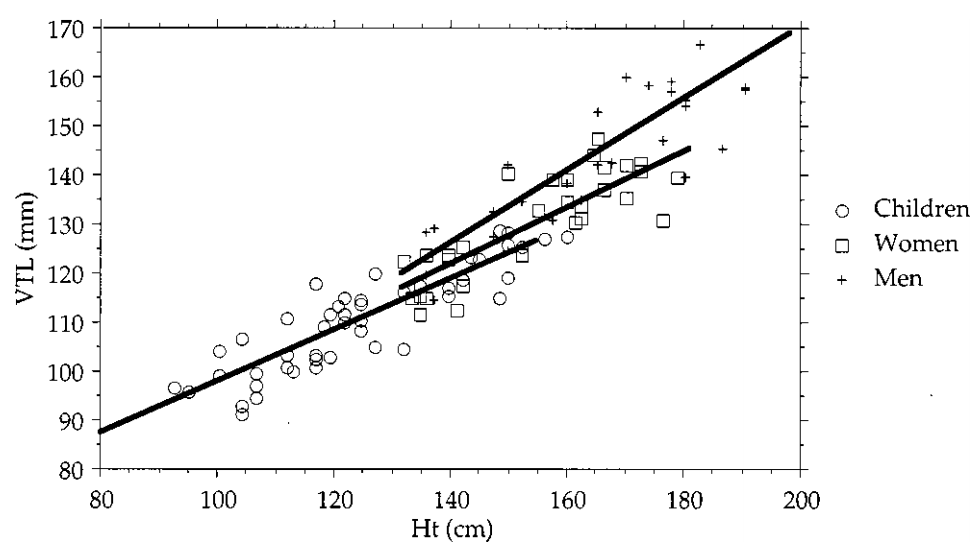
\includegraphics[width=.66\linewidth]{gfx/vocal-tract-size-sex.png}}
        \caption{Height (cm) versus vocal tract length (mm) \cite{Fitch1999}.}
        \label{fig:vocal-tract-morphology-sex}
\end{figure}

\begin{figure}[!h]
        \myfloatalign
        {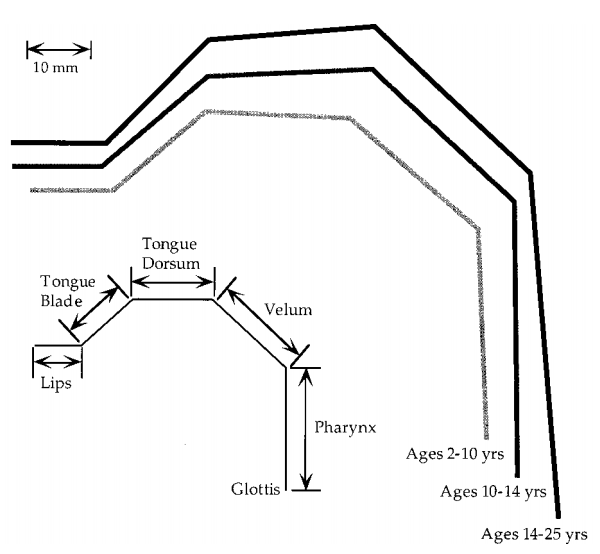
\includegraphics[width=.66\linewidth]{gfx/vocal-tract-size-gender.png}}
        \caption{Averaged vocal tract morphology \cite{Fitch1999}.}
        \label{fig:vocal-tract-morphology}
\end{figure}

As one can observe, men's vocal tract are longer than women's, followed and obviously children. These morphology differences 
affect the speech signal thorougly, specially in what concerns to the \ac{F0}. \ac{F0} can be defined as the 
lowest frequency in the signal counting from zero. \autoref{fig:f0-age-sex} compares the \ac{F0} values
between male and females considering aging.

\begin{figure}[!h]
        \myfloatalign
        {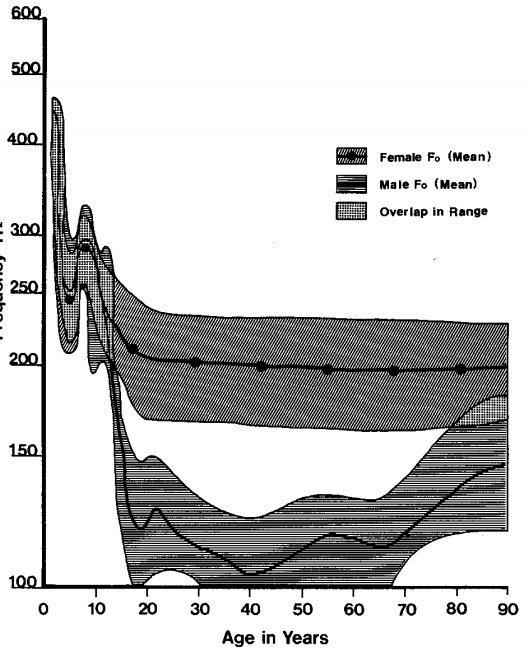
\includegraphics[width=.66\linewidth]{gfx/f0-age-sex.png}}
        \caption{F0 and pitch sigma versus age for males and females \cite{Brown1991}.}
        \label{fig:f0-age-sex}
\end{figure}

One can notice from \autoref{fig:f0-age-sex}, that no difference is found between male and female voice at a very young age. 
In fact, boys and girls have roughly the same \ac{F0} values. However, when they reach puberty, differences begin to appear. 
This period is commonly called the voice mutation or voice change, when the \ac{F0} for male voice has huge drop, while 
for female voice the drop is quite small. In terms of perception, this is period when the male voice lowers and geets deeper.

XXXXXXXXXXXXXXXXXXX EXTEND INTER-SPEAKER VARIABILITY
XXXXXXXXXXXXXXXXXXX DESCRIBE INTRA-SPEAKER VARIABILITY

But let's get back to \autoref{tab:comparison-human-mach}. It is interesting to notice that humans
performed better in all speech recognition tasks, but one: ``Clean speech based on trigram sentences''.
This one task consists of recognizing sentences which were randomly generated using the WSJ trigram language model. 
Therefore, humans had no advantage over machines in what concerns to syntactic or semantic knowledge. 
This result highlights one of the most important feature of human hearing, that is, we make a large use of syntactic, 
semantic and also pragmatic information in order to understand speech. While hearing do not take into account simply 
the acoustic signal, but the whole context. 

Language is a social tool, which aims at successfull interaction. When someone steps into a snack bar and orders 
an [\textipa{aIs"krim}], the vendor has no doubt that this sequence of phones refers to ``ice cream'' and not ``I scream'', 
albeit they are pronounced exactly the same. Although such sequence of phones might be ambiguous in the phonetic level,
it is not in higher linguistic levels, such as syntax (the verb ``order'' is usually followed by a noun), semantics 
(the object of order has to be something purchasable) and pragmatics (one does not buy his own shout!).


\section{HMM-based Speech Recognition} 
\ac{HMM} is the most widespread and successfull paradigm in \ac{ASR}. When \ac{HMM} were first applied
to speech recognition in the late $70$'s, they were completely revoluationary.
Up until recently \ac{DNN} seem to be next prominent paradigm in \ac{ASR}.
\ac{HMM} have been applied
to \ac{ASR} since the late $70$'s, and they have gathered the best results until recently.

A \ac{HMM} is a statistical Markov model in which the states are assumed to be hidden, i.e. they are
not directly visible, only the state's outputs are observable. Each state has a probability distribution 
over the possible output tokens, in such a way that output generated by the HMM states provides some information
about the hidden sequence of states which was traversed.

\section{Feature Extraction}

\subsection{Preambulus}
Feature extraction is an importart part of speech recognition systems. The feacture extraction 
phase is responsible for identifying or enhancing the components of the signal that are relevant 
for recognizing speech sounds, while discarding or diminishing the effect of unuseful information, 
such as background noise. With respect to speech parameterization, \ac{MFCC} are definitely the
standard. \ac{MFCC} have been widely used in \ac{ASR} systems for almost three decades \cite{Davis1980}, 
they are present on the many important speech recognition toolkits, such as \ac{HTK}, Sphinx, \ac{RASR} and Kaldi.
Before we go into further details about these features it is interesting to give a little background 
about speech recording and coding.

Speech is recorded by using a microphone -- nothing new so far!
Despite the many types of available microphones (condenser, capacitor, pyezoeletric, laser, etc.) its design
remains basically the same as the carbon microphone invented by David Hughes two centuries ago \cite{Robjohns2010}.
A microphone is simply an acoustic-to-electric sensor, which converts variations in air pressure (that is, sound)
into an electrical signal. Microphones have a very thin membrane, called diaphragm, which vibrates when struck by 
sound waves.  When the diaphragm vibrates, it puts to move a sensitive capsule attached to it, 
that converts its movement into electrical pulses. Most of the current microphones are dynamic, which means 
that their capsule consist of  .... (XXX VER WIIPEDIA)

After capturing speech through a microphone, one usually wants to store it for later access. In order
to store speech digitally on a computer, a coding scheme is mandatory. In the literature, many coding schemes have
been proposed, such as linear PCM, $\mu$-law, A-law PCM, APCM, DPCM, DM, and ADPCM \cite{Huang2001}. The details of 
each type of speech coder is beyond the scope of this dissertation, the reader can 
find an description of each scheme in \citeauthor{Huang2001} \citep{Huang2001} or \citeauthor{Furui2001} \citep{Furui2001}. 
Following we will give a brief discussion of linear PCM, which is the standard way of storing audios in digital format. 

\ac{PCM} is a type of analog-to-digital conversion, which constitutes the basis of the WAV digital audio format, together
with other lossless formats such as AIF and AU.
\footnote{Other types of popular audio files which use lossy data compression, such as MP3, WMA, OGG or AAC (a format common to 
DivX videos) do not use PCM. Instead}. 
PCM coding is based on two properties: (i) a sampling rate of the audio and a (ii) bit depth. The sampling rate determines the
number of audio samples that are taken per second from the signal, in turn the bit depth is the number of bits 
of information in each audio sample. Both values must be constant and should be defined prior to recording (actually coding) an audio. 
The sampling and the bit depth are closely related to the audio quality, that is, the higher the sampling and the depth
the better the fidelity of the digital audio to the analog speech signal. Picture XXX presents an example of a linear PCM 
representation, at different sampling rates and bit depths, of an audio containing the utterance ``Speech recognition''.

Linear PCM assumes that the discrete signal $x[n]$ is bounded, that is,
\begin{equation}
|x[n]| \leq X_{max} 
\end{equation}
and that the quantization step $\Delta$ is uniform for all consecutive levels of $x_i$
\begin{equation}
x_i - x_{i-1} = \Delta
\end{equation}

Assuming a binary code, the number of levels which can be represented by PCM is $N=2^B$, where $B$ is the bit depth, this constitutes
the audio resolution. According to \citep{Huang2001}, speech could be represented in an intelligible way by using 7 bits, however, in 
practice, applications use values no lower than 11 bits to guarantee communication efficiency. For instance, CDs makes use of 16-bit 
linear PCM, whereas DVD-Audio and Blu-Ray discs can support up to 24-bit.

Although linear PCM files are able to carry all the necessary auditory information -- after all we are able to listen to them and
recognize the speech, the music or the noise recorded in them; they are not useful for speech recognition purposes. This occurs 
because, from the phonological point of view, very little can be said based on the waveform itself \citep{Shrawankar2010}.
Consider, for instance, the two combinations of 100 Hz, 200 Hz and 300 Hz sine waves, shown in \autoref{fig:complex-waves-pure-tones}, 
which differ only with respect to the relative timing.

\begin{figure}[!h]
        \myfloatalign
        {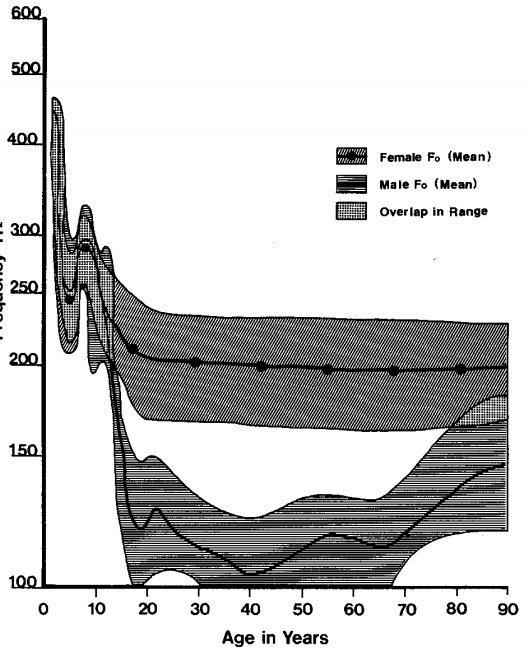
\includegraphics[width=.66\linewidth]{gfx/f0-age-sex.png}}
        \caption{Two complex waveforms generated by the same three pure tone 100 Hz, 200 Hz and 300 Hz sine waves, differing only 
        with respect to their relative timing \cite{Ladefoged1996}.}
        \label{fig:complex-waves-pure-tones}
\end{figure}
 
As one might notice, disregard of being composed by the same pure tones, the complex waves shown in 
\autoref{fig:complex-waves-pure-tones} are completely distinct from one another. This happens because the waveform is influenced
by phase shifts (also known as phase offsets). Therefore in-phase and out-of-phase waves (\autoref{fig:in-phase-waves} and
\autoref{fig:out-of-phase-waves}) are represented differently, and this adds too much variability to the waveform, in such way that
the signal waveform becomes unsuitable for human analysis and consequently for being used as a raw input in \ac{ASR} systems. 


\begin{figure}[!h]
        \myfloatalign
        {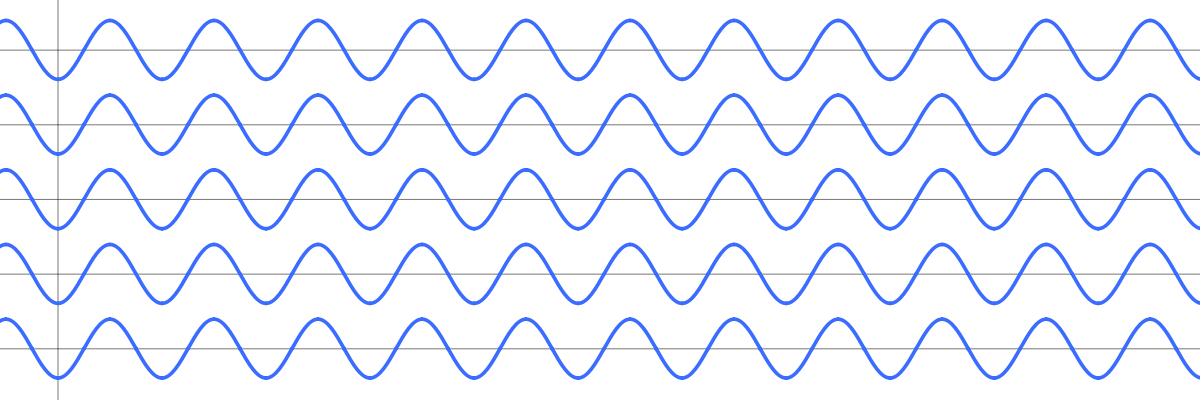
\includegraphics[width=.66\linewidth]{gfx/in-phase-waves.png}}
        \caption{Example of in-phase waves.}
        \label{fig:in-phase-waves}
\end{figure}

\begin{figure}[!h]
        \myfloatalign
        {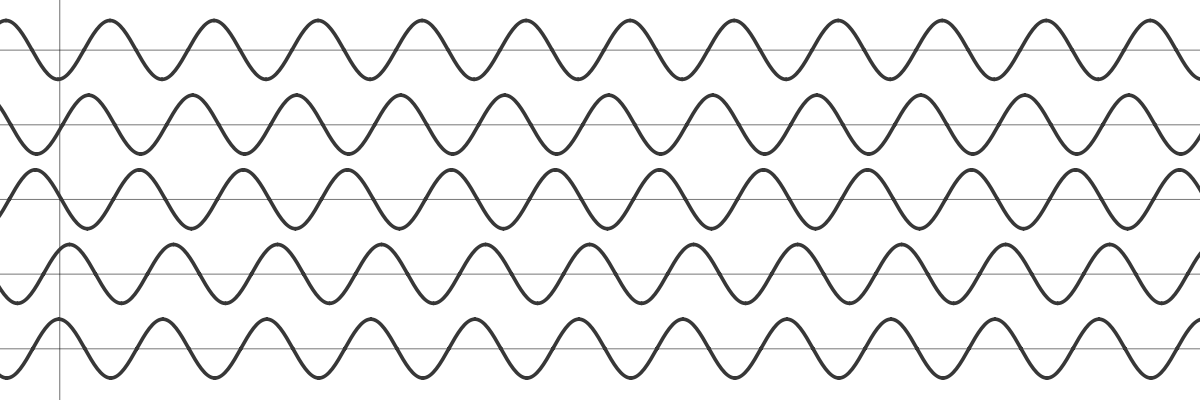
\includegraphics[width=.66\linewidth]{gfx/out-of-phase-waves.png}}
        \caption{Example of out-of-phase waves.}
        \label{fig:out-of-phase-waves}
\end{figure}

Another way of representing the audio information, which is more meaningful for human reading
or computer analysis is through short-term spectrum. Short-term spectra are obtained by applying
a Discrete Time Fourier transform to a windowed signal. At first, the signal is divided
into uniformly-spaced periods with a sliding window. For speech recognition, usually the window size is defined as 25 ms, 
with a frame shift of 10 ms, audio information is extracted every 10 ms with 15 ms of overlapping
among adjacent frames \cite{Huang2001}. \autoref{fig:audio-windowing} contains an example of a windowing process (in this case, 
with 50\% overlapping).

\begin{figure}[!h]
        \myfloatalign
        {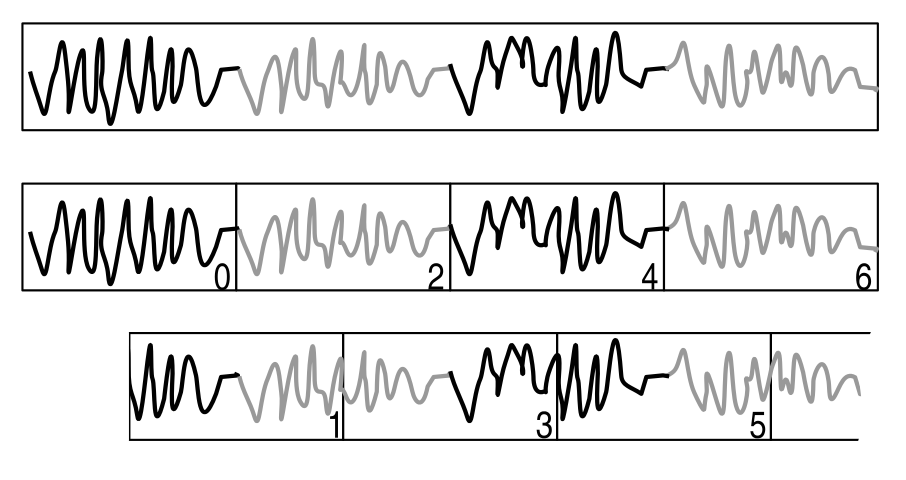
\includegraphics[width=.66\linewidth]{gfx/audio-windowing.png}}
        \caption{Illustration of an original audio recording (the upper waveform) divided into two
offset sequences of analysis windows (two lower waveforms) with 50\% overlapping frames \cite{McLoughlin2009}}
        \label{fig:audio-windowing}
\end{figure}

These windows values are based on two assuptions: (i) that within 25 ms the signal is stationary, i.e.
the phonatory system is not moving; (ii) that at least a period of each relevant speech frequency will 
be captured by this window
this windows, that is no relevant are 

After windowing the signal a Fourier transform is applied into each window so as to obtain
a series of frequency spectra, i.e. a series of representation of the signal in the frequency domain instead of the time domain. As can be noticed in \autoref{fig:audio-windowing}, since the frame shift is smaller than the window size, the windowing process extracts many redundant information. The intention for doing this will be made afterwards, when we give further details of the Fourier transform. Such transform is based on the Fourier theorem, which states that any periodic waveform can be approximated as closely as desired as the sum of a series of pure sine waves. In other words, the Fourier transform is able to analyse a short-term of the signal, containing a complex wave, and to output which are and what is the amplitude of the pure tones which form this complex wave.

Feature extraction must then be performed in stored audio files in order to extract relevant information from the waveform and discard redundant or unwanted signal characteristics. As already mentioned before, the two most traditional techniques for speech feature extraction, over the past decades, have been the \ac{MFCC} \cite{Davis1980} and the \ac{PLP} \cite{Hermansky1990}. Both parameterization methods are based on the short-term spectrum of speech. For speech recognition purposes, \ac{MFCC} features usually show better performance when compared to \ac{PLP}, for this reason in this thesis we are only going to present \ac{MFCC} features \cite{Muller2001, Mporas2007}.

\section{MFCC Features}

\ac{MFCC} is a type of speech parameterization is the result of a cosine transform of the logarithm of the short-term energy spectrum expressed over a mel scale \cite{Davis1980}. \ac{MFCC} features tries to reduce the feature dimensionality of a sound Fourier spectrum, by applying some concepts of Psychoacoustics and Psychophysics in order to the extract a vector with relevant values from the spectrum. The aim is to represent speech data in a compressed format, by eliminating information which are not pertinent to the phonetic analysis and to enhance the aspects of the signal which contribute to the detection of phonetic differences \cite{Davis1980}.

From Psychoacoustics, \ac{MFCC}s use the notion that humans do not perceive frequency through a linear scale, but through a scale which resembles to be linear-spaced in frequencies below 1000 Hz and logarithmic in frequecies above 1000 Hz\footnote{This is not entirely true. As shown by \citeauthor{Umesh1999}~\cite{Umesh1999}, in fact, there are no two distinguishable regions in terms of statistical significance. But the idea that we perceive low frequencies better than high ones still hold.}, the so-called mel scale (named after \emph{mel}ody). The scale is based on experiments with simple tones in which individuals are required to separat frequency values into four equal intervals or to adjust the frequency of a stimulus to be half as high as another reference tone \cite{Huang2001}. The reference point between mel scale and a linear frequency scale is 1000 mels, which correspond to a 1000 Hz tone, 40 dB above the absolute threshold of hearing. Since it was first introduced by \citeauthor{Stevens1937}~\cite{Stevens1937}, the scale has been revisited many times \cite{Umesh1999}, but a common formulation, according to \citeauthor{Huang2001}~\cite{Huang2001} is:
\begin{equation}
 M(f) = 1125*ln(1 + f / 700)
\end{equation}
where $f$ is the input frequency in Hz. The scale is plotted \autoref{fig:mel-scale}.
\begin{figure}[!ht]
        \myfloatalign
        {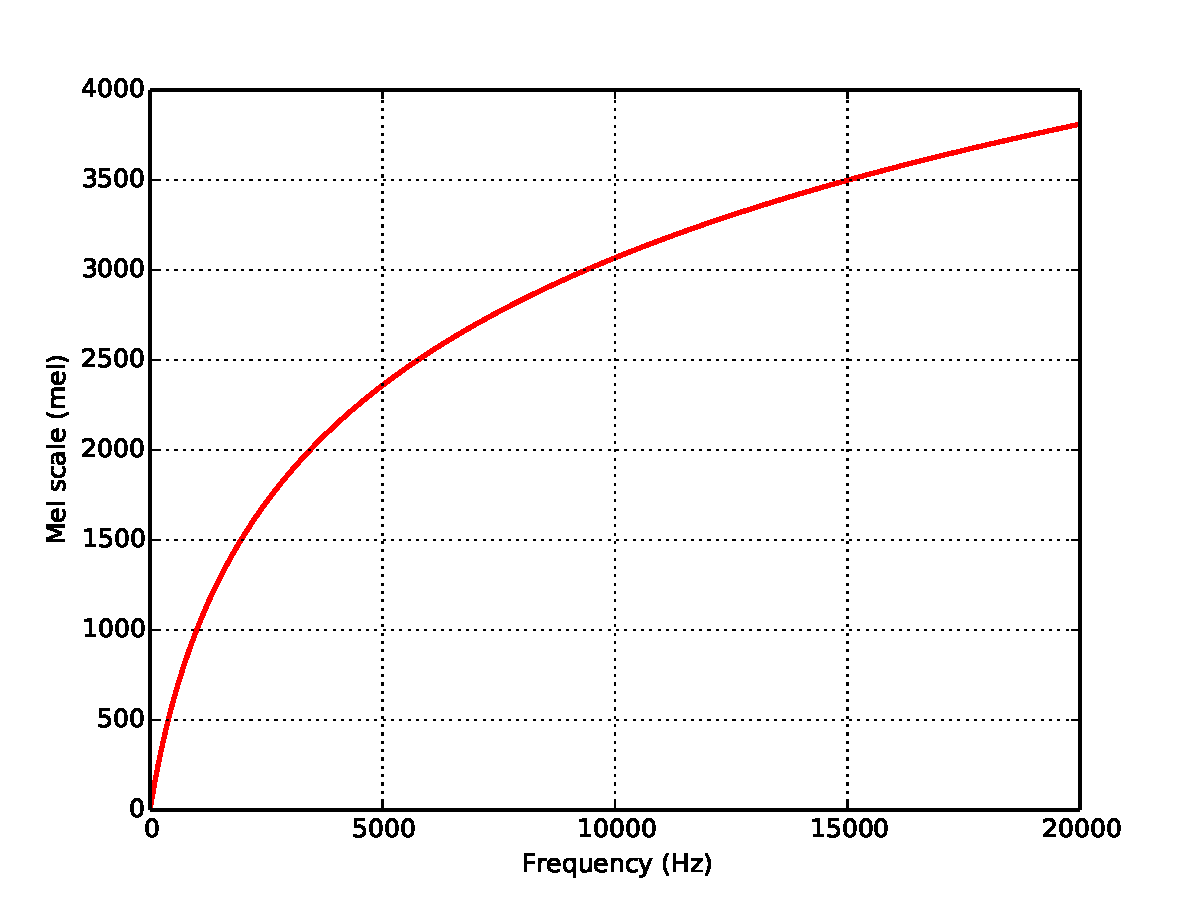
\includegraphics[width=1.\linewidth]{gfx/mel-scale.pdf}}
        \caption{Mel scale versus a linear frequency scale.}\label{fig:mel-scale}
\end{figure}

and also of the physics of speech, such as the fact that human like the these systems often have well defined overtones that are harmonic -- which is why the MFCCs use the FFT of the FFT)


\section{Dealing with Noisy Data}

One of the central problems in \ac{ASR} is how to deal with noisy audio data. It is long known that the performance of 
speech recognition systems greatly degrate when the environmental or the recording conditions are not controlled, 
thus allowing unwanted residual sounds to appear in the signal. In acoustics, any type of sound that is not the one
you are willing to analyze is considered noise. As a result from this, in speech recognition, the hiss of a fan, 
the buzz that a computer cooler makes, car horns on the street and so on are all regarded as noise. Even someone's voice
can be regarded as noise. Consider, for instance, that you are trying to recognize John's speech in an application, 
however Mary is close to him talking on the phone, to the extent that traces of her voice are added to the signal. In this
scenario, Mary's voice is actually noisy data, since it is undesirable for the given purpose. 


\section{Types of Speech Recognition Systems} 
Errem omnium ea per, pro \ac{UML} congue populo ornatus cu, ex qui
dicant nemore melius. No pri diam iriure euismod. Graecis eleifend
appellantur quo id. Id corpora inimicus nam, facer nonummy ne pro,
kasd repudiandae ei mei. Mea menandri mediocrem dissentiet cu, ex
nominati imperdiet nec, sea odio duis vocent ei. Tempor everti
appareat cu ius, ridens audiam an qui, aliquid admodum conceptam ne
qui. Vis ea melius nostrum, mel alienum euripidis eu.

\section{The Architecture of a Large Vocabulary Continuous Speech Recognition System} 
Non vices medical da. Se qui peano distinguer demonstrate, personas
internet in nos. Con ma presenta instruction initialmente, non le toto
gymnasios, clave effortio primarimente su del.\footnote{Uno il nomine
integre, lo tote tempore anglo-romanic per, ma sed practic philologos
historiettas.}


\ctparttext{This part addresses some fundamental concepts in Linguistics,
Acoustics, and Automatic Speech Recognition.}
\part{Related Work}\label{part:related-work}
%************************************************
\chapter{Computer Assisted Pronunciation Training}\label{ch:capt}
%************************************************

\section{PB}

1 Sistemas de Reconhecimento de Pron\'uncia

Um reconhecedor de pron\'uncia nada mais \'e do que um reconhecedor de fala
voltado a uma tarefa espec\'ifica, qual seja: compreender e analisar a
pron\'uncia de um aprendiz. Como j\'a discutido, um reconhecedor de fala \'e
um sistema computacional que recebe como entrada um sinal ac\'ustico de
fala e fornece como sa\'ida a transcri\c{c}\~ao textual da informa\c{c}\~ao contida na
fala (Rabiner \& Schafer, 2007).

Reconhecedores de pron\'uncia s\~ao ferramentas de interesse, especialmente,
na \'area de Computer-Assisted Language Learning (CALL), sub\'area da
Lingu\'istica Aplicada que se dedica ao estudo da utiliza\c{c}\~ao de
computadores para aprendizagem de l\'ingua (Beatty, 2002). Os sistemas de
CALL que auxiliam no aprendizado ou na pr\'atica da pron\'uncia de outras
l\'inguas s\~ao os chamados Computer-Assisted Pronunciation Training (CAPT).
Tais sistemas s\~ao \'utes, especialmente, por quatro motivos: (i) sua
difus\~ao: basta ter acesso a um computador para utiliz\'a-los; (ii) sua
capacidade de fornecer feedback individual - nas salas de aula
tradicionais, dado o tempo, nem sempre \'e poss\'ivel ao professor corrigir
verbatim a pron\'uncia de cada aluno; (iii) seu baixo custo - tais
tecnologias possuem baixo custo, se comparadas ao gasto com um curso de
pron\'uncia; (iv) sua possibilidade de propiciar autoestudo ass\'incrono - o
aluno pode treinar sua pron\'uncia onde e quando quiser, independentemente
de um lugar ou hor\'ario espec\'ifico (Witt, 1999).

Sistemas de CAPT, em geral, tentam agregar os  seguintes  componentes:

listas de pron\'uncia, material expositivo com informa\c{c}\~oes ac\'ustico-
articulat\'orias de cada som, tutoriais e exerc\'icios de transcri\c{c}\~ao,
atividade para pr\'atica e avalia\c{c}\~ao de pron\'uncia. Dois desses sistemas,
notadamente, Accent Master e Macmillan Education Sounds s\~ao analisados a
seguir.

O Accent Master \'e um software pago, que busca ensinar a pron\'uncia do AmE
a partir de atividades, exerc\'icios, jogos, v\'ideos expositivos e
anima\c{c}\~oes. A parte de exposi\c{c}\~ao e ensino de pron\'uncia do software \'e bem
completa e possui explica\c{c}\~oes detalhadas de como se produz cada fone do
AmE, al\'em de v\'ideos e anima\c{c}\~oes da posi\c{c}\~ao dos \'org\~aos do aparelho
fonador. O software possui vers\~oes espec\'ificas para a l\'ingua nativa do
aprendiz (atualmente, h\'a suporte para 21 l\'inguas, incluindo o PB). As
vers\~oes espec\'ificas compreendem uma descri\c{c}\~ao dos sons da l\'ingua nativa,
bem como instru\c{c}\~oes sobre quais aspectos de pron\'uncia devem ser focados.
Por\'em o Accent Master n\~ao possui um sistema de reconhecimento de fala
built-in. O treinamento de pron\'uncia d\'a-se da seguinte forma: primeiro,
o aprendiz ouve uma palavra em ingl\^es, tenta repeti-la, ent\~ao, o
software plota no monitor o oscilograma da palavra ouvida e de sua
tentativa, e cabe ao pr\'oprio aprendiz comparar se a realiza\c{c}\~ao foi
similar ou n\~ao. No entanto, deixar ao aprendiz a an\'alise do oscilograma
n\~ao constitui uma boa solu\c{c}\~ao, pois, mesmo considerando a enuncia\c{c}\~ao de
uma mesma palavra, a forma de um oscilograma \'e bastante vari\'avel e
depende de caracter\'isticas do aparelho fonador (Johnson \& Mullenix,
1997). Al\'em disso, trabalhos anteriores a respeito de Sistemas de CALL
j\'a questionaram o valor pedag\'ogico deste tipo de atividade (Neri et al.,
2008). A Figura 10 cont\'em algumas telas da interface do software Accent
Master.

                         [pic]  [pic]  [pic]

           Figura 10: Telas da interface do Accent Master.

O Macmillan Education Sounds: The Pronunciation App \'e um aplicativo de
ensino de pron\'uncia do ingl\^es para iPhone, iPad e Android. Trata-se de
um software com uso gratuito limitado e compras in-app, que foi
desenvolvido para treinamento da pron\'uncia tanto do AmE, quanto do BrE.
O app possui exerc\'icios de reading, writing e listening para treinar a
transcri\c{c}\~ao fon\'etica das palavras do ingl\^es. No entanto, n\~ao h\'a nenhum
tipo de introdu\c{c}\~ao à fonologia ou fon\'etica do ingl\^es, de modo que se
pressup\~oe que o usu\'ario j\'a tenha dom\'inio do Alfabeto Fon\'etico
Internacional (AFI) e das conven\c{c}\~oes de transcri\c{c}\~ao das palavras do
ingl\^es. Sendo assim, a utiliza\c{c}\~ao do software acaba por restringir-se a
aprendizes intermedi\'arios e avan\c{c}ados de ingl\^es que saibam utilizar o
Alfabeto Fon\'etico Internacional. O exerc\'icio de pron\'uncia \'e composto por
um dicion\'ario, que cont\'em o \'audio das palavras e que possibilita ao
aprendiz gravar sua pr\'opria fala e comparar com o \'audio existente no
dicion\'ario. O app n\~ao possui reconhecimento de fala e, por conseguinte,
n\~ao h\'a nenhum tipo de avalia\c{c}\~ao ou feedback da pron\'uncia do usu\'ario. A
Figura 11 cont\'em exemplos da interface do software gratuito.

                         [pic]  [pic]  [pic]

Figura 11: Telas da interface do software Macmillan Education - Sounds.

\section{English}

Many papers have confirmed the importance of feedback for adequate learning in second language
acquisition. Negative feedback has been investigated by (XXXXX) and positive feedback by (XXXXX).
For \ac{CAPT} systems the feedback to the user may be provided by many media: text, voice or video.

Definitely, the more complex and informative form of feedback is through video. \citeauthor{Badin2010} \citep{Badin2010}
developed a 3D talking head, that is able to display the articulation in an augmented mode,
by showing all major speech articulators, including those usually hidden such as the tongue or the velum. The talking
was called OroFacial Clone, and an example of its display can be found in \autoref{fig:badin-orofacial-clone}.

\begin{figure}[!htb]
        \myfloatalign
        {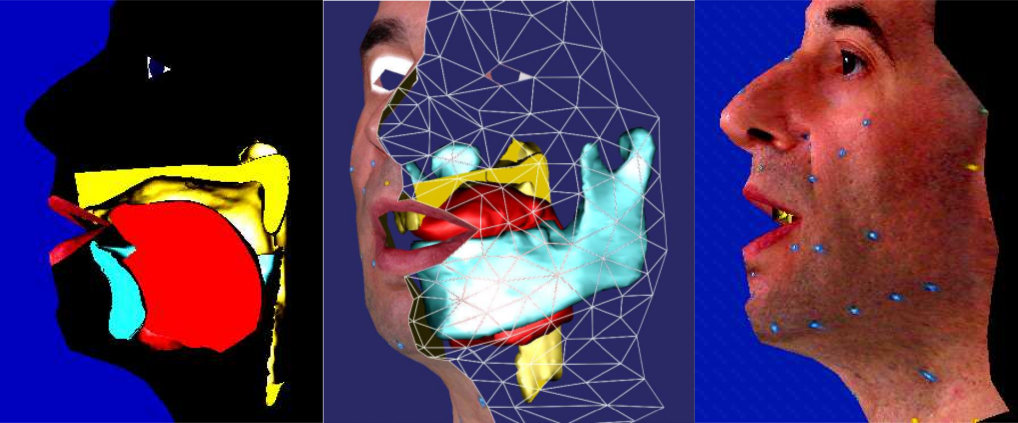
\includegraphics[width=.66\linewidth]{gfx/badin-orofacial-clone.png}}
        \caption{Example of the OroFacial Clone display, from \citeauthor{Badin2010} \citep{Badin2010}.}
        \label{fig:badin-orofacial-clone}
\end{figure}

The model is based on acustic-to-articulatory inversion and was built upon estimating speech articulators' 
movement from \ac{MRI}, \ac{CT} and video data. As one can imagine, building such a model is a very expensive task, which 
requires not only \ac{CG} and speech processing expertise, but also access to high-priced medical devices, such as 
\ac{MRI} scanners and tomographs. 

Part of this system was evaluated by \citeauthor{Wang2014} \citep{Wang2014} in a \ac{CAPT} context, by testing the
performance of Chinese learners of French. The aim of the test was to analyse the performance of the learners in the production 
and perception of the French vowels [\textipa{\o}] and [\textipa{\oe}], that do not exist in Chinese. The authors found that the 
students exposed to audiovisual stimuli produced vowels that were closer to the correct ones than the subjects who had access only 
to the auditory stimuli. After training, the difference between the F1 of [\textipa{\o}] and [\textipa{\oe}] was $62$ Hz for the audio
group and $178$ Hz for the audiovisual group. Additionaly, the audiovisual group performed better in 
an [\textipa{\o}] and [\textipa{\oe}] perception test, the number of correct responses rose from 61\% to 68\% for the audio only
group, and from 50\% to 86\% for the audiovisual one.




%*****************************************
%*****************************************
%*****************************************
%*****************************************
%*****************************************

%************************************************
\chapter{How to Adapt a Speech Recognition to Non-Native Data}\label{ch:how-to-adapt}
%************************************************
Lorem ipsum quod dolor sit amet.

\section{PB}


2 Adapta\c{c}\~ao a Dados de N\~ao-nativos

\'E ineg\'avel que as tecnologias de reconhecimento de fala, mesmo as do
estado da arte, apresentam problemas. Por tal raz\~ao, muitos
pesquisadores mostram- se c\'eticos quanto à efici\^encia do reconhecimento
de fala de n\~ao-nativos. Entretanto, as cr\'iticas que, geralmente, s\~ao
imputadas a sistemas de reconhecimento de fala de n\~ao-nativos, conforme
apontam Neri et al. (2003), s\~ao fruto da falta de familiaridade com o
design de reconhecedores de fala. De fato, caso se tente utilizar um
reconhecedor de fala, projetado para nativos, com n\~ao-nativos, o
desempenho ser\'a baixo, tendo em vista que o reconhecedor n\~ao est\'a
preparado para os padr\~oes ac\'ustico-articulat\'orios que o n\~ao-nativo
produzir\'a. Entretanto, h\'a diversos m\'etodos para se adaptar um sistema de
RAF a dados de n\~ao-nativos. Conforme apontam Strik e Cucchiarini (1999),
varia\c{c}\~oes de pron\'uncia de falantes n\~ao-nativos podem ser adicionadas a
qualquer n\'ivel do reconhecedor: no modelo ac\'ustico, no modelo de l\'ingua
ou no modelo de pron\'uncia. Tais modelos s\~ao apresentados nas tr\^es se\c{c}\~oes
seguintes.

3 Adapta\c{c}\~ao do Modelo Ac\'ustico (MA)

No que concerne ao modelo ac\'ustico do reconhecedor, tr\^es m\'etodos t\^em
sido, comumente, empregados para tratar dados de fala de n\~ao-nativos:
(i) adapta\c{c}\~ao ao falante; (ii) constru\c{c}\~ao de modelos bil\'ingues; e (iii)
utiliza\c{c}\~ao de modelos combinados, ou de interl\'ingua (Wang, et al.,
2003). Tais m\'etodos distinguem-se quanto à origem dos dados ac\'usticos
utilizados para treinar o modelo. Na adapta\c{c}\~ao ao falante, s\~ao
utilizados apenas dados de fala de falantes nativos da l\'ingua alvo. Na
constru\c{c}\~ao de modelos bil\'ingues, empregam-se no treinamento do modelo
ac\'ustico dados de fala de falantes nativos tanto da l\'ingua alvo, quanto
da l\'ingua base. Por fim, nos modelos combinados, ou de interl\'ingua, o
modelo ac\'ustico \'e treinado tendo em vista dados de falantes nativos da
l\'ingua alvo e, tamb\'em, de aprendizes. A Figura 12 resume as tr\^es
abordagens dispon\'iveis para adaptar o modelo ac\'ustico de um sistema de
RAF.

                                [pic]

Figura 12: M\'etodos para se adaptar o Modelo Ac\'ustico (MA) do
reconhecedor a dados de n\~ao-nativos.

A fim de melhor esclarecer a distin\c{c}\~ao que h\'a entre os tr\^es m\'etodos,
consideremos a cria\c{c}\~ao de um sistema de reconhecimento de pron\'uncia que
tenha por fim reconhecer o ingl\^es americano falado por falantes nativos
de PB. Na t\'ecnica de adapta\c{c}\~ao ao falante, para esse reconhecedor,
apenas dados de falantes nativos de ingl\^es seriam utilizados no
treinamento do modelo. Na abordagem bil\'ingue, o modelo ac\'ustico seria
composto de forma dual, possuindo dados de fala de ambas as l\'inguas:
tanto do ingl\^es americano, quanto do portugu\^es brasileiro. Na utiliza\c{c}\~ao
de modelos combinados ou de interl\'ingua, o modelo ac\'ustico seria
alimentado com dados nativos da l\'ingua alvo, no caso, americanos falando
ingl\^es, e tamb\'em com dados de aprendizes, isto \'e, brasileiros falando
ingl\^es.

Diversos m\'etodos e algoritmos podem ser empregados para realizar uma das
tr\^es abordagens de adapta\c{c}\~ao, a exemplo de: Maximum Likelihood Linear
Regression (MLLR) + Maximum A Posteriori (MAP) + Identifica\c{c}\~ao de fones
mais informativos (Oh et al., 2006), Phonetic Decision Tree (PDT) (Chen
\& Cheng, 2012), Polyphone Decision Tree Specialization (PDTS) (Wang et
al., 2003), Eigenvoices + MLLR (Tan \& Besacier, 2007), Phoneset comum +
Modelo multil\'ingue (Fischer et al., 2002). Nesta disserta\c{c}\~ao, propomos a
utiliza\c{c}\~ao de modelos combinados. De tal modo, ne

4 Adapta\c{c}\~ao no Modelo de Pron\'uncia (MP)

Em sistemas de RAF, os dicion\'arios de pron\'uncia constituem o m\'odulo que
cont\'em as palavras do l\'exico do reconhecedor, juntamente com sua forma
fon\'etica transcrita. Trata-se, em verdade, do componente do reconhecedor
que faz a ponte entre as unidades ac\'usticas subpalavras presentes no
modelo ac\'ustico e as poss\'iveis sequ\^encias de palavras especificadas no
modelo de l\'ingua. O Quadro 5 ilustra a estrutura do CMUdict{[}15{]}
(Weide, 1998), um dicion\'ario de pron\'uncia de refer\^encia para o ingl\^es
americano.

              Quadro 5: Exemplo de entradas no CMUdict.

                                [pic]

Como se observa, um dicion\'ario constitui uma lista de palavras, que
cont\'em formas ortogr\'aficas e fon\'eticas pareadas, al\'em de um
identificador. A fun\c{c}\~ao do identificador \'e possibilitar a distin\c{c}\~ao de
palavras hom\'ografas heter\'ofonas, isto \'e, palavras que possuem mesma
grafia mas pron\'uncia distinta, como gov{[}e{]}rno (nome) e gov{[}?{]}rno
(verbo); bem como a distin\c{c}\~ao das pron\'uncias variantes de uma palavra.

No que diz respeito ao RAF de n\~ao-nativos, a adapta\c{c}\~ao que se costuma
fazer ao dicion\'ario de pron\'uncia \'e a adi\c{c}\~ao das formas variantes de
pron\'uncia do n\~ao-nativo, de modo a construir os chamados dicion\'arios
multipron\'uncia. A constru\c{c}\~ao de tais dicion\'arios pode se dar por meio de
duas abordagens: (i) baseada em conhecimento ou (ii) baseada em dados
(Strik \& Cucchiarini, 1999). Ambas possuem seus pr\'os e contras.

Na abordagem baseada em conhecimento, variantes de pron\'uncia s\~ao
inseridas no dicion\'ario do reconhecedor por meio de regras geradas por
um especialista - um linguista. A l\'ingua constitui uma heterogeneidade
ordenada, isto \'e, a varia\c{c}\~ao n\~ao \'e um processo que ocorre
aleatoriamente, h\'a diversos fatores, sejam eles estruturais, sejam
sociais, que condicionam a varia\c{c}\~ao lingu\'istica (Weinreich, et al.,
2006). Portanto, cabe ao especialista explicitar a estrutura que subjaz
à varia\c{c}\~ao lingu\'istica, inferindo as regras fonol\'ogicas que melhor
descrevem as variantes. Tais regras, em geral, assumem o formato:

                            $A > B / C_D$,

em que A representa o elemento a ser modificado, B o elemento j\'a
modificado, e C\_D o contexto de aplica\c{c}\~ao da regra, sendo C o contexto
estrutural à esquerda e D o contexto à direita (Crystal, 2008). Regras
fonol\'ogicas, portanto, s\~ao capazes de descrever a varia\c{c}\~ao fon\'etica em
uma escala segmental (Wester, 2003). Considere-se, como exemplo, o caso
da ep\^entese de vogais altas anteriores n\~ao-arredondadas {[}i{]} em
s\'ilabas contendo oclusivas em coda, por brasileiros aprendizes de
ingl\^es. Por transfer\^encia de padr\~oes fonot\'aticos de L1 para L2,
brasileiros tendem a realizar ep\^entese em palavras que apresentam
oclusivas em posi\c{c}\~ao coda, que s\~ao proibidas, originalmente, na
fonologia do portugu\^es (Collischonn, 2003; Zimmer \& Alves, 2006). Sendo
assim, acabam por pronunciar ``book'' como boo{[}ki{]} em vez de
boo{[}k{]} e ``trip'' como tri{[}pi{]} em vez de tri{[}p{]}. Tal fato
pode ser capturado pela regra:

                      $COCLUS > COCLUS+[i] / _\$$,

em que COCLUS representa uma consoante oclusiva e ``\$'' a fronteira
sil\'abica. Na constru\c{c}\~ao de dicion\'arios multipron\'uncia baseados em
conhecimento, o especialista deve arrolar um conjunto suficiente de
regras, de forma a acomodar as diversas varia\c{c}\~oes de pron\'uncia que um
falante n\~ao-nativo apresenta.

Trata-se, portanto,  de  uma  tarefa  custosa,  quer  financeira  quer
temporalmente, uma vez que pressup\~oe um extenso levantamento e an\'alise
de dados lingu\'isticos ou uma consulta dicion\'arios transcritos j\'a
compilados. Al\'em disso, apesar de os dados obtidos com um especialista
serem fi\'aveis, frequentemente, o levantamento feito \'e incompleto, j\'a que
diversos fen\^omenos de varia\c{c}\~ao lingu\'istica ainda est\~ao para ser
estudados, n\~ao havendo literatura dispon\'ivel (Wester, 2003). Em outras
palavras, regras desenvolvidas por um especialista possuem alta precis\~ao
(precision), mas n\~ao necessariamente alta cobertura (recall). Ademais, a
abordagem baseada em conhecimento \'e dependente de l\'ingua ou, em certos
casos, de um dialeto; regras desenvolvidas para uma l\'ingua ou dialeto
n\~ao s\~ao necessariamente aplic\'aveis a outras l\'inguas ou dialetos.

A abordagem baseada em dados para a constru\c{c}\~ao de dicion\'arios
multipron\'uncia pode ser classificada como direta ou indireta (Kim, Oh,
\& Kiem, 2007). Na direta, padr\~oes de varia\c{c}\~ao existentes em um conjunto
de teste s\~ao analisados e utilizados, imediatamente, para gerar as
palavras variantes. J\'a na indireta, busca-se inferir regras que possam
ser aplicadas na gera\c{c}\~ao de uma ou mais variantes para uma palavra. A
abordagem direta, portanto, at\'em-se aos padr\~oes de varia\c{c}\~ao que ocorrem
no conjunto de teste, enquanto a indireta \'e capaz de prever padr\~oes que
n\~ao vieram a ocorrer.

Um dos problemas da utiliza\c{c}\~ao de dicion\'arios multipron\'uncia \'e o aumento
da incerteza do reconhecedor. Com a adi\c{c}\~ao de variantes ao dicion\'ario de
pron\'uncia, aumenta-se a cardinalidade do espa\c{c}o amostral de palavras que
o reconhecedor deve percorrer na busca e, por conseguinte, aumenta-se
sua confus\~ao. Em s\'intese, ao se adicionar muitas formas variantes ao
dicion\'ario de pron\'uncia, a confus\~ao inserida no modelo pode
contrabalancear os ganhos com uma forma fon\'etica mais precisa para as
palavras (Compernolle, 2001). Dicion\'arios multipron\'uncia, de tal forma,
devem procurar o ponto ideal entre o n\'umero de formas variantes
adicionadas e as formas can\^onicas. Kim et al. (2007) prop\~oem uma m\'etrica
para avaliar a confus\~ao de dicion\'arios multipron\'uncia, baseada no n\'umero
de variantes de pron\'uncia de cada palavra, nos fones que a comp\~oem e na
dist\^ancia de Levenshtein entres as palavras. Tal m\'etrica, chamada
Confusability Measure (CM), \'e definida formalmente como: seja {[}pic{]}
um dicion\'ario multipron\'uncia, composto por {[}pic{]} palavras, de
maneira que cada palavra {[}pic{]} possua {[}pic{]} variantes de
pron\'uncia, sendo {[}pic{]} a j-\'esima variante de pron\'uncia pertencente à
i- \'esima palavra, ent\~ao:

{[}pic{]}

onde {[}pic{]} \'e a dist\^ancia de Leveshtein entre {[}pic{]} e {[}pic{]},
e {[}pic{]} \'e o n\'umero de fones da variante de pron\'uncia {[}pic{]},
normalizado pelo n\'umero total de fones de todas as pron\'uncias de
{[}pic{]}, tal que:

                                [pic]

onde {[}pic{]} \'e definido como o n\'umero de fones da pron\'uncia {[}pic{]}.
O objetivo da CM \'e sistematizar a constru\c{c}\~ao de dicion\'arios
multipron\'uncia, estabelecendo um crit\'erio objetivo para a sele\c{c}\~ao das
palavras que devem compor o modelo. Palavras distintas, mas com contexto
fon\'etico similar s\~ao favorecidas pela m\'etrica, podendo-se selecion\'a-las
ao estabelecer um threshold.

Em muitas vezes, os ganhos em WER obtidos com a constru\c{c}\~ao de modelos de
pron\'uncia s\~ao baixos em raz\~ao da adi\c{c}\~ao ``cega'' de palavras ao
dicion\'ario. Jurafsky et al. (2001) demonstraram, por exemplo, que o
relaxamento de vogais no ingl\^es e a substitui\c{c}\~ao de segmentos s\~ao,
automaticamente, capturados por modelos ac\'usticos baseados em trifones,
n\~ao sendo necess\'ario, portanto, adicionar variantes ao dicion\'ario.
Outros tipos de varia\c{c}\~ao, como o apagamento de s\'ilabas, n\~ao s\~ao bem
modelados em trifones, de modo que \'e necess\'ario trat\'a-los no dicion\'ario
de pron\'uncia (Jurafsky, et al., 2001).

Diversas t\'ecnicas podem ser utilizadas para elaborar um dicion\'ario
multipron\'uncia, a exemplo de: Gaussian Densities Across Phonetic Models
(Sara\c{c}lar \& Khudanpur, 2000), Group Delay Based Segmentation (Brunet \&
Murthy, 2012), Phones Adaptation and Pronunciation Generalization (Ahmed
\& Ping, 2011), Automatic Generation of Accented Variants + MLLR
(Goronzy \& Eisele, 2003), Multi-span Linguistic Parse Tables (Mertens
et al., 2011), Decision Trees (Byrne et al., 1998), Pronunciation
Mixture Model (McGraw et al., 2008). A seguir, discutimos, em mais
detalhe, tr\^es desses trabalhos, notadamente: Sara\c{c}lar e Khudanpur
(2000), Matsunaga et al. (2003) e Kim et al. (2007).

Sara\c{c}lar \& Khudanpur (2000) prop\~oem uma t\'ecnica, a que chamam state
level pronunciation model (SLPM), que estima as pron\'uncias variantes de
uma palavra sem a inser\c{c}\~ao de variantes no dicion\'ario de pron\'uncia. Os
autores elaboraram um m\'etodo que permite que a representa\c{c}\~ao de um
fonema /f/, por exemplo, seja, no modelo ac\'ustico, diretamente mapeada
nos estados HMM de suas variantes {[}f1{]} e {[}f2{]}, criando assim um
modelo misto. Tal t\'ecnica \'e capaz de gerar variantes de pron\'uncia
automaticamente, mas pressup\~oe a utiliza\c{c}\~ao de dados anotados de forma
manual para bootstrap do modelo. O state level pronunciation model
(SLPM) foi testado com dados do ingl\^es americano, em uma por\c{c}\~ao do
corpus Switchboard (\textasciitilde{}4 horas, \textasciitilde{}100k
fones). O incremento em WER reportado foi de 1,7\% (valor absoluto), tal
valor corresponde à melhoria no reconhecedor dos valores de WER sem um
modelo de pron\'uncia (39,4\%) e com um modelo de pron\'uncia do tipo state
level pronunciation model (SLPM) (37,7\%).

  Matsunaga et al. (2003) utilizam dicion\'arios multipron\'uncia e  modelos

ac\'usticos combinados para tratar o ingl\^es falado por japoneses. Os
autores conduziram testes utilizando cinco m\'etodos: (i) l\'exico do ingl\^es
+ modelo ac\'ustico nativo; (ii) l\'exico com influ\^encia do japon\^es + modelo
ac\'ustico japon\^es; (iii) compara\c{c}\~ao de ambos os m\'etodos; (iv) l\'exico
japon\^es e ingl\^es + modelo ac\'ustico combinado; (v) l\'exico combinado +
modelo ac\'ustico combinado + penalidade para altern\^ancia de palavras
entrel\'inguas.

  Kim et al. (2007) propuseram um m\'etodo autom\'atico  de  cria\c{c}\~ao  de  um

dicion\'ario multipron\'uncia, atrav\'es de uma abordagem indireta baseada em
dados. De modo a criar um sistema de RAF n\~ao-nativo para coreanos
aprendizes de ingl\^es, os autores expandiram as formas can\^onicas do
reconhecedor e, ent\~ao, utilizaram uma medida de confus\~ao (CM), baseada
na dist\^ancia de Levenshtein, para atribuir um valor a cada variante de
pron\'uncia e excluir aquelas que apresentavam baixa confus\~ao. As
variantes foram geradas atrav\'es do seguinte procedimento: 1º) as
senten\c{c}as n\~ao- nativas foram reconhecidas atrav\'es de um reconhecedor de
fones; 2º) a sa\'ida do reconhecedor foi alinhada com a forma de pron\'uncia
can\^onica esperada atrav\'es de um algoritmo de programa\c{c}\~ao din\^amica
(algoritmo de Viterbi); 3º) padr\~oes de pron\'uncia variantes foram obtidos
a partir dos dados alinhados; 4º) regras de varia\c{c}\~ao de pron\'uncia s\~ao
derivadas dos padr\~oes de varia\c{c}\~ao, por meio de \'arvores de decis\~ao
(algoritmo C4.5); 5º) as regras de varia\c{c}\~ao s\~ao aplicadas ao restante do
l\'exico, de modo a gerar poss\'iveis candidatas a variantes de pron\'uncia. A
medida de confus\~ao (CM) \'e ent\~ao utilizada, de modo a excluir do modelo
de pron\'uncia as variantes que apresentam baixa confus\~ao. O corpus
utilizado no experimento foi uma por\c{c}\~ao do Wall Street Journal Database
(WSJ0) (\textasciitilde{}7.138 senten\c{c}as). A melhoria na taxa de WER
reportada foi de 1,34\% (valor absoluto), que corresponde a uma varia\c{c}\~ao
de 19,92\% a 18,58\%. O baseline utilizado foi uma por\c{c}\~ao de 340
palavras do CMU Pronouncing Dictionary.

5 Adapta\c{c}\~ao no Modelo de L\'ingua (ML)

{[}Esta se\c{c}\~ao do trabalho ser\'a realizada posteriormente, ap\'os elaborados
os modelos ac\'ustico e de pron\'uncia.{]}

\section{Adaptation Methods for the Acoustic Model}
Lorem ipsum quod dolor sit amet.

\section{Adaptation Methods for the Pronunciation Model}
Lorem ipsum quod dolor sit amet.

\section{Adaptation Methods for the Languaeg Model}
Lorem ipsum quod dolor sit amet.


%*****************************************
%*****************************************
%*****************************************
%*****************************************
%*****************************************



\ctparttext{Results and discussion.}
\part{The Design of Listener}\label{part:design-listener}

%*****************************************
\chapter{Methods}\label{ch:methods}
%*****************************************

\section{PB}

O reconhecedor de pron\'uncia ora proposto ser\'a implementado a partir do
motor de reconhecimento de fala Julius (Lee \& Kawahara, 2009). Nove
erros de pron\'uncia foram selecionados para serem tratados pelo Listener,
assumindo-se, como pron\'uncia padr\~ao, o General American (GA). O modelo
ac\'ustico ser\'a compilado a partir de tr\^es corpora. Um de falantes nativos
de ingl\^es: TIMIT Acoustic-Phonetic Continuous Speech Corpus{[}16{]}; e
outros dois de aprendizes: COBAI - Corpus Oral Brasileiro de Aprendizes
de Ingl\^es{[}17{]} e um corpus coletado especialmente para este trabalho,
composto por leitura de senten\c{c}as foneticamente balanceadas. O
dicion\'ario a ser empregado \'e o CMU Pronouncing Dictionary, ao qual ser\~ao
acrescentaremos as hip\'oteses de pron\'uncia dos aprendizes, por meio de
regras. O modelo de l\'ingua ser\'a gerado a partir da Simple English
Wikipedia em conjunto com um corpus de textos escritos por aprendizes de
ingl\^es, o COMAprend, um dos tr\^es corpus do projeto COMET da Faculdade de
Filosofia, Letras e Ci\^encias Humanas da Universidade de S\~ao Paulo. A
efici\^encia do reconhecedor ser\'a avaliada por meio de medidas de Word
Error Rate (WER), Character Error Rate (CER) e matrizes de confus\~ao,
aplicadas por meio de ten-fold cross validation sobre os dados dos
corpora coligidos. De modo a verificar a viabilidade do m\'etodo ora
proposto, um prot\'otipo do sistema foi elaborado e avaliado, detalhes s\~ao
apresentados na Se\c{c}\~ao .

4 MATERIAIS E M\'ETODOS

1 Levantamento dos Desvios de Pron\'uncia

Na classifica\c{c}\~ao dos erros de pron\'uncia, deu-se prioridade,
especialmente, aos erros de pron\'uncia que afetam a compreens\~ao e que s\~ao
apresentados em trabalhos que consideram, no ensino da pron\'uncia do
ingl\^es, a transfer\^encia de padr\~oes sonoros de L1 para L2.

A listagem dos erros de pron\'uncia a serem considerados pelo Listener foi
obtida a partir da consulta aos trabalhos de Zimmer (2004), Godoy
(2005), Zimmer et al. (2009) e Crist\'ofaro-Silva (2012). Tais trabalhos
analisam aspectos de transfer\^encia de L1 para L2 e estabelecem um m\'etodo
de ensino de pron\'uncia que leva em conta essa transfer\^encia, a fim de
otimizar o aprendizado pelo aluno. De tal maneira, centra-se o estudo no
ensino dos padr\~oes de pron\'uncia que devem ser enfatizados para o falante
do PB, a fim de melhor garantir a compreens\~ao de sua pron\'uncia e sua
efici\^encia comunicativa. No reconhecedor, optou-se por utilizar os nove
tipos de erros elencados em Zimmer et al. (2009), por se tratar da
investiga\c{c}\~ao mais abrangente sobre o assunto. Os desvios de pron\'uncia
selecionados est\~ao sintetizados no Quadro 5.

   Quadro 5: Desvios de pron\'uncias a ser analisados pelo Listener.

                                [pic]

2 Simplifica\c{c}\~ao sil\'abica

Um conjunto de 30 regras foi definido para gerar as variantes de
pron\'uncia envolvendo casos de simplifica\c{c}\~ao sil\'abica. As regras se
baseiam nos exemplos citados por Rauber e Baptista (2004), Rebello e
Baptista (2007), Zimmer (2009) e Silveira (2012). A discuss\~ao dos
contextos consta na Se\c{c}\~ao 2.1.1.4.1. O pseudoc\'odigo com a implementa\c{c}\~ao
das regras est\'a descrito na Figura 13.

Figura 13: Pseudoc\'odigo com regras para gera\c{c}\~ao das variantes de
pron\'uncia envolvendo simplifica\c{c}\~ao sil\'abica.

Como se observa, as regras de simplifica\c{c}\~ao sil\'abica buscam cobrir,
majoritariamente, quatro situa\c{c}\~oes: (i) oclusivas em posicao final de
palavra; (ii) palavras foneticamente terminadas em consoantes, mas com
\textless{}-e\textgreater{} final na forma escrita; (iii) clusters
consonantais em in\'icio de palavra do tipo /sC(C)/; (iv) palavras
iniciadas por /s ao/, com na forma ortogr\'afica.

3 O Motor de Reconhecimento de Fala Julius

Neste trabalho, propomos a utiliza\c{c}\~ao do motor de reconhecimento de fala
Julius (Lee \& Kawahara, 2009), como a base do reconhecedor de pron\'uncia
a ser desenvolvido. Julius \'e uma engine de alto desempenho e de c\'odigo
aberto para a constru\c{c}\~ao de sistemas de reconhecimento de fala. Ele
incorpora grande parte das t\'ecnicas do estado da arte em reconhecimento
de fala e executa Reconhecimento de Fala Cont\'inuo com Grande Vocabul\'ario
(LVCSR). Sua arquitetura est\'a sintetizada na Figura 14.

                                [pic]

Figura 14: Arquitetura do motor de reconhecimento de fala Julius (Lee \&
Kawahara, 2009).

Como se observa, ele suporta a entrada de dados de \'audio vindo de
microfone, de arquivos j\'a gravados, ou de streaming via internet. A
sa\'ida \'e composta ou por dados de textos, a exemplo de ditado, ou por uma
determinada a\c{c}\~ao solicitada ao Julius. No caso do reconhecedor de
pron\'uncia, a sa\'ida ser\'a constitu\'ida pela transcri\c{c}\~ao da fala e da
avalia\c{c}\~ao de sua pron\'uncia.

  Para  se  construir  um  reconhecedor  fala  atrav\'es  do  Julius,  s\~ao

necess\'arios: um modelo ac\'ustico, um dicion\'ario de pron\'uncia e um modelo
de l\'ingua. Mais detalhes sobre a elabora\c{c}\~ao desses modelos, de maneira a
possibilitar o desenvolvimento do reconhecedor de pron\'uncia, s\~ao
fornecidos a seguir.

4 Elabora\c{c}\~ao do Modelo Ac\'ustico

O modelo ac\'ustico proposto ser\'a elaborado atrav\'es de HMM e definido para
trifones. Julius prov\^e suporte a modelos ac\'usticos de HMM obtidos a
partir do HTK Hidden Markov Model Toolkit{[}18{]}, disponibilizado pelo
Speech Vision and Robotics Group, da Universidade de Cambridge. A
abordagem utilizada na elabora\c{c}\~ao do modelo ac\'ustico \'e a de interl\'ingua.
Portanto, ele ser\'a estimado a partir de dois tipos de corpora de fala:
um de falante nativos do ingl\^es: TIMIT Acoustic-Phonetic Continuous
Speech Corpus{[}19{]}; outros dois de falantes nativos do PB, aprendizes
de ingl\^es como L2: COBAI - Corpus Oral Brasileiro de Aprendizes de
Ingl\^es{[}20{]} - e um corpus coletado especificamente para o Listener,
composto por leitura de senten\c{c}as foneticamente balanceadas, isto \'e,
senten\c{c}as contendo fones de acordo com sua frequ\^encia de ocorr\^encia em
uma dada l\'ingua. A constru\c{c}\~ao de um modelo ac\'ustico interlingual busca
contornar a dificuldade de reconhecer a fala de n\~ao-nativos, atrav\'es da
inser\c{c}\~ao de informa\c{c}\~ao da pron\'uncia n\~ao-nativa no processo de
treinamento do modelo ac\'ustico, por meio de dados com a pron\'uncia dos
aprendizes (Wang, Schultz, \& Waibel, 2003).

5 Corpus de Nativos: TIMIT Acoustic-Phonetic Continuous Speech Corpus

Optou-se pela utiliza\c{c}\~ao do TIMIT (Garofolo, et al., 1993) como o corpus
de falantes nativos ingl\^es por se tratar de: um corpus bem modelado,
robusto, foneticamente rico, amplamente utilizado e testado na \'area de
reconhecimento de fala, em cerca de duas d\'ecadas de pesquisa, al\'em de
cobrir os dialetos majorit\'arios do ingl\^es americano (Lopes \& Perdig\~ao,
2011). O corpus TIMIT foi elaborado, conjuntamente, pelo Instituto de
Tecnologia de Massachusetts (MIT), SRI Internacional e Texas Instruments
Inc. (TI) com o prop\'osito fornecer dados para a realiza\c{c}\~ao de estudos de
fon\'etica ac\'ustica do ingl\^es, bem como para o desenvolvimento de sistemas
autom\'aticos de reconhecimento de fala. Ele cont\'em grava\c{c}\~oes de cerca de
630 falantes, dos oito principais dialetos do ingl\^es americano. As
grava\c{c}\~oes foram elaboradas a partir da leitura de dez senten\c{c}as criadas
artificialmente, de modo a capturar ambientes fon\'eticos relevantes. O
TIMIT foi verificado manualmente e est\'a transcrito ortogr\'afica e
foneticamente, adicionalmente, foi feito o alinhamento temporal entre o
arquivo de \'audio e as transcri\c{c}\~oes. Os arquivos est\~ao separados em
senten\c{c}a, amostrados a 16kHz com 16 bits por amostra. O TIMIT est\'a
dispon\'ivel para venda no Linguistic Data Consortium (LDC) e ser\'a
adquirido pelo N\'ucleo Interinstitucional de Lingu\'istica Computacional
(NILC).

6 Corpus de N\~ao-nativos: Corpus Oral Brasileiro de Aprendizes de Ingl\^es
(COBAI)

O COBAI (Mello, Avila, Neder-Neto, \& Orfano, 2012) constitui a primeira
iniciativa brasileira que busca compilar e distribuir, de forma aberta,
um corpus de fala anotado de aprendizes de ingl\^es, falantes nativos do
PB. O COBAI integra o Louvain International Database of Spoken English
Interlanguage (LINDSEI) e vem sendo organizado pelo Laborat\'orio de
Estudos Emp\'iricos e Experimentais da Linguagem (LEEL), da Faculdade de
Letras, da Universidade Federal de Minas Gerais (UFMG). O prop\'osito do
LINDSEI \'e a disponibiliza\c{c}\~ao de corpora de fala de aprendizes de ingl\^es,
com diferentes backgrounds de l\'ingua nativa. O COBAI segue as diretrizes
de transcri\c{c}\~ao do LINDSEI, que utiliza padr\~oes XML na anota\c{c}\~ao. A
transcri\c{c}\~ao \'e do tipo ortogr\'afica e agrega informa\c{c}\~oes de: troca de
turno, sobreposi\c{c}\~ao de fala, pausas, hesita\c{c}\~oes, formas reduzidas e
algumas indica\c{c}\~oes fon\'eticas e pros\'odicas. Atualmente, cerca de 60\% do
corpus est\'a anotado. O corpus consiste em 50 grava\c{c}\~oes de 15 minutos,
que incorporam uma narrativa, uma entrevista e uma descri\c{c}\~ao. Os
arquivos est\~ao separados e amostrados a 44kHz com 16 bits por amostra.
Todas as grava\c{c}\~oes foram feitas com falantes nativos do PB, aprendizes
de ingl\^es. O grau de conhecimento da l\'ingua inglesa dos participantes \'e
variado, havendo desde aprendizes com baixa profici\^encia at\'e indiv\'iduos
proficientes.

Uma contribui\c{c}\~ao colateral deste projeto ser\'a a finaliza\c{c}\~ao da
transcri\c{c}\~ao ortogr\'afica do COBAI e a anota\c{c}\~ao, no corpus, dos nove tipos
de erros que ser\~ao analisados pelo Listener. De modo a finalizar a
transcri\c{c}\~ao ortogr\'afica do COBAI, pretende-se utilizar um reconhecedor
de fala, no caso, o Dragon Naturally Speaking v.12 Premium, de modo a
obter uma transcri\c{c}\~ao ortogr\'afica inicial. A partir disso, realizaremos
a revis\~ao da transcri\c{c}\~ao, no intuito de corrigir os erros e adequar o
formato ao que \'e proposto pelo LINDSEI. Para a transcri\c{c}\~ao dos desvios
de pron\'uncia, prop\~oe- se o seguinte m\'etodo: ap\'os ter-se obtido a
transcri\c{c}\~ao ortogr\'afica de todo o corpus, ser\'a criado um script em
Python para percorrer cada palavra transcrita ortograficamente,
conferi-la no CMUdict e extrair a transcri\c{c}\~ao fon\'etica que l\'a est\'a
registrada. De tal forma, obteremos uma vers\~ao do COBAI transcrito com a
pron\'uncia can\^onica do General American (GA), que est\'a registrada no
CMUdict. A seguir, ser\'a realizada a revis\~ao do das transcri\c{c}\~oes
fon\'eticas, corrigindo-as quando os aprendizes cometerem algum dos nove
tipos de erros que o Listener avaliar\'a.

7 Corpus de N\~ao-nativos: Corpus de Leitura de Senten\c{c}as Foneticamente
Balanceadas por Aprendizes

A inten\c{c}\~ao inicial do projeto era utilizar apenas o COBAI como corpus
fala de n\~ao-nativos. Por\'em, ap\'os ter-se desenvolvido o prot\'otipo do
reconhecedor, conforme ser\'a descrito na Se\c{c}\~ao , foi poss\'ivel observar
que muitos dados do COBAI ter\~ao de ser desconsiderados e, de tal forma,
somente o COBAI n\~ao ser\'a suficiente para fornecer o n\'umero de horas
necess\'ario para a estima\c{c}\~ao de um bom modelo ac\'ustico. Por isso,
decidiu-se criar um corpus espec\'ifico para o desenvolvimento deste
trabalho.

O prop\'osito \'e compilar um corpus de aprendizes, em situa\c{c}\~ao de leitura
de frases pr\'e-definidas, foneticamente balanceadas, o qual seja gravado
em um ambiente com isolamento ac\'ustico. Os objetivos, com isso, s\~ao
tr\^es: i) assegurar a boa qualidade do \'audio, mantendo baixa a rela\c{c}\~ao
sinal-ru\'ido; ii) garantir que todas as combina\c{c}\~oes de trifones estejam
presentes na base de dados do modelo ac\'ustico, uma vez que as senten\c{c}as
ser\~ao foneticamente balanceadas; e iii) facilitar a tarefa de
transcri\c{c}\~ao, j\'a que a dura\c{c}\~ao da pesquisa de mestrado \'e curta. Prop\~oe-se
seguir as diretrizes de compila\c{c}\~ao e anota\c{c}\~ao de corpora, tal como
descrito por Hovy e Lavid (2010).

Pretende-se que os detalhes do m\'etodo de compila\c{c}\~ao e anota\c{c}\~ao do corpus
sejam definidos em visita t\'ecnica a ser realizada na Universidade de
Coimbra, sob supervis\~ao da Profa. Sara Candeias, no per\'iodo de 28 de
janeiro a 28 de fevereiro de 2014. O plano de tarefas proposto para a
visita inclui:

a defini\c{c}\~ao do tamanho do corpus a ser compilado;

a defini\c{c}\~ao do n\'ivel de detalhe da transcri\c{c}\~ao fon\'etica (qual o
invent\'ario de fones e xenofones utilizar);

a defini\c{c}\~ao do tipo de hesita\c{c}\~ao ou disflu\^encia a ser anotada;

a discuss\~ao de uma m\'etrica de riqueza fon\'etica (?), proposta para a
extra\c{c}\~ao de senten\c{c}as foneticamente balanceadas;

o teste e a avalia\c{c}\~ao da m\'etrica, a partir de um corpus de textos de
aprendizes de ingl\^es, o COMAprend.

No que diz respeito às senten\c{c}as foneticamente balanceadas, h\'a, para o
ingl\^es, diversas listas dispon\'iveis, como as Harvard Sentences (IEEE,
1969), os TIMIT Sentence Prompts (Garofolo, et al., 1993), as
MOCHA-TIMIT Sentences (Wrench, 1999), al\'em de diversas listas fornecidas
pela Carnegie Mellon University para o motor de reconhecimento Sphinx
(Lee, Hon, \& Reddy, 1990). No entanto, dado que essas listas foram
elaboradas para falantes nativos de ingl\^es, h\'a diversas palavras de
baixa frequ\^encia, bem como senten\c{c}as cuja estrutura sint\'atica \'e pouco
usual. Em um contexto de aprendizes, isso \'e problem\'atico, pois pode
ocasionar disflu\^encias na fala do aprendiz, causando problemas na
utiliza\c{c}\~ao dos dados, al\'em de padr\~oes de pron\'uncia altamente
irregulares, quando o aprendiz desconhecer a palavra que est\'a lendo.

Para contornar o problema, objetivamos criar um conjunto de senten\c{c}as
foneticamente balanceadas, a partir de um corpus de texto de brasileiros
aprendizes de ingl\^es, como o COMAprend (Tagnin \& Fromm, 2009). O
COMAprend possui textos em formato ortogr\'afico. A fim de se obter a
transcri\c{c}\~ao fon\'etica dos textos, ser\'a elaborado um script semelhante ao
descrito, anteriormente, na Se\c{c}\~ao 3.1.3.2.

8 Elabora\c{c}\~ao do Dicion\'ario de Pron\'uncia

O dicion\'ario de pron\'uncia ser\'a formado com base no CMU Pronouncing
Dictionary, o qual ser\'a acrescido de transcri\c{c}\~oes das poss\'iveis
pron\'uncias desviantes dos aprendizes, por meio de regras
transformacionais. Dicion\'arios contendo tais caracter\'isticas s\~ao tamb\'em
chamados na literatura como dicion\'arios multipron\'uncia (Strik \&
Cucchiarini, 1999).

9 CMU Pronouncing Dictionary

A base do dicion\'ario provir\'a do CMU Pronouncing Dictionary (tamb\'em
conhecido por CMUdict), disponibilizado no motor de reconhecimento de
fala Sphinx, pela Universidade Carnegie Mellon. O CMUdict constitui um
dicion\'ario de pron\'uncia machine readable de refer\^encia na \'area de
reconhecimento de fala. Atualmente, nele est\~ao registradas 131.411
entradas, transcritas foneticamente em formato ARPAbet (Zue \& Seneff,
1988). O Quadro 6 ilustra a entrada de algumas palavras no dicion\'ario.

Quadro 6: Exemplo de entradas no dicion\'ario de pron\'uncia do CMU
Pronouncing Dictionary.

                                [pic]

Como se observa, o dicion\'ario possui tr\^es campos: (i) um interno, para
identifica\c{c}\~ao da palavra, (ii) um com a palavra em sua forma
ortogr\'afica, convencionalizada em letras mai\'usculas, (iii) e um \'ultimo
campo com a transcri\c{c}\~ao fon\'etica da palavra, em formato ARPAbet.

10 Adi\c{c}\~ao das Formas Variantes de Pron\'uncia do Aprendiz

Ser\~ao utilizadas regras transformacionais para acrescentar ao dicion\'ario
as poss\'iveis hip\'oteses de pron\'uncia do aprendiz. A utiliza\c{c}\~ao de regras
transformacionais \'e de f\'acil implementa\c{c}\~ao computacional, correspondendo
a simples estruturas de sele\c{c}\~ao, ou constru\c{c}\~oes condicionais. Contexto
para aplica\c{c}\~ao de regras, como os elencados no Quadro 7, ser\~ao
levantadas, de acordo com a literatura lingu\'istica de ASL, e utilizados
para as variantes de pron\'uncias do aprendizes, a partir das palavras do
CMUdict. Casos marginais, de contexto muito restrito ou que n\~ao se
adaptem às regras criadas, ser\~ao adicionados, manualmente, em formato de
dicion\'ario de exce\c{c}\~oes.

Quadro 7: Contextos para aplica\c{c}\~ao de regras de simplifica\c{c}\~ao sil\'abica.

                                [pic]

11 Elabora\c{c}\~ao do Modelo de L\'ingua

Um modelo de l\'ingua ser\'a fornecido ao Listener, de modo a possibilitar
seu uso em um contexto de ditado. H\'a diversos modelos de l\'ingua para o
ingl\^es (como o Gigaword{[}21{]}, CSR LM-1{[}22{]}, HUB4{[}23{]}). Por\'em
a grande maioria desses modelos foi gerada a partir de corpora de
artigos de jornal e \'e sabido que textos jornal\'isticos de jornais
tradicionais, para p\'ublicos A, B e C tendem a possuir estrutura
sint\'atica e vocabul\'ario complexos, dado que as primeiras ora\c{c}\~oes de uma
not\'icia tendem a compactar muita informa\c{c}\~ao e podem trazer jarg\~ao n\~ao
dominado por aprendizes (Canning, 2002). Como a inten\c{c}\~ao \'e lidar com a
fala de aprendizes, propomos a cria\c{c}\~ao de um modelo de l\'ingua que seja
mais simplificado e condizente com a sintaxe dos aprendizes. Ser\'a
elaborado um modelo de l\'ingua estat\'istico, que considera trigramas na
an\'alise e se baseia em HMMs.

12 Simple English Wikipedia

Como corpus para cria\c{c}\~ao do modelo de l\'ingua, utilizaremos a Simple
English Wikipedia, cuja proposta \'e desenvolver uma Wikipedia em ingl\^es
de n\'ivel b\'asico, com vocabul\'ario e constru\c{c}\~oes sint\'aticas mais simples,
de modo a prover acesso a crian\c{c}as, estudantes, adultos com baixo n\'ivel
de letramento e aprendizes de ingl\^es como L2. A vers\~ao dispon\'ivel da
Simple English Wikipedia, referente ao dia 16 de janeiro de 2014, possui
108.665{[}24{]}. Todos os arquivos est\~ao codificados em XML. A
ferramenta SRILM (The SRI Language Modeling Toolkit){[}25{]} ser\'a
utilizada para auxiliar na cria\c{c}\~ao do modelo de l\'ingua.

13 Elabora\c{c}\~ao da Interface Web

A interface web desenvolvida para o Listener emprega conceitos de
gamifica\c{c}\~ao, com o prop\'osito de estimular a participa\c{c}\~ao dos usu\'arios e
de tornar o processo de aprendizagem mais apraz\'ivel.

14 Gamifica\c{c}\~ao

Segundo o historiador Huizinga (1938), um jogo constitui:

``uma atividade ou ocupa\c{c}\~ao volunt\'aria, exercida dentro de certos e
determinados limites de tempo e de espa\c{c}o, segundo regras livremente
consentidas, mas absolutamente obrigat\'orias, dotado de um fim em si
mesmo, acompanhado de um sentimento de tens\~ao e de alegria e de uma
consci\^encia de ser diferente da 'vida cotidiana'' (Huiziga 1938).

Jogos t\^em, desde sempre, fascinado as pessoas. Milh\~oes de pessoas vibram
e se emocionam ao assistir a uma partida de futebol de seu time
preferido. Mestres do xadrez, como Garry Kasparov, chegam a dedicar
cerca de seis horas di\'arias para dominar o jogo (ICC, 1998). Massive
Multiplayer Online Role Playing Games mobilizam milh\~oes de pessoas
online a um mesmo tempo. H\'a, tamb\'em, casos tr\'agicos, como o do taiwan\^es
que teve problemas vasculares e faleceu, logo ap\'os jogar Diablo 3 em uma
lan-house por 40 horas ininterruptas (Daily Mail, 2012).

De acordo com Lazzaro (2004), as pessoas jogam, basicamente, por um
dentre os quatro motivos a seguir: (i) pelo divertimento que o jogo
proporciona, (ii) pela competitividade que ele incita, (iii) pelas
sensa\c{c}\~oes diversas que ele pode gerar - surpresa, alegria, temor, etc.;
e (iv) pelo pretexto para socializar com os amigos. Jogos bem desenhados
tendem sempre a explorar esses pontos, a fim de fidelizar jogadores.

Deburr (2013) define a gamifica\c{c}\~ao a aplica\c{c}\~ao de estrat\'egias e t\'ecnicas
usadas no design de jogos em outros contextos, que n\~ao jogos. Zicherman
e Cunningham (2013) trazem uma defini\c{c}\~ao an\'aloga, para os autores a
gamifica\c{c}\~ao \'e ``o processo de utilizar a mec\^anica dos jogos no intuito
de motivar usu\'arios a resolver problemas'', sendo que a mec\^anica
comporta sete aspectos: (i) sistema de pontos, (ii) n\'iveis, (iii)
rankings, (iv) atribui\c{c}\~ao de t\'itulos, (v) desafios/miss\~oes, (vi) busca
de jogadores e (vii) um loop de est\'imulo social constante. Explicar cada
um desses aspectos

A gamifica\c{c}\~ao tem sido aplicada com sucesso a uma gama de contextos. H\'a,
por exemplo, comunidades de perguntas e respostas, como Stackoverflow e
Yahoo! Respostas, que a empregam a fim de motivar seus usu\'arios a
participarem da comunidade e a cooperarem entre si. Os usu\'arios que
fornecem as melhores respostas recebem pontos no site, sobem n\'iveis,
melhoram nos rankings, tornando-se cada vez mais influentes na
comunidade. Aplicativos para celulares que incitam a pr\'atica de corrida,
como o Runstatic e o Nike+, tamb\'em t\^em utilizado a gamifica\c{c}\~ao com
\^exito. Tais aplicativos extraem dados do percurso do usu\'ario via GPS e
lhes fornece estat\'isticas de sua corrida, de maneira que os usu\'arios
podem monitorar suas corridas para vencer metas, bater recordes pessoais
e, tamb\'em, competir com os amigos. \'E poss\'ivel tamb\'em desafiar outros
usu\'arios, para ver quem corre mais r\'apido, quem faz um mesmo percurso
maior em menor tempo, etc.

No \^ambito da educa\c{c}\~ao, a gamifica\c{c}\~ao tem sido explorada no chamado
edutainment - palavra am\'algama formada a partir de education e
entertainment (XXX:XX). Segundo Zicherman e Cunningham (2013), a
ind\'ustria tem falhado em utilizar a gamifica\c{c}\~ao para aplica\c{c}\~oes
educacionais. Muitas vezes, o aspecto instrucional \'e ressaltado de
maneira exagerada, de modo que os jogos se tornam chatos e as pessoas se
sentem desmotivadas para jog\'a- los. Para os autores, o jogo educacional
que melhor explorou os aspectos da gamifica\c{c}\~ao foi ``Where in the World
Is Carmen Sandiego?'', cujo prop\'osito \'e ensinar Geografia, mais
especificamente, o nome e a localiza\c{c}\~ao dos pa\'ises e de suas capitais.
Em ``Where in the World Is Carmen Sandiego?'', o jogador encarna um
detetive que deve juntar pistas para encontrar a criminosa Carmen
Sandiego. Ao longo da jornada, o jogador visita v\'arios pa\'ises e encontra
pessoas que lhe d\~ao pistas sobre onde Carmen Sandiego pode estar
escondida. As pistas cont\^em informa\c{c}\~oes gerais sobre os pa\'ises, como
``Uma pessoa suspeita veio aqui e disse que iria viajar à terra dos
Vikings'' ou ``Eu a vi embarcando em um avi\~ao cuja bandeira era vermelha
e azul''. A Figura 15 apresenta uma tela do jogo.

  Figura 15: Captura de tela do jogo "Where in the World Is Carmen
                             Sandiego?".

``Where in the World Is Carmen Sandiego?'' foi lan\c{c}ado em 1985 e, desde
ent\~ao, diversas empresas de edutainment t\^em tentado repetir o sucesso do
jogo, mas sem muito \^exito. Merece destaque o lan\c{c}amento, em 2012, da
plataforma para ensino de idiomas Duolingo (XXX:XX), que emprega
gamifica\c{c}\~ao e, s\'o no Brasil, j\'a consta com cerca 6,8 milh\~oes de
alunos{[}26{]}. Como se trata de uma aplica\c{c}\~ao de ensino de l\'inguas que
possui tamb\'em um m\'odulo de ensino de pron\'uncia, o Duolingo ser\'a tratado
em mais detalhes na Se\c{c}\~ao XXX.

The leaderboard of today has seensome radical redesign since the heyday
of pinball machines and quarter arcades. In the era of Facebook and the
social graph, leaderboards are mostly tools for creating social
incentive

In many instances, such as losing weight or even writing a book, it's
difficult for a player to understand where he is at the outset or during
early interactions. Moreover, the length and complexity of the overall
journey is such that sometimes players can be paralyzed by the seeming
lack of progress. Especially in health, education, and other ``epic
journey'' contexts, feedback forms the most important overarching game
mechanic, intricately tied to score and progress.

LER Jon Radoff's Game On

LER Jesse Schell's The Art of Game Design: A Book of Lenses

Segundo Zicherman e Cunningham (2013), como modelo de neg\'ocios, a
gamifica\c{c}\~ao transforma a rela\c{c}\~ao empresa-usu\'ario em uma rela\c{c}\~ao
simbi\'otica, cujo benef\'icio para o usu\'ario \'e o prazer obtido com o jogo e
para a empresa \'e a fideliza\c{c}\~ao do usu\'ario com o produto oferecido.

O corpus de erros induzidos

Para este prot\'otipo, reduziu-se a cria\c{c}\~ao do corpus de leitura de
senten\c{c}as foneticamente balanceadas a uma tarefa mais simples. Um
informante do sexo masculino foi gravado, lendo palavras em isolamento
e, propositalmente, enunciando-as com erros de transfer\^encia de L1 para
L2, a fim de simular variantes de pron\'uncia que ocorrer\~ao no corpus. As
palavras foram selecionadas a partir da lista das 5.000 palavras mais
frequentes da l\'ingua inglesa, segundo o Corpus of Contemporary American
English (COCA){[}29{]}. Cerca de 2h20min de fala foram compiladas. A
grava\c{c}\~ao ocorreu em uma sala fechada, com baixo ru\'ido externo, n\~ao
isolada acusticamente.

O COCA \'e o maior corpus de ingl\^es dispon\'ivel atualmente, tendo sido
compilado a partir de cerca de 160.000 textos escritos e transcritos, de
v\'arios g\^eneros, os quais totalizam 450 milh\~oes de tokens. O projeto \'e
coordenado por Mark Davies, professor de Lingu\'istica de Corpus da
Brigham Young University (BYU). O corpus \'e gratuito, mas as listas de
frequ\^encia s\~ao pagas, a exce\c{c}\~ao da menor delas, contendo as 5.000
palavras mais frequentes do ingl\^es, a qual foi utilizada no prot\'otipo.

Um script em Python foi elaborado para aplicar à lista as regras de
simplifica\c{c}\~ao sil\'abica elencadas na Figura 18. Quando havia contexto
para aplica\c{c}\~ao de qualquer uma das regras, a palavra era selecionada e
adicionada a um banco de palavras. Figura 18 sintetiza o funcionamento
do script. Das 5.000 palavras mais frequentes no COCA, 1.855
apresentaram contexto em que \'e poss\'ivel haver simplifica\c{c}\~ao sil\'abica,
tais palavras, portanto, foram selecionadas para leitura.

                                [pic]

Figura 18. Fluxograma de funcionamento do script seletor de palavras.

Um microfone condensador de diafragma pequeno (1/2``), com padr\~ao polar
cardi\'oide, do tipo Superlux S241/U3 foi utilizado nas grava\c{c}\~oes. O
microfone foi ligado a uma mesa de som anal\'ogica Yamaha MG102, atrav\'es
de cabos balanceados XLR, e alimentado por corrente fantasma (48V). A
capta\c{c}\~ao do \'audio se deu por um laptop LG A51, via cabos RCA. O software
Audacity (Mazzoni \& Dannenberg, 2000) foi usado na capta\c{c}\~ao, tendo-se
ativado o filtro supressor de ru\'ido. O ambiente de grava\c{c}\~ao consistiu de
uma sala fechada, sem isolamento ac\'ustico, em situa\c{c}\~ao de baixo ru\'ido
externo.

Os dados foram segmentados atrav\'es do Adintool, de forma similar ao
m\'etodo descrito na Se\c{c}\~ao 3.4.1.1. O Appendix II re\'une os par\^ametros
utilizados na segmenta\c{c}\~ao. Os arquivos foram alinhados com sua
transcri\c{c}\~ao ortogr\'afica, manualmente. A seguir, procedeu-se à
transcri\c{c}\~ao fon\'etica das palavras, de forma tamb\'em manual. Detalhes
sobre a transcri\c{c}\~ao constam, a seguir, na Se\c{c}\~ao 3.4.2.

O software Praat (Boersma \& Weenink, 2014) foi utilizado na
transcri\c{c}\~ao, para visualizar o espectrograma e, tamb\'em, tocar os
arquivos de \'audio. O LibreOffice Calc (The Document Foundation, 2014)
foi empregado para facilitar a organiza\c{c}\~ao das transcri\c{c}\~oes. Aten\c{c}\~ao
especial foi dedicada à an\'alise da ocorr\^encia ou n\~ao do fen\^omeno de
simplifica\c{c}\~ao sil\'abica, erro alvo do prot\'otipo.

                                [pic]

  Figure 1: Workspace utilizado na transcri\c{c}\~ao fon\'etica do corpus.

4 Elabora\c{c}\~ao do modelo dicion\'ario de pron\'uncia

O modelo de pron\'uncia foi elaborado com base no CMU Pronouncing
dictionary, vers\~ao 0.7a, de 01 de abril de 2008{[}30{]}, a qual conta
com 133.315 entradas. De modo a manter a compatibilidade com o Julius,
16 palavra com s\'imbolos especiais (``\&'', ``/'', ``;'', etc.) foram
retiradas, restando-se 133.304 entradas. O dicion\'ario foi, ent\~ao,
reordenado para manter a ordem esperada pelo motor de reconhecimento.

A seguir, foram selecionadas do dicion\'ario apenas as 1.855 palavras que
apresentaram contexto poss\'ivel de haver simplifica\c{c}\~ao sil\'abica (cf.
Quadro 8). A inten\c{c}\~ao de restringir o modelo de pron\'uncia às palavras
selecionadas para grava\c{c}\~ao deu-se de maneira a diminuir a confus\~ao do
reconhecedor. Como se trata de um prot\'otipo, treinado a partir de poucas
horas de \'audio, o modelo ac\'ustico n\~ao \'e suficientemente robusto para
percorrer um espa\c{c}o de busca de 133.304 palavras e obter boa acur\'acia no
reconhecimento.

A ferramenta HDMan, do HTK Toolkit, foi empregada na elabora\c{c}\~ao do
dicion\'ario de pron\'uncia contendo as 1.855 palavras. Tal ferramenta visa
a criar novos dicion\'arios a partir de dicion\'arios fontes. Seu
funcionamento d\'a-se da seguintes forma: listas de palavras s\~ao
fornecidas como entrada, em conjunto com dicion\'arios fontes e um script
de edi\c{c}\~ao, os dados dos dicion\'arios-fontes s\~ao processados de acordo com
as op\c{c}\~oes especificadas no script e tem-se como sa\'ida um novo
dicion\'ario, o qual cont\'em as palavras fornecidas na lista, juntamente
com as respectivas pron\'uncias.

Tendo-se obtido o dicion\'ario com as 1.855 palavras utilizadas na
grava\c{c}\~ao, procedeu-se à inser\c{c}\~ao das variantes de pron\'uncia. Para esse
fim, um script em Python, com 21 regras de transcri\c{c}\~ao, foi elaborado e
aplicado ao dicion\'ario. O script percorreu cada uma das palavras,
analisando a sequ\^encia de grafemas e de fones, de modo a verificar se
havia contexto propenso à simplifica\c{c}\~ao sil\'abica. As regras foram
compostas por estruturas condicionais do tipo if\ldots{}then e seus
contextos de aplica\c{c}\~ao est\~ao descritos no Quadro 7. O conjunto de fones
utilizado na elabora\c{c}\~ao das variantes \'e constitu\'ido pela uni\~ao do
invent\'ario fon\'etico do PB segundo Crist\'ofaro-Silva (2005), e o do AmE
segundo Ogden (2012).

  Certas regras criam contexto fon\'etico para  que  outras  se  apliquem.

Por exemplo, ap\'os se aplicar regra 15, {[}Vm\#{]} \textgreater{}
{[}VNASALbi\#{]} / , \'e poss\'ivel se aplicar tamb\'em a regra 7, {[}b\#{]}
\textgreater{} {[}bi\#{]}, de forma a gerar uma nova variante a partir
de outra j\'a gerada. Aplicando-se a regra 15 à palavra ``bomb''
{[}bom{]}, seria poss\'ivel obter {[}bomb{]}, com isso, haveria contexto
para a aplica\c{c}\~ao da regra 7, gerando-se tamb\'em a variante {[}bombi{]}.
De tal maneira, as regras t\^em de ser aplicadas iterativamente, at\'e
esgotar todas as possibilidades de criar novas variantes.

  No caso do dicion\'ario de pron\'uncia do prot\'otipo, as  21  regras  foram

aplicadas cinco vezes, at\'e o n\'umero de palavras do dicion\'ario se
estabilizar, isto \'e, at\'e a aplica\c{c}\~ao das regras n\~ao adicionar nenhuma
palavra nova ao dicion\'ario. O Gr\'afico 1 descreve o crescimento do n\'umero
de palavras.

Gr\'afico 1: Crescimento do n\'umero de palavras do dicion\'ario de pron\'uncia.

                                [pic]

Como se observa, houve um aumento consider\'avel no n\'umero de palavras.
Para 1.855 palavras-base, foram geradas 5.742 variantes, de maneira que
o dicion\'ario final contabilizava 7.597 possibilidades de pron\'uncia. O
valor m\'edio de pron\'uncias por palavras foi de 4,1. Certas palavras
chegaram a apresentar at\'e 24 possibilidades de pron\'uncia, como
``employment'', ``entertainment'', ``independent'' e ``unemployment''. A
Tabela 4 resume as estat\'isticas do n\'umero de variantes por palavra.

            Tabela 4: Variantes de pron\'uncia por palavra.

                                [pic]

O grande n\'umero de possibilidades geradas para algumas palavras n\~ao era
esperado e pode trazer preju\'izos para o reconhecedor. Uma palavra
aparentemente simples, como ``combined'', apresentou 12 variantes de
pron\'uncia apenas no que diz respeito à simplifica\c{c}\~ao sil\'abica.
Considerando- se a influ\^encia da escrita na fala, seria poss\'ivel que o
aprendiz pronunciasse {[}ka{]} como {[}ko{]} e inserisse um {[}e{]} em
raz\~ao de haver na forma escrita, de tal forma, ``combined'' apresentaria
48 variantes de pron\'uncia (= 4 x 12). Tendo em vista que objetivo \'e
tratar nove tipos de erros de pron\'uncia (cf.~Se\c{c}\~ao 3.1.1), \'e poss\'ivel
que, ao se obter todas as regras, o n\'umero de variantes de pron\'uncia
geradas seja t\~ao grande que o reconhecimento seja prejudicado. Caso isso
ocorra, uma sa\'ida vi\'avel seria a cria\c{c}\~ao de dicion\'arios separados para
cada tipo de erro ou, mesmo, a utiliza\c{c}\~ao de um especialista para
cercear as variantes geradas.

\section{Evaluation}

Since we are proposing a method to build a pronunciation training system, we could
evaluate our method in two ways: extrinsic or intrinsically.

The extrinsic evaluation is the one which considers the purpose of the system, that is,
it assess if users are appropriately learning with the system, by improving their 
pronunciation perception and production. Therefore, the extrinsic evaluation of the
system would require the development of a longitudinal study, in which a significant 
portion of individuals would be analyzed for a large amount of time, with regular interviews
and tests to check their pronunciation skills. Given time limitations and also the scope
of this Master's thesis, an extrinsic evaluation of the system is not feasible. Instead, we 
are going to evaluate the method solely in an intrinsic way, which consists 
of assessing the the pronunciation training system itself, regardless of its practical purpose.

To put another way, our evaluation 

\subsection{Evaluation Metrics}

The \ac{WER} measures the performance of an \ac{ASR} system in terms of how
much its output (i.e. the words it recognized) diverges from a given reference. The metric
is defined as follows:
\begin{equation}
 \textit{WER}=\frac{S_w+D_w+I_w}{N_w}
\end{equation}
where $S_w$ corresponds to the number of word substitutions, $D_w$ is the number of deletions, 
$I_w$ is the number of insertions, and $N_w$ is the number of words in the sentence used
as reference, that is to say, the expected output.

The \ac{PER} analyses the system's performance in recognizing phones. It
is calculated exactly like the \ac{WER}, but considering phones as units. It is defined as:
\begin{equation}
 \textit{PER}=\frac{S_p+D_p+I_p}{N_p}
\end{equation}
where $S_p$ corresponds to the number of phone substitutions, $D_p$ is the phone deletions, 
$I_p$ is the phone insertions, and $N_p$ is the total number of reference phones in 
the transcription.

Differently fromThe Real Time Factor (\ac{RTF}) is a metric used to measure the computational performance of 
an \ac{ASR} system. It is defined as:
\begin{equation}
 \textit{RTF}=\frac{P_i}{T_i}
\end{equation}
where $P_i$ is the time it takes to process an input $i$, and $T_i$ is the duration of $i$.

The \ac{RTF} is a metric used to measure the computational performance of 
an \ac{ASR} system. It is defined as:
\begin{equation}
 \textit{RTF}=\frac{P_i}{T_i}
\end{equation}
where $P_i$ is the time it takes to process an input $i$, and $T_i$ is the duration of $i$.


Um reconhecedor de pron\'uncia pode ser avaliado de dois modos: intr\'inseca
ou extrinsecamente. A avalia\c{c}\~ao intr\'inseca (tamb\'em chamada in vitro) \'e
aquela que se at\'em à avalia\c{c}\~ao do reconhecedor em si, isolado de seu fim
pr\'atico. Em outras palavras, na avalia\c{c}\~ao intr\'inseca, o foco de
avalia\c{c}\~ao \'e a tarefa de reconhecimento, avalia-se a efici\^encia do
reconhecedor em obter, dado um sinal ac\'ustico, sua contraparte textual.

Para isso, usam-se, comumente, m\'etricas como Word Error Rate (WER),
Character Error Rate e Matrizes de Confus\~ao (Chen, Beeferman, \&
Rosenfeld, 1998; Goronzy, 2002). J\'a a avalia\c{c}\~ao extr\'inseca (tamb\'em chama
in vivo) \'e aquela se volta à avalia\c{c}\~ao do prop\'osito para o qual o
reconhecedor foi constru\'ido, no caso de um reconhecedor de pron\'uncia, o
objetivo final \'e o aprendizado de pron\'uncia pelos seus usu\'arios.
M\'etricas utilizadas para nesse tipo de avalia\c{c}\~ao s\~ao a Goodness of
Pronunciation (GOP) e a Weighted Goodness of Pronunciation (wGOP), al\'em
da verifica\c{c}\~ao do desempenho dos aprendizes em testes de profici\^encia de
l\'ingua inglesa (Witt, 1999).

Neste projeto, ser\'a realizada apenas a avalia\c{c}\~ao intr\'inseca do
reconhecedor de pron\'uncia, atrav\'es das m\'etricas Word Error Rate (WER),
Character Error Rate e Matrizes de Confus\~ao, aplicadas sobre os dados de
ambos os corpora coletados, por meio de ten-fold cross validation. A
escolha por este tipo de avalia\c{c}\~ao se deveu à natureza do projeto: como
se trata de um trabalho de mestrado, n\~ao haveria tempo h\'abil para
realizar um estudo longitudinal com aprendizes de ingl\^es, de modo a
avaliar a efici\^encia do Listener no ensino de pron\'uncia.

\section{Tools and Libraries}
Lorem ipsum quod dolor sit amet.

\subsection{HTK}
Lorem ipsum quod dolor sit amet.

\subsection{Julius}
Lorem ipsum quod dolor sit amet.

\subsection{Aieouad\^o's dictionary and G2P converter}\label{sec:aieouado}
\footnote{This section contains is an extended version of the paper}
Aeiouad\^o is a product and an original contribution of this Master's research. It was developed by \citeauthor{Mendonca2014} \cite{Mendonca2014}, after noticing that no prior work applied machine learning algorithms to grapheme to phoneme conversion in \ac{BP}.

To the best of our knowledge, all previous efforts to solve the G2P problem in \ac{BP} used only a rule-based approach, and as such, they require complex linguistic knowledge to code rules and are difficult to evaluate. Unfortunately, it is a common practice in rule-based G2P (and a wrong one!) to develop the transcription rules based on a corpus and to evaluate them on the same corpus. This usally leads to overfitting, so that the results which are reported (some of them which approach 100\%) are hardly those which are found when such systems are applied to other data or tested in a different context. In addition to this, most of the G2P systems for \ac{BP} are proprietary or licensed under commercial terms, therefore their use is restricted.

We tried to overcome this gap by developing a hybrid G2P converter, which makes use of both rules and machine learning algorithms. The converter was evaluated with traditional machine learning metrics, such as precision, recall and F1-measure; therefore, its reported metrics are trustworthy. This converter was used to build a wide pronunciation dictionary, based on wordlist extracted from Wikipedia articles. Both the dictionary and the G2P converter are distributed under permissive licenses, respectivelly \ac{CC} and \ac{BSD}. Therefore, these resources aim at promoting the development of novel speech technologies for Brazilian Portuguese. It is interesting to notice that, despite being 6\textsuperscript{th} most spoken language in the world \cite{Ethnologue2013}, with about 200 million speakers, speech recognition and speech synthesis for Brazilian Portuguese are far from the current state of the art, specially what regard to open tools and resources \cite{Neto2011}. 

Aeiouad\^o's dictionary and G2P converter are based on the dialect of the city of S\~ao Paulo. They were designed primarily for Speech Technologies, such as \ac{ASR} an \ac{TTS}; but might also be used by linguists, speech therapists, lexicographers, students of Brazilian Portuguese as a second language, and whoever is interested in the sound structure of \ac{BP}.

The G2P converter makes use of a hybrid approach for grapheme to phoneme conversion, based on both manual transcription rules and machine learning algorithms. Hybrid approaches in grapheme to phoneme conversion have been applied successfully to other languages \cite{Damper1998, Polyakova2006, Teixeira2006, Veiga2013}. They have the benefit of taking advantage from both knowledge-based and data-driven methods. We proposed a method in which the phonetic transcription of a given word is obtained through a two-step procedure. Its primary word list derives from the Portuguese Wikipedia dump of 23\textsuperscript{rd} January 2014. We decided to use Wikipedia as the primary word list for the dictionary for many reasons: i) given its encyclopedia nature, it covers wide-ranging topics, providing words from both general knowledge and specialized jargon; ii) it contains around 168,8 million word tokens, being robust enough for the task; iii) it makes uses of crowdsourcing, lessening author's bias; iv) its articles are distributed through Creative Commons License. Wikipedia articles were transformed into plain text, tokenized and word types were extracted.

The dictionary makes use of a hybrid approach for grapheme to phoneme conversion, based on both manual transcription rules and machine learning algorithms, and aims at promoting the development of novel speech technologies for Brazilian Portuguese. Hybrid approaches in grapheme to phoneme conversion have been applied successfully to other languages \cite{Damper1998}\cite{Polyakova2006}\cite{Teixeira2006}\cite{Veiga2013}. They have the benefit of taking advantage from both knowledge-based and data-driven methods. We propose a method in which the phonetic transcription of a given word is obtained through a two-step procedure. Its primary word list derives from the Portuguese Wikipedia dump of 23\textsuperscript{rd} January 2014. We decided to use Wikipedia as the primary word list for the dictionary for many reasons: i) given its encyclopedia nature, it covers wide-ranging topics, providing words from both general knowledge and specialized jargon; ii) it contains around 168,8 million word tokens, being robust enough for the task; iii) it makes uses of crowdsourcing, lessening author's bias; iv) its articles are distributed through Creative Commons License. Wikipedia articles were transformed into plain text, tokenized and word types were extracted.

We developed a language identifier in order to detect loanwords among data. It is a known fact that when languages interact, linguistic exchanges inevitably occur. One particular type of linguistic exchange is of great concern while building a pronunciation dictionary, namely, non-assimilated loanwords \cite{Bussmann96}. Non-assimilated loanwords stand for lexical borrowings in which the borrowed word is incorporated from one language into another straightforwardly, without any translation or orthographic adaptation. These words represent a problem to grapheme-to-phoneme (G2P) conversion since they show orthographic patterns which are not predicted in advance by rules or which are too deviant to be captured by machine learning algorithms. Many algorithms have been proposed to address Language Identification (LID) from text \cite{Bergsma2012, Bilcu2006, Dolf2012, Zampieri2012}. Since our goal is to detect the language of single words, we employed n-gram character  models in the identifier, given its previous success in dealing with short sequences of characters. 

Brazilian Portuguese Phonology can be regarded as syllable and stress-driven \cite{Cristofaro2005}. In fact, many phonological processes in Brazilian Portuguese are related to or conditioned by syllable structure and stress position \cite{Girelli1990}. Vowel harmony occurs in pretonic context \cite{Bisol1989}, posttonic syllables show a limited vowel inventory \cite{Cristofaro2005}, nasalization occurs when stress syllables are followed by nasal consonants \cite{Quicoli1990}, epenthesis' processes are triggered by the occurrence of non-allowed consonants in coda position \cite{Delatorre2005} and so on and so forth. Therefore, detecting syllable boundaries and stress is of crucial importance for G2P systems, in order to achieve correct transcriptions. Several algorithms have been proposed to deal with the syllabification in Brazilian Portuguese. However most of them were not extensively evaluated nor were made publicly available \cite{Oliveira2005, Nhenhem2012, Neto2011, Rocha2013}. For this reason, we implemented our own syllabification algorithm, 
based directly on the rules of the last Portuguese Language Orthographic Agreement \cite{Acordo2009}. 

Word types recognized as belonging to Brazilian Portuguese by the language identifier were transcribed in a two-step process: i) words are submitted to a set of transcription rules, in which predictable graphemes (mostly consonants) are transcribed; ii) a machine learning classifier is used to predict the transcription of the remaining graphemes (mostly vowels). All the data were subsequently revised. Figure 1 summarizes the method.

\begin{figure}[t]
\centerline{ 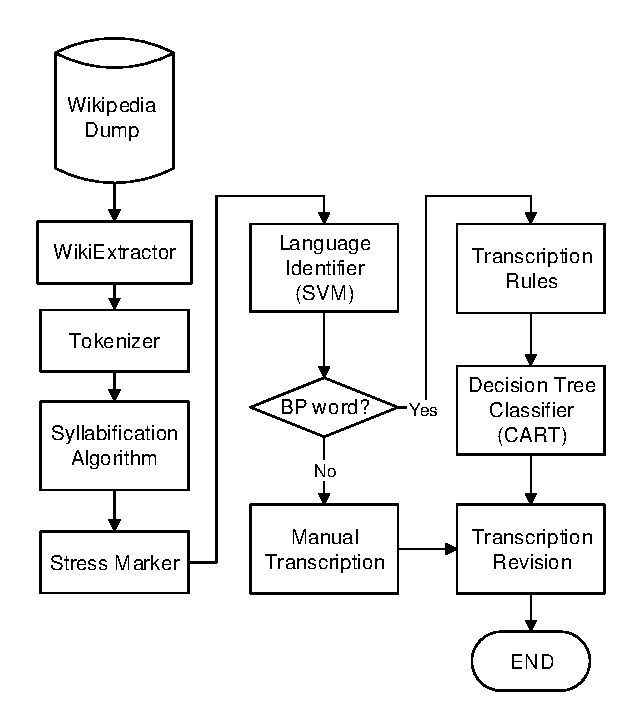
\includegraphics[width=8cm]{./gfx/flowchart_mod.pdf}}
\caption{{\it System architecture for building the pronunciation dictionary.}}
\label{g2p-architecture}
\end{figure}

We used the Portuguese Wikipedia's dump of 23\textsuperscript{rd} January 2014 as the primary word list for the pronunciation dictionary. In order to obtain plain text from the articles, we employed WikiExtractor \cite{Wikiextractor2013}; it strips all the  MediaWiki markups and metadata forms. Afterwards, texts were tokenized and unique words types extracted. The Portuguese Wikipedia has about 168,8 million word tokens and 9,7 million types, distributed among  820,000 articles. With the purpose of avoiding misspellings, URLs and other spurious data, only words with frequency higher than 10, which showed neither digits nor punctuation marks were selected. 

A Language Identifier module was developed in order to detect loanwords in the pronunciation dictionary. The Identifier consists of a Linear Support Vector Machine Classifier \cite{Steinwart2008} and was implemented in Python, through Scikit-learn \cite{Scikit2011}. It was trained on a corpus made of the 200,000, containing 100,000 Brazilian Portuguese words and 20,000 words of each of the following languages: English, French, German, Italian and Spanish. All of these words were collected through web crawling News' sites and were not revised. We selected these languages because they are the major donors of loanwords to Brazilian Portuguese \cite{Alves2001}. From these words we extracted features such as initial and final bi- and trigraphs;  number of accented graphs, vowel-consonant ratio; average mono-, bi- and trigraphs probability; and used them to estimate the classifier. Further details can be found in the website of the Project\footnote{http://nilc.icmc.usp.br/listener/aeiouado}. After training, we applied the classifier to the Wikipedia word list with the purpose of identifying loanwords among data. The identified loanwords were then separated from the rest of words for later revision, i.e. they were not submitted to automatic transcription.

Our syllabification algorithm follows a rule-approach and is based straightforwardly on the syllabification rules described in the Portuguese Language Orthographic Agreement \cite{Acordo2009}. Given space limitations, rules were omitted from this paper as they can be found in the website of the project, along with all the resources developed for the dictionary. As for the stress marker, once the syllable structure is known in Brazilian Portuguese, one can predict where stress falls. Stress falls:

\begin{enumerate}
 \item on the antepenultimate syllable if it has an accented vowel $<$\'a,\^a,\'e,\^e,\'i,\'o,\^o,\'u$>$;
 \item on the ultimate syllable if it contains the accented vowels $<$\'a,\'e,\'o$>$ or $<$i,u$>$; or if it ends with one of the following consonants $<$r,x,n,l,z$>$;
 \item on the penultimate syllable otherwise.
\end{enumerate}

The transcriber is based on a hybrid approach, making use of manual transcription rules and an automatic classifier, which builds Decision Trees. Initially, transcription rules are applied to the words. The rules covers not all possible graphemes to phoneme relations, but only those which are predictable by context. The output of the rules is what we called the intermediary transcription form. After obtaining it, a machine learning classifier is applied in order to predict the transcription of the remaining graphemes. Figure 2 gives an example of the transcription process.

\begin{figure}[!ht]
\centerline{ 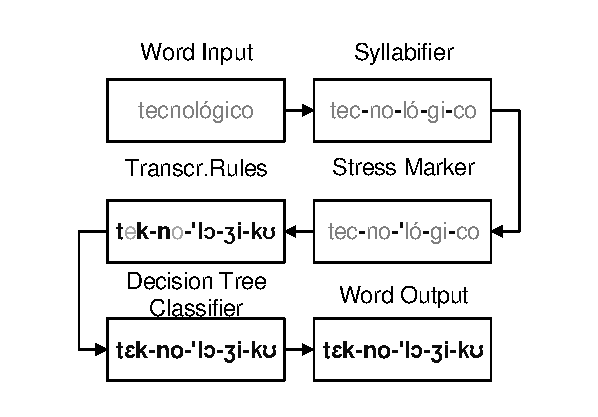
\includegraphics[width=8cm]{./gfx/transcript_ex.pdf}}
\caption{{\it Example of the transcription procedure -- in grey: graphemes yet to be transcribed; in black: graphemes already transcribed.}}
\label{transcExample}
\end{figure}

The rules' phase has two main goals: guarantee the correct transcription of certain predictable graphemes (mostly consonants) and also ensure the alignment between graphemes and phones for the classifier. They were set in order to avoid overlapping and order conflicts. Long sequences of graphemes, such as triphthongs, contextual diphthongs and general diphthongs are transcribed first (e.g.  $<$x-ce$> \rightarrow $\textipa{[-se]}). Then graphemes involving phones that undergo phonological processes are transcribed (e.g. $<$ti$> \rightarrow $\textipa{[tSi]}, $<$di$> \rightarrow $\textipa{[dZi]}). After that, several contextual and general monophones are transcribed (e.g. $<$\#x$> \rightarrow $\textipa{[S]}, $<$\#e-x$> \rightarrow $\textipa{[}\#\textipa{e-z]}). 

On what regards to the classifier, it was developed primarily to deal with the transcription of vowels. In Brazilian Portuguese, vowels have a very irregular behavior, specially the mid ones. Therefore the relations between the vowels' graphemes and their corresponding phonemes are hard to predict beforehand through rules. Consider, for instance, the words ``teto'' \emph{(roof)} and ``gueto'' \emph{(ghetto)}; both are nouns and share basically the same orthographic environment. However the former is pronounced with an open ``e'' \textipa{["tE.tU]} and the latter with a closed one \textipa{["ge.tU]}. The classifier employs Decision Trees, through an optimised version of the CART (Classification and Regression Trees) algorithm and was implemented in Python, by means of the Scikit-learn library \cite{Scikit2011}. 

The algorithm was trained over a corpus of 3,500 words phonetically transcribed and manually revised, with a total of 39,934 instances of phones. The feature extraction happened in the following way. After reviewing the data, we obtained the intermediary transcription form for each of these words and aligned them with the manual transcription. Then, we split the intermediary transcription form into its corresponding phones and, for each phone, we extracted the following information: 

\begin{enumerate}
 \item the phone itself; 
 \item 8 previous phones; 
 \item 8 following phones; 
 \item the distance between the phone and the tonic syllable; 
 \item word class -- parts of speech; 
 \item the manually transcribed phone. 
\end{enumerate}

We considered a window of 8 phones in order deal with vowel harmony phenomena. By establishing a window with such length, one  can assure that pretonic phones will be able to reach the transcription of the vowels in the stressed syllable. The classifier was applied to all 108,389 words categorized as BP words by the Language Identifier module, all of them were cross-checked by two linguists with experience in Phonetics and Phonology.

The Portuguese Wikipedia has about 168,8 million word tokens and 9,7 million types, distributed among 820k articles. After applying the filters to the data, i.e. words with frequency higher than 10, with no digits nor punctuation marks, we ended up with circa 238k word types, representing 151,9 million tokens. Table 1 describes the data.

\begin{table} [t,h]
\caption{\label{wikipedia} {\it Portuguese Wikipedia Summary -- Dumped on 23\textsuperscript{rd} January 2014.}}
\vspace{2mm}
\centerline{
\begin{tabular}{ccc}
\hline \bf & \bf Word Tokens  & \bf Word Types\\\hline
Wikipedia & 168,823,100 & 9,688,039 \\
Selected  & 151,911,350 & 238,012 \\
\textbf{\% Used} &90.0 & 2.4 \\
\hline
\end{tabular}}
\end{table}

The selected words covers 90,0\% of the Wikipedia content. Although the number of selected word types seems too small at first glance, one of the reasons is that 7,901,277 of the discarded words were numbers (81,5\%). The remaining discarded words contained misspellings (\emph{dirijem-se} -- it should be \emph{dirigem-se}), used a non-Roman alphabet ($\lambda$\emph{\'o}$\gamma \omega$), were proper names (\emph{Stolichno}, \emph{Z\'e-pereira}), scientific names (\emph{Aegyptophitecus}), abbreviations or acronyms (LCD, HDMI). 

As for the language identifier, we trained and evaluated it with the 200,000 words multilingual corpus. The corpus consists of 100,000 Brazilian Portuguese words and 20,000 words from each of the following languages: English, French, German, Italian and Spanish. All of these words were collected through web crawling News' sites and were not revised. The results obtained for the identifier, through 5-fold cross validation are described in Table 2. 

\begin{table} [t,h]
\caption{\label{langIdentEval} {\it Results from the Language Identifier module -- Training Phase.}}
\vspace{2mm}
\centerline{
\begin{tabular}{ccccc}
\hline
 & \textbf{Precision} & \textbf{Recall} & \textbf{F1-score} & \textbf{Support} \\ \hline
BP words & 0.85 & 0.89 & 0.87 & 100,000 \\ 
Foreign Words & 0.88 & 0.84 & 0.86 & 100,000 \\
\bf Avg/Total & 0.86 & 0.86 & 0.86 & 200,000 \\ \hline
\end{tabular}}
\end{table}

The language identifier showed an average F1-score of 0.86. Although such result is not as good as we expected -- some authors reported 99\% by using similar methods with trigrams probability, the relatively low F1-score can be explained given the nature of the data. In most language identifiers, the input  consists of texts or several sentences, in other words, there is much more data available for the classifier. Since we are working with single words, the confusion of the model is higher and the results are, consequently, worse. Additionally, because the word list used to train the identifier was not revised, there is noise among the data. After training and evaluating the classifier, we applied it to the selected word list derived from the Wikipedia, in order to detect loanwords. Table 3 describes the results gathered.

\begin{table} [t,h]
\caption{\label{langIdentWiki} {\it Results from the Language Identifier module -- Wikipedia word list.}}
\vspace{2mm}
\centerline{
\begin{tabular}{cc}
\hline
 & \textbf{Wikipedia word list}\\ \hline
BP words & 108,370 (46\%)\\ 
Foreign Words & 129,642 (54\%)\\
\bf Total & 238,012 \\ \hline
\end{tabular}}
\end{table}

As one can observe, although we established a frequency filter to avoid spurious words, many loanwords still remain. More than half of the word list selected from Wikipedia consists of foreign words. Notwithstanding that, the list of Brazilian Portuguese words is still of considerable size. For instance, the CMUdict \cite{CMUdict1998}, a reference pronunciation dictionary for the English language, has about 125,000 word types.

Concerning the syllabification algorithm and the stress marker, we did not evaluate them in isolation, but together with the transcriber since the rules for each of these modules are intertwined. That is to say the transcription rules are strictly dependent on the stress marker module and the syllable identifier. Besides, the Decision Tree Classifier is built upon the output of the transcription rules, so it is entirely dependent on it. The Decision Tree Classifier was trained over a corpus of 3,500 cross-checked transcribed words, containing 39,934 instances of phones. We analyzed its performance through 5-fold cross validation, the results for each individual phone are summarized in Table 4.

\begin{table} [t,!h]
\caption{\label{transcriberEval} {\it Results from the Transcriber -- Performance per phone.}}
\vspace{2mm}
\centerline{
\begin{tabular}{ccccc}
\hline
 & \bf Precision & \bf Recall & \bf F1-score & \bf Support \\ \hline
\emph{syl. boundary} & 1.00 & 1.00 & 1.00 & 9099 \\ 
\emph{stress} & 1.00 & 1.00 & 1.00 & 3507 \\ 
\textipa{p} & 1.00 & 1.00 & 1.00 & 760 \\ 
\textipa{b} & 1.00 & 1.00 & 1.00 & 357 \\ 
\textipa{t} & 0.99 & 0.99 & 0.99 & 1135 \\ 
\textipa{d} & 0.99 & 0.99 & 0.99 & 1148 \\ 
\textipa{k} & 0.99 & 0.99 & 0.99 & 978 \\ 
\textipa{g} & 1.00 & 1.00 & 1.00 & 298 \\ 
\textipa{tS} & 0.98 & 0.98 & 0.97 & 450 \\ 
\textipa{dZ} & 0.96 & 0.96 & 0.96 & 243 \\ 
\textipa{m} & 1.00 & 1.00 & 1.00 & 668 \\ 
\textipa{n} & 1.00 & 1.00 & 1.00 & 556 \\ 
\textipa{\textltailn} & 1.00 & 1.00 & 1.00 & 69 \\ 
\textipa{f} & 1.00 & 1.00 & 1.00 & 311 \\ 
\textipa{v} & 1.00 & 1.00 & 1.00 & 531 \\ 
\textipa{s} & 0.98 & 0.98 & 0.98 & 2309 \\ 
\textipa{z} & 0.93 & 0.94 & 0.93 & 416 \\ 
\textipa{S} & 0.84 & 0.84 & 0.84 & 138 \\ 
\textipa{k.s} & 0.72 & 0.64 & 0.66 & 41 \\ 
\textipa{Z} & 1.00 & 1.00 & 1.00 & 196 \\ 
\textipa{l} & 1.00 & 1.00 & 1.00 & 682 \\ 
\textipa{L} & 1.00 & 1.00 & 1.00 & 58 \\ 
\textipa{R} & 1.00 & 1.00 & 1.00 & 1388 \\ 
\textipa{h} & 0.98 & 0.99 & 0.99 & 737 \\ 
\textipa{H} & 0.97 & 0.92 & 0.94 & 169 \\ 
\textipa{w} & 0.97 & 0.98 & 0.97 & 441 \\ 
\textipa{\~w} & 0.98 & 0.99 & 0.99 & 309 \\ 
\textipa{j} & 0.97 & 0.95 & 0.96 & 223 \\ 
\textipa{\~j} & 0.95 & 1.00 & 0.98 & 110 \\ 
\textipa{a} & 1.00 & 1.00 & 0.99 & 2316 \\ 
\textipa{@} & 0.99 & 0.99 & 0.99 & 1093 \\ 
\textipa{E} & 0.65 & 0.68 & 0.66 & 275 \\ 
\textipa{e} & 0.93 & 0.91 & 0.92 & 1779 \\ 
\textipa{i} & 0.98 & 0.99 & 0.98 & 2073 \\ 
\textipa{I} & 0.97 & 0.97 & 0.97 & 365 \\ 
\textipa{O} & 0.69 & 0.75 & 0.71 & 220 \\ 
\textipa{o} & 0.93 & 0.92 & 0.93 & 1112 \\ 
\textipa{u} & 0.96 & 0.96 & 0.96 & 488 \\ 
\textipa{U} & 1.00 & 1.00 & 1.00 & 1033 \\ 
\textipa{\~a} & 1.00 & 1.00 & 1.00 & 719 \\ 
\textipa{\~e} & 0.96 & 0.97 & 0.97 & 497 \\ 
\textipa{\~i} & 0.99 & 0.99 & 0.99 & 274 \\ 
\textipa{\~o} & 0.97 & 0.96 & 0.97 & 299 \\ 
\textipa{\~u} & 0.94 & 0.92 & 0.93 & 64 \\ 
Avg/Total & 0.98 & 0.98 & 0.98 & 39934 \\ \hline
\end{tabular}}
\end{table}

As it can be seen, the method achieved very good results, with a F1-score of 0.98. Many segments were transcribed with 100\% accuracy, most of them were consonants. As it was expected, the worst results are related to mid vowels \textipa{[E, e, O, o]}, specially mid-low vowels, \textipa{[E]} showed a F1-score 0.66 and \textipa{[O]} of 0.71. It can be the case that since the grapheme context is the same for \textipa{[E, e]} and \textipa{[O, o]}, the DecisionTree classifier generalizes, in some cases, to the most frequent phone, that is the mid-high vowels \textipa{[e,o]}. The transcriber also had problems with the \textipa{[k.s]} (F1-score: 0.66) and \textipa{[S]} (F1-score: 0.84). This result was also expected, both these phones are related to the grapheme $<$x$>$ which, in Brazilian Portuguese, shows a very irregular behavior. In fact, $<$x$>$ can be pronounced as \textipa{[S, s, z, k.s]}, depending on the  word:  ``bruxa'' \emph{(witch)} \textipa{[S]}, ``pr\'oximo'' \emph{(near)} \textipa{[s]};  ``exame'' \emph{(test)} \textipa{[z]} and ``axila'' \emph{(armpit)} \textipa{[k.s]}.

We presented the method we employed in building a pronunciation dictionary for Brazilian Portuguese. High F1-score values were achieved while transcribing most of the graphemes in Brazilian Portuguese and the dictionary can be considered robust enough for Large Vocabulary Continuous Speech Recognition (LVCSR) and Speech Synthesis. Although the rules we developed are language-specific, the architecture we used for compiling the dictionary, by using transcription rules and machine learning classifiers, can be successfully replicated in other languages. In addition, the entire dictionary, all scripts, algorithms and corpora were made publicly available.\footnote{\url{http://nilc.icmc.usp.br/aeiouado}}\footnote{\url{https://github.com/gustavoauma/aeiouado_g2p}}

\paragraph{Further developments}

Since the publishing date of our paper (\citeauthor{Mendonca2014}~\cite{Mendonca2014}), Aeiouad\^o \ac{G2P} has been improved. Recently, we increased the training database to XXX words (XXX phone tokens). Moreover we are now using extra morphological information in order to determine the grapheme's transcription, mostly to solve the problems with the mid vowels \textipa{[E, e, O, o]}. 

Previously we were using only the parts of speech as the source of morphological information. We assumed that by just providing the words' parts of speech, the Decision Tree Classifier would be able to learn and differ pairs of heterophonic homographs, such as ``jogo'' \textsc{noun} \emph{(game)} and ``jogo'' \textsc{verb} \emph{(I play)}, or ``governo'' \textsc{noun} \emph{(government)} and ``governo'' \textsc{verb} \emph{(I rule)}. However, given the poor performance of the conversor in discerning between \textipa{[E]} vs. \textipa{[e]}, and \textipa{[O]} vs. \textipa{[o]}; we decided to refine the morphological features. 

We adapted the training database to the Unitex-PB dictionary \cite{Muniz2004}, which follows  formalismo DELA (Dictionnarie Electronique du LADL)

There is a huge lexicon with,

This type of alternation is very productive in \ac{BP}.  reported to have collected 1,812 pairs of heterophonic homographs in dictionaries and , although only 226 occurred in corpus).

\citeauthor{}, Pandu , although in a corpus analysis, only 226 \cite{Shulby2013}.

However this is not the case. Previously, only the word class information was used to determine. We thought that would be enough to 

\section{Speech Corpora}
Lorem ipsum quod dolor sit amet.

\subsection{TIMIT}
Lorem ipsum quod dolor sit amet.

\subsection{WSJ0}
The CSR-I WSJ0 corpus was compiled by \citeauthor{Garofolo1993} \cite{Garofolo1993}, within the 
DARPA Spoken Language Program in order to support research on large-vocabulary \ac{CSR} systems.

It focuses on American English and contains read speech of texts drawn from a corpus with Wall 
Street Journal articles. The texts to be read were selected to fall within either a 5,000-word or 
a 20,000-word subset of the WSJ text corpus. All verbal punctuation is read out aloud and the 
prompting texts have been pre-filtered to insure unambiguous pronunciations of words. The corpus 
comprises spontaneous dictation by journalists with varying degrees of experience in dictation, 
the precise number of speakers is informed in the documentation. As for the recording environment, 
a Sennheiser close-talking head-mounted microphone was used together with a secondary microphone of 
varying types.  

\autoref{tab:wsj0-summary} describes a summary of the WSJ0 corpus.

\begin{table}[!htb]
\caption[Summary of the entire WSJ0 Corpus.]{Summary of the entire WSJ0 Corpus.}
\smallskip
\centering
\begin{tabular}{ccc} \toprule
  Recorded files & X \\
  Total speech time & X \\
  Average time per file & X \\
  Original format & X \\
  Number of different speakers & X \\
  \bottomrule
\end{tabular}
\label{tab:wsj0-summary}
\end{table}

For building the acoustic model, we decided to use only a portion of the WSJ0. This decision was made 
since a considerable number of files in the WSJ recordings had:

\begin{enumerate}
 \item disfluencies phenomena, such as mispronunciations, verbal deletions, false starts and spoken word fragments; 
 \item emphatic stress in words which would normally not be stressed due to lexical or syntactic factors;
 \item non-speech events (chair squeak, cross talk, door slams, paper rustle, phone ring, etc.)
 \item truncated audio files.
\end{enumerate}

All these recordings would degrade the estimation of the acoustic model, giving rise to poor phone or 
triphone \ac{HMM}s. On account of this problem, we excluded all these files from the training process.

After that, to check the consistency of the transcription, we used forced alignment with an acoustic
monophone model trained over all other English corpora. Forced alignment was performed through 
a general-purpose Viterbi recognizer, which employed beam search to find the most likely \ac{HMM} states 
for an utterance. The beam-width was set to 250. That is, for each audio file, if the transcription provided 
did not correspond to any alignment found by expanding each node over the best 250 hypotheses, 
the file was pruned and not considered for training.




The portion of the WSJ0 that we used is detailed in \autoref{tab:wsj0-used-summary}

\begin{table}[!htb]
\caption[Summary of WSJ0 Part We Used.]{Summary of WSJ0 Part We Used.}
\smallskip
\centering
\begin{tabular}{ccc} \toprule
  Recorded files & X \\
  Total speech time & X \\
  Average time per file & X \\
  Original format & X \\
  Number of different speakers & X \\
  \bottomrule
\end{tabular}
\label{tab:wsj0-used-summary}
\end{table}


\subsection{SpeechDat}
Lorem ipsum quod dolor sit amet.

\subsection{Listener's Corpus}
Lorem ipsum quod dolor sit amet.

\begin{table}[!htb]
\caption[Summary of Listener's Corpus.]{Summary of the Listener's Corpus.}
\smallskip
\centering
\begin{tabular}{ccc} \toprule
  Recorded files & 6,892 \\
  Total speech time & ~6.8 hours \\
  Average time per file & 1.02 seconds \\
  Original format & WAV 16kHz \\
  Number of different speakers & 53 \\
  \bottomrule
\end{tabular}
\end{table}

\subsection{Oxford Dictionary AmE Corpus}
The Oxford Dictionary \ac{AmE} corpus was compiled by web crawling specially to this project. Oxford University Press
has been making dictionaries for the English language for more than 150 years. Their dictionaries are very traditional and widely 
known whether in lexicographers' or laymen's circles. Recently, they made the dictionaries publicly available
on the web\footnote{\url{http://www.oxforddictionaries.com/}}. For the \ac{AmE} version, one can browse $350,000$ words, definitions, 
and entries, together with over $600,000 synonyms$\footnote{\url{http://www.oxforddictionaries.com/words/content-help}}.
A word example can be found in \autoref{fig:oxford-example}.

\begin{figure}[!htb]
        \myfloatalign
        {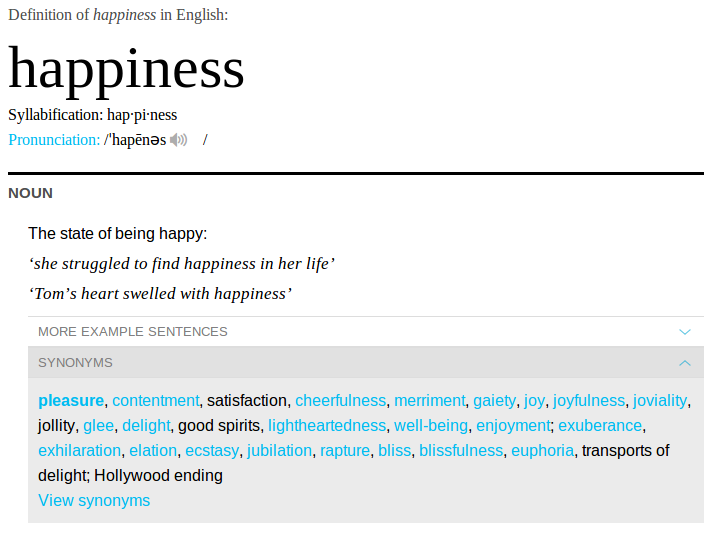
\includegraphics[width=.66\linewidth]{gfx/example-oxford-definition.png}}
        \caption{Entry example in the Oxford Dictionary online.}
        \label{fig:oxford-example}
\end{figure}

As one may notice in \autoref{fig:oxford-example}, the entry has many information: (i) the word itself, in ortographic form;
(ii) word syllabification; (iii) its pronunciation; (iv) the word audio file;
(v) \ac{POS} data; (vi) definition; (vii) some example sentences; (viii) and a list of synonyms. The pronunciation
follows Oxford's own transcription convention, which can be mapped on the \ac{IPA} as in \autoref{tab:oxford-dictionary-ipa}.

\renewcommand{\arraystretch}{0.8}% Tighter
\begin{table}[!htbp]
\caption[Oxford Dictionary phone convention.]{Oxford Dictionary phone convention.}
\smallskip
\centering
\begin{tabular}{ccccc} \toprule
\tableheadline{\#} & \tableheadline{Oxford Phone} & \tableheadline{IPA Phone} & \tableheadline{Example} & \tableheadline{Transcription} \\ \midrule
1 & (h)w & \textipa{aaaaa} & when & trans \\ 
2 & \"a & \textipa{O} & hot & trans \\ 
3 & \^o & \textipa{O} & saw & trans \\ 
4 & \={oo} & \textipa{u} & too & trans \\ 
5 & \=a & \textipa{eI} & day & trans \\ 
6 & \=e & \textipa{i} & see & trans \\ 
7 & \=i & \textipa{aI} & my & trans \\ 
8 & \=o & \textipa{oU} & no & trans \\ 
9 & \textipa{@} & \textipa{@} & ago & trans \\ 
10 & \textipa{\oe} (foreign) & \textipa{\oe} & Goethe (German) & trans \\ 
11 & \textipa{\u{oo}} & \textipa{U} & put & trans \\ 
12 & \textipa{Y} (foreign) & \textipa{Y} & Utrecht (French) & trans \\ 
13 & a & \textipa{\ae} & cat & trans \\ 
14 & b & \textipa{b} & bad & trans \\ 
15 & CH & \textipa{tS} & chip  & trans \\ 
16 & d & \textipa{d} & day & trans \\ 
17 & e & \textipa{E} & bed & trans \\ 
18 & e(\textipa{@})r & \textipa{Er} & hair & trans \\ 
19 & f & \textipa{f} & fight & trans \\ 
20 & g & \textipa{g} & get & trans \\ 
21 & h & \textipa{h} & hi & trans \\ 
22 & i & \textipa{I} & sit & trans \\ 
23 & i(\textipa{@})r & \textipa{ir} & near & trans \\ 
24 & j & \textipa{dZ} & jar & trans \\ 
25 & k & \textipa{k} & kick & trans \\ 
26 & KH & \textipa{x} & loch & trans \\ 
27 & l & \textipa{l} & lie & trans \\ 
28 & m & \textipa{m} & man & trans \\ 
29 & N (foreign) & \textipa{\~v} & bon (French) & trans \\ 
30 & n & \textipa{n} & no & trans \\ 
31 & NG & \textipa{n} & ring & trans \\ 
32 & oi & \textipa{OI} & boy & trans \\ 
33 & ou & \textipa{aU} & how & trans \\ 
34 & p & \textipa{p} & pie & trans \\ 
35 & r & \textipa{r} & run & trans \\ 
36 & s & \textipa{s} & save & trans \\ 
37 & SH & \textipa{S} & she & trans \\ 
38 & t & \textipa{t} & time & trans \\ 
39 & TH & \textipa{D} & this & trans \\ 
40 & TH & \textipa{T} & thin & trans \\ 
41 & v & \textipa{v} & vow & trans \\ 
42 & y & \textipa{y} & yes & trans \\ 
43 & z & \textipa{z} & zoo & trans \\ 
44 & ZH & \textipa{Z} & decision & trans \\
\bottomrule
\end{tabular}
\label{tab:oxford-dictionary-ipa}
\end{table}
\renewcommand{\arraystretch}{1.0}% Normal

For compiling the corpus, we built a spider through Scrapy \cite{Scrapy2014}, a web crawling framework for Python specially 
designed to crawl websites and extract structured data from their pages. In total, $49,263$ entries were crawled. This number 
was defined in order to be consonant with the dictionary's legal aspects, which defines that only a fraction of its
content might be downloaded either personal or institutional use. For each word, we crawled three fields: the word, its transcription 
and the audio file. According to Oxford University Press' legal notice, we may not display or distribute any of the crawled 
content in any media, nor we may use commercially. Therefore, we used the data only for estimating the parameters of the acoustic model.

Some xenophones, i.e. phones from other languages, might be seen in \autoref{tab:oxford-dictionary-ipa}. This happens because
Oxford Dictionary also register some loanwords (specially those coming from Frech) with their original pronunciation,
like ``Utrecht'' and ``bon''. Since our goal is to deal only with Brazilian-accented English, words such as these
were excluded, so no word among the $49,263$ entries contain xenophones.

Oxford Dictionary's were recorded by many speakers (both male and female), with high-quality microphones, in sound-isolation rooms.
The audios are saved in MP3 format with \ac{VBR}, for this reason we had convert each file into WAV and downsample them to $16$ kHz.
The quality of the audio is excelent with a very high \ac{SNR}, as can be seen in the spectrogram for the word ``happiness'' 
in \autoref{fig:spectrogram-happiness}.

\begin{figure}[!htb]
        \myfloatalign
        {\includegraphics[width=.66\linewidth]{gfx/oxford-spectrogram-happiness.png}}
        \caption{Spectrogram of the word ``happiness'', present in the Oxford Dictionary AmE Corpus.}
        \label{fig:spectrogram-happiness}
\end{figure}

As one may observe in the regions of silence at the beginning and at the end of the utterance, the background noise approaches to zero.
A summary of the corpus can be seen in \autoref{fig:spectrogram-happiness}.

\begin{table}[!htb]
\caption[Summary of the Oxford Dictionary AmE Corpus.]{Summary of the Oxford Dictionary AmE Corpus.}
\smallskip
\centering
\begin{tabular}{ccc} \toprule
  Recorded files & 49,263 \\
  Total speech time & ~4 hours \\
  Average time per file & 1.02 seconds \\
  Original format & MP3 (VBR) \\
  Number of different speakers & Unknown \\
  \bottomrule
\end{tabular}
\label{tab:oxford-summary}
\end{table}

\subsection{Cambridge Dictionary}
Lorem ipsum quod dolor sit amet.

\subsection{OGI-22}
Lorem ipsum quod dolor sit amet.

\subsection{Westpoint}
Lorem ipsum quod dolor sit amet.

\subsection{LapsBM}
Lorem ipsum quod dolor sit amet.

\subsection{Youtube}
Lorem ipsum quod dolor sit amet.

\begin{table}[!htb]
\caption[Summary of Listener's Corpus.]{Summary of the Listener's Corpus.}
\smallskip
\centering
\begin{tabular}{ccc} \toprule
  Recorded files & 6,892 \\
  Total speech time & ~6.8 hours \\
  Average time per file & 1.02 seconds \\
  Original format & WAV 16kHz \\
  Number of different speakers & 53 \\
  \bottomrule
\end{tabular}
\end{table}


\section{Building the Acoustic Model}

\subsection{The Phoneset}\label{sec:listener-phoneset}

Since our goal is to build an \ac{ASR} system capable of recognizing non-native speech, we propose
to use an interlingual phoneset as the basis of the pronunciation model. By doing this, we can define
\ac{HMM} models for estimating phones which are part of both the speaker's native language (\ac{BP}) and 
the target language (\ac{AmE}).

A straightforward approach would be to look up the literature in phonetics and phonology in order to find
a \ac{BP}--\ac{AmE} interlingual phoneset. However, to the best of our knowledge, no previous works were carried 
out in this regard. There are papers addressing specific mispronunciations, such as those discussed in \autoref{sec:common-mispronunciation}, 
which list some occurring interlingual phones, but there is not a wide-ranging study available about this matter.

Therein we had to develop our own interlingual phoneset. For simplicity, we decided to adapt the union set formed 
by the phones contained in two machine-readable dictionaries, one for \ac{AmE}: \ac{CMUdict} \cite{CMU2008}, and another for \ac{BP}: 
Aeiouad\^o \cite{Mendonca2014}. By doing this, we can cover most of the phone productions that brazilian \ac{ESL} learners are likely
to make. Advanced students will tend to use more properly the English phones, whereas beginners will have a stronger accent,
thus producing more phones from the \ac{BP} phoneset. A brief description of each of these dictionaries is given below, before 
we go into further details of our interlingual set.

\ac{CMUdict} \citep{CMU2008} is a machine-readable pronunciation dictionary for \ac{AmE} which has about $125,000$ 
words and their transcriptions. It was designed primarily for speech applications, such as speech recognition and synthesis, 
and it has been widely tested in both Academia and industry.

Words in \ac{CMUdict} are transcribed using ARPAbet, a phonetic transcription code developed by the Advanced Research Projects Agency in 
$1971$. It represents each \ac{AmE} phone with a distinct sequence of \ac{ASCII} characters. In the dictionary, there are in total $39$ 
phones plus stress marks. The phone convention is described on \autoref{tab:cmu-conv}.

\renewcommand{\arraystretch}{0.95}% Tighter
\begin{table}[p]
\caption[CMUdict phone convention.]{CMUdict phone convention.}
\smallskip
\centering
\begin{tabular}{ccccc} \toprule
\tableheadline{\#} & \tableheadline{CMU Phone} & \tableheadline{IPA Phone} & \tableheadline{Example} & \tableheadline{Transcription} \\ \midrule
1 & AA & [\textipa{A}] & odd & AA D \\
2 & AE & [\textipa{\ae}] & at & AE T \\
3 & AH & [\textipa{@}] & hut & HH AH T \\
4 & AO & [\textipa{O}] & ought & AO T \\
5 & AW & [\textipa{aU}] & cow & K AW \\
6 & AY & [\textipa{aI}] & hide & HH AY D \\
7 & B & [\textipa{b}] & be & B IY \\
8 & CH & [\textipa{tS}] & cheese & CH IY Z \\
9 & D & [\textipa{d}] & dee & D IY \\
10 & DH & [\textipa{D}] & thee & DH IY \\
11 & EH & [\textipa{E}] & Ed & EH D \\
12 & ER & [\textipa{@r}] & hurt & HH ER T \\
13 & EY & [\textipa{A\*r}] & ate & EY T \\
14 & F & [\textipa{f}] & fee & F IY \\
15 & G & [\textipa{g}] & green & G R IY N \\
16 & HH & [\textipa{h}] & he & HH IY \\
17 & IH & [\textipa{I}] & it & IH T \\
18 & IY & [\textipa{i}] & eat & IY T \\
19 & JH & [\textipa{dZ}] & gee & JH IY \\
20 & K & [\textipa{k}] & key & K IY \\
21 & L & [\textipa{l}] & lee & L IY \\
22 & M & [\textipa{m}] & me & M IY \\
23 & N & [\textipa{n}] & knee & N IY \\
24 & NG & [\textipa{N}] & ping & P IH NG \\
25 & OW & [\textipa{oU}] & oat & OW T \\
26 & OY & [\textipa{OI}] & toy & T OY \\
27 & P & [\textipa{p}] & pee & P IY \\
28 & R & [\textipa{\*r}] & read & R IY D \\
29 & S & [\textipa{s}] & sea & S IY \\
30 & SH & [\textipa{S}] & she & SH IY \\
31 & T & [\textipa{t}] & tea & T IY \\
32 & TH & [\textipa{T}] & theta & TH EY T AH \\
33 & UH & [\textipa{U}] & hood & HH UH D \\
34 & UW & [\textipa{u}] & two & T UW \\
35 & V & [\textipa{v}] & vee & V IY \\
36 & W & [\textipa{w}] & we & W IY \\
37 & Y & [\textipa{y}] & yield & Y IY L D \\
38 & Z & [\textipa{z}] & zee & Z IY \\
39 & ZH & [\textipa{Z}] & seizure & S IY ZH ER \\
\bottomrule
\end{tabular}
\label{tab:cmu-conv}
\end{table}
\renewcommand{\arraystretch}{1.0}% Normal

As for Aeiouad\^o, as described in Section~\autoref{sec:aeiouado}, its transcriptions are
based on the dialect of S\~ao Paulo city and contains 39 different phones. The dictionary makes
use of a hybrid approach for converting graphemes into phonemes, 
which employs both manual transcription rules and machine learning algorithms. Its phone convention
is presented in Table~\autoref{tab:aeiouado-conv}.

\renewcommand{\arraystretch}{0.9}% Tighter
\begin{table}[p]
\caption[Aeiouad\^o phone convention.]{Aeiouad\^o phone convention.}
\smallskip
\centering
\begin{tabular}{ccccc} \toprule
\tableheadline{\#} & \tableheadline{Aeiouad\^o Phone} & \tableheadline{IPA Phone} & \tableheadline{Example} & \tableheadline{Transcription} \\ \midrule
1 & a & [\textipa{a}] & amor & a m o x \\
2 & a$\sim$ & [\textipa{\~a}] & canto & k a$\sim$ t U \\
3 & b & [\textipa{b}] & besta & b e s t @ \\
4 & d & [\textipa{d}] & da & d a \\
5 & dZ & [\textipa{dZ}] & dia & dZ i @ \\
6 & E & [\textipa{E}] & \'e & E \\
7 & e & [\textipa{e}] & dedo & d e d U \\
8 & e$\sim$ & [\textipa{\~e}] & venda & v e$\sim$ d @ \\
9 & f & [\textipa{f}] & frio & f 4 i U \\
10 & g & [\textipa{g}] & gula & g u l @  \\
11 & G & [\textipa{G}] & carga & carga \\
12 & i & [\textipa{i}] & a\'i & a i \\
13 & I & [\textipa{I}] & come & k o$\sim$ m I \\
14 & i$\sim$ & [\textipa{\~i}] & sim & s i$\sim$ \\
15 & J & [\textipa{\textltailn}] & ganho & g a$\sim$ J U \\
16 & j & [\textipa{y}] & pai & p a j \\
17 & j$\sim$ & [\textipa{\~y}] & parem & p a 4 e$\sim$ j$\sim$ \\
18 & k & [\textipa{k}] & compra & k o$\sim$ p 4 @ \\
19 & l & [\textipa{l}] & l\'a & l a \\
20 & L & [\textipa{L}] & palha & p a L @ \\
21 & m & [\textipa{m}] & m\~ae & m a$\sim$ j$\sim$ \\
22 & n & [\textipa{n}] & n\~ao & n a$\sim$ w$\sim$ \\
23 & O & [\textipa{O}] & p\'o & p O \\
24 & o & [\textipa{o}] & gorro & g o x U \\
25 & o$\sim$ & [\textipa{\~o}] & com & k o$\sim$ \\
26 & p & [\textipa{p}] & pessoa & p e s o @ \\
27 & s & [\textipa{s}] & susto & s u s t U \\
28 & s & [\textipa{S}] & chato & S a t U \\
29 & t & [\textipa{t}] & tato & t a t U \\
30 & tS & [\textipa{tS}] & noite & n o j tS I \\
31 & u & [\textipa{u}] & durmo & d u G m U \\
32 & U & [\textipa{U}] & c\'umulo & k u m u l U \\
33 & u$\sim$ & [\textipa{\~u}] & um & u$\sim$ \\
34 & v & [\textipa{v}] & vida & v i d @ \\
35 & w & [\textipa{w}] & aula & a w l @ \\
36 & w$\sim$ & [\textipa{\~w}] & canh\~ao & k a$\sim$ J a$\sim$ w$\sim$ \\
37 & x & [\textipa{x}] & rato & x a t U \\
38 & z & [\textipa{z}] & zebra & z e b 4 @ \\
39 & 4 & [\textipa{R}] & arara & a 4 a 4 @ \\
40 & @ & [\textipa{@}] & bola & b O l @ \\
\bottomrule
\end{tabular}
\label{tab:aeiouado-conv}
\end{table}
\renewcommand{\arraystretch}{1.0}% Normal

In what concerns to our interlingual phoneset, we kept all \ac{CMUdict} phones, since that is the target language's
phoneset the learners are trying to achieve. Then we compared each phone in \ac{CMUdict} with those contained in 
Aieouad\^o, in order to check for missing phones and to analyze whether the overlapping ones really correspond to the same
sound.

At a first glance, it seems that \ac{BP} and \ac{AmE} share a pool of 24 common phones, comprising fifteen consonantes
[\textipa{b}, \textipa{d}, \textipa{dZ}, \textipa{f}, \textipa{g}, 
\textipa{k}, \textipa{l}, \textipa{m}, \textipa{n}, \textipa{p}, \textipa{s}, \textipa{S}, \textipa{t}, \textipa{tS}, \textipa{v}, \textipa{z}];
seven vowels [\textipa{E}, \textipa{i}, \textipa{I}, \textipa{O}, \textipa{u}, \textipa{U}, \textipa{@}];
together with two glides [\textipa{y}, \textipa{w}]. However it is worth noticing that this first impression does not
hold true. 

Despite the fact that both dictionaries present \ac{IPA} correspondences, such correspondes should not be taken
for granted, without previous analysis. In theory, \ac{IPA} is capable of describing any sound produced by the human vocal 
tract with exactness. Still \ac{IPA} transcriptions are biased by the level of detail one wishes to express and by the 
assumptions of the transcriber. This is the case for some of these overlapping phones. Several of these consonants and vowels, 
although marked with the same \ac{IPA} symbol by \ac{CMUdict} and Aeiouad\^o,
in fact, can not be regarded as being the same sound, since they show a very different distribution
in English and \ac{BP}. 

For instance, the production of /\textipa{p}, \textipa{t}, \textipa{k}/, 
in \ac{BP} and \ac{AmE} can be quite different. In English, such consonants are generally produced as 
[\textipa{p}, \textipa{t}, \textipa{k}]. However it is known that when they occur in certain contexts, 
for example, in word initial position or onset of a stressed syllable, they become aspirated; whence
[\textipa{p\super h}, \textipa{t\super h}, \textipa{k\super h}] \citep{Lisker1985}. 
On the other hand, this process is not found in \ac{BP}, where, disregard of the context, [\textipa{p}, \textipa{t}, \textipa{k}] show no 
relevant levels of aspiration \citep{Klein1999}. 

For that reason, in order to properly estimate the \ac{HMM} states for the interlingual phones, it is mandatory
to create aspirated phone models for these consonants that are different from the non-aspirated ones. In our interlingual
phoneset, we decided to keep the distinction between aspirated and non-aspirated phones. Therefore, according to our
convention, the /\textipa{p}/ that occurs in a stressed syllable of an English word like ``pie'' is transcribed as [\textipa{p\super h}], 
while the /\textipa{p}/ of an unstressed syllable or a BP word is transcribed as [\textipa{p}]. 

Additionally, some vowels that are described by both dictionaries with the same \ac{IPA} symbol are not exactly equal.
Although English and \ac{BP} both possess the vowels [\textipa{I, @, U}], the distribution
of these phones between both languages is fairly different. In \ac{AmE} such vowels hold phonological status, i.e. they 
are phonemes, so that one could find minimal pairs differing only by [\textipa{I, @, U}], such as ``sheep'' [\textipa{"Sip}] vs. 
``ship'' [\textipa{"SIp}]; ``cut'' [\textipa{"k\super h@t}] vs. ``cat'' [\textipa{"k\super h\ae t}]; and ``pull'' 
[\textipa{"p\super hUl}] vs. pool [\textipa{"p\super hul}]. As for \ac{BP}, these vowels exist solely as part
of a phonological process. When the tense vowels [\textipa{i, a, u}] occur in unstressed word-final position, they undergo a lenition process
and are produced as the lax vowels [\textipa{I, @, U}], respectivelly. Hence the \ac{BP} [\textipa{I, @, U}] have 
different formant values \cite{Fails1992} and all the typical characteristics of lax vowels, that is, they are short, 
they have less energy and, consequently, less clear-cut formants \cite{Nobre1987}.

With regard to the missing phones, there were 15 phones which are only present in the \ac{BP} inventory, these include eight vowels
[\textipa{a}, \textipa{\~a}, \textipa{e}, \textipa{\~e}, \textipa{\~i}, \textipa{o}, \textipa{\~o}, \textipa{\~u}]; five
consonants [\textipa{G}, \textipa{\textltailn}, \textipa{L}, \textipa{x}, \textipa{R}]; and two nasal glides
[\textipa{\~y}, \textipa{\~w}]. 

All eight vowels were added to the interlingual phoneset, for they encompass negative transfer problems. For instance, 
[\textipa{\~a}, \textipa{\~e}, \textipa{\~i}, \textipa{\~o}, \textipa{\~u}] are related to
vocalization of final nasals (\emph{vide} \ref{sec:voc-nasals}) and [\textipa{a}, \textipa{e}, \textipa{o}] to vowel assimilation (\emph{vide} \ref{sec:voc-assimilation}).

The \ac{BP} rhotic consonants [\textipa{R}, \textipa{G}, \textipa{x}], were merged onto the same sound, [\textipa{h}] owing to the fact
they they represent \ac{BP} dialectal variants not relevant to L1-L2 interphonology.

Furthermore, the \ac{BP} palatal consonants [\textipa{\textltailn}, \textipa{L}] were not considered in the final interlingual phoneset,
since we could not find, in the literature, any negative transfer process in which they occur. 

The nasal glides were excluded from the interlingual phoneset, instead we preffered to combine them with their accompanying vowels, in
order to create nasal diphthongs, such as [\textipa{\~a\~I}, \textipa{\~a\~U}, \textipa{\~e\~I}, \textipa{\~o\~I}]. This decision was 
made in accordance with \cite{Demasi2010}, which found that \ac{BP} nasal diphthongs have a very particular behavior, with 
articulatory, acoustic and aerodynamic patterns different from the non-nasalized ones. 
We believe that a single \ac{HMM} model for each diphthong will be able to better gauge this behavior.

The final phoneset, which we used as the basis for our \ac{ASR} system, can be found in \autoref{tab:interlingual-conv}.

\renewcommand{\arraystretch}{0.6}% Tighter

\begin{table}[p]
\caption[Interlingual dictionary phone convention.]{Interlingual dictionary phone convention. BP word examples are shown in \emph{italics}.}
\smallskip
\centering
\begin{tabular}{ccccc} \toprule
\tableheadline{\#} & \tableheadline{Interl. Phone} & \tableheadline{IPA Phone} & \tableheadline{Example} & \tableheadline{Transcription} \\ \midrule
 1 & \small a & \small  [\textipa{@}] & \small \emph{da} & \small d a \\ 
\small 2 & \small aa & \small  [\textipa{A}] & \small odd & \small aa d \\ 
\small 3 & \small aaa & \small  [\textipa{a}] & \small \emph{d\'a} & \small d aaa \\ 
\small 4 & \small ae & \small  [\textipa{\ae}] & \small cat & \small k ae t \\ 
\small 5 & \small ah & \small  [\textipa{@}] & \small but & \small b ah t \\ 
\small 6 & \small ahw & \small  [\textipa{@U}] & \small xxx & \small xx xx \\ 
\small 7 & \small am & \small  [\textipa{\~a}] & \small xxx & \small xx xx \\ 
\small 8 & \small ao & \small  [\textipa{O}] & \small for & \small f ao r \\ 
\small 9 & \small aow & \small [\textipa{OU}] & \small xxx & \small xx xx \\ 
\small 10 & \small aw & \small [\textipa{aU}] & \small cow & \small k aw \\ 
\small 11 & \small awm & \small [\textipa{\~a\~U}] & \small \emph{n\~ao} & \small n awm \\ 
\small 12 & \small ay & \small [\textipa{aI}] & \small I & \small ay \\ 
\small 13 & \small aym & \small [\textipa{\~a\~I}] & \small m\~ae & \small m aym \\ 
\small 14 & \small b & \small [\textipa{b}] & \small boot & \small b uw tt \\ 
\small 15 & \small ch & \small [\textipa{tS}] & \small cheek & \small ch iy kk \\ 
\small 16 & \small d & \small [\textipa{d}] & \small do & \small d uw \\ 
\small 17 & \small dh & \small [\textipa{D}] & \small that & \small dh ae tt \\ 
\small 18 & \small e & \small [\textipa{e}] & \small \emph{eu} & \small e w \\ 
\small 19 & \small eh  & \small [\textipa{E}] & \small merry & \small m eh r iy \\ 
\small 20 & \small em & \small [\textipa{\~e}] & \small \emph{entendi} & \small em tt em jh i \\ 
\small 21 & \small ey & \small [\textipa{eI}] & \small April & \small ey pp r iy ll \\ 
\small 22 & \small eym & \small [\textipa{\~e\~I}] & \small \emph{hein} & \small eym \\ 
\small 23 & \small f & \small [\textipa{f}] & \small fat & \small f ae tt \\ 
\small 24 & \small g & \small [\textipa{g}] & \small guy & \small g ay \\ 
\small 25 & \small hh & \small [\textipa{h}] & \small heat & \small hh iy tt  \\ 
\small 26 & \small ih & \small [\textipa{I}] & \small bit & \small b ih tt \\ 
\small 27 & \small i & \small [\textipa{I}] & \small \emph{comi} & \small k o m i \\ 
\small 28 & \small im & \small [\textipa{\~i}] & \small \emph{sim} & \small s im \\ 
\small 29 & \small iy & \small [\textipa{i}] & \small eat & \small iy tt \\ 
\small 30 & \small jh & \small [\textipa{dZ}] & \small judge & \small jh ah jh \\ 
\small 31 & \small k & \small [\textipa{k\super h}] & \small cool & \small k uw ll \\ 
\small 32 & \small kk & \small [\textipa{k}] & \small cai & \small kk ay \\ 
\small 33 & \small l & \small [\textipa{l}] & \small lounge & \small l aa uh n jh \\ 
\small 34 & \small ll & \small [\textipa{l\super G}] & \small fall & \small f ao ll \\ 
\small 35 & \small m & \small [\textipa{m}] & \small mother & \small m ah dh ah r \\ 
\small 36 & \small n & \small [\textipa{n}] & \small neat & \small n iy tt \\ 
\small 37 & \small ng & \small [\textipa{N}] & \small king & \small k ih ng \\ 
\small 38 & \small o & \small [\textipa{o}] & \small s\^o & \small s o \\ 
\small 39 & \small om & \small [\textipa{\~o}] & \small \emph{conto} & \small kk om tt u\\ 
\small 40 & \small ow & \small [\textipa{oU}] & \small no & \small n ow \\ 
\small 41 & \small ohy & \small [\textipa{OI}] & \small boys & \small b oy z\\ 
\small 42 & \small oym & \small [\textipa{\~o\~I}] & \small \emph{doa\c{c}\~oes} & \small d o a s oym s\\ 
\small 43 & \small p & \small [\textipa{p\super h}] & \small pity & \small p ih rd iy \\ 
\small 44 & \small pp & \small [\textipa{p}] & \small \emph{pai} & \small pp ay \\ 
\small 45 & \small r & \small [\textipa{r}] & \small run & \small r ah n \\ 
\small 46 & \small rd & \small [\textipa{R}] & \small city & \small s ih rd iy \\ 
\small 47 & \small s & \small [\textipa{s}] & \small six & \small s ih k s \\ 
\small 48 & \small sh & \small [\textipa{S}] & \small shoes & \small sh uw z \\ 
\small 49 & \small t & \small [\textipa{t\super h}] & \small time & \small t ay m \\ 
\small 50 & \small th & \small [\textipa{T}] & \small three & \small th r iy \\ 
\small 51 & \small tt & \small [\textipa{t}] & \small \emph{tudo} & \small tt uw d u \\ 
\small 52 & \small u & \small [\textipa{U}]  & \small \emph{como} & \small kk om m u \\ 
\small 53 & \small uh & \small [\textipa{U}] & \small could & \small k uw d \\ 
\small 54 & \small um & \small [\textipa{\~u}] & \small \emph{rum} & \small hh um \\ 
\small 55 & \small uw & \small [\textipa{u}] & \small wood & \small w uw d \\ 
\small 56 & \small v & \small [\textipa{v}] & \small van & \small v ae n \\ 
\small 57 & \small w & \small [\textipa{w}] & \small what & \small w aa tt \\ 
\small 58 & \small y & \small [\textipa{y}] & \small union & \small y uw n y ah n \\ 
\small 59 & \small z & \small [\textipa{z}] & \small zoo & \small z uw \\ 
\small 60 & \small zh & \small [\textipa{Z}] & \small leisure & \small l eh zh ah r \\ 
\bottomrule
\end{tabular}
\label{tab:interlingual-conv}
\end{table}
\renewcommand{\arraystretch}{1.0}% Normal

\subsection{Speech Data}

Many of the 



\subsection{HMM topology}

\subsection{Tree-Based State Tying}

Data-driven approaches also show limitations. Since such approaches are generally based on 
the positive examples which occur in a corpus, rare or non-occuring phenomena are often poorly estimated or even neglected.
This is the case for triphone \ac{HMM} models. 

Natural languages have, on average, $30$ different phones. The language believed to have the smallest phonetic inventory is 
Rotokas (East Papuan, New Guinea), with 11 phones, and the one with largest is !X\'o\~o  (Khoisan, Botswana/Namibia), 
with 160 \citep{Hayes2011}. English is usually assumed to have 37 to 41 phones, depending on the dialect. 

In the \ac{CMUdict} \citep{CMU2008}, 39 phones are used to describe the words of \ac{AmE}. When it comes to triphones, in theory, 
this number might grow by three orders of magnitude, that is $39^3$ or $59,319$. It is true that due to phonotactic constraints
many of the virtually possible triphones never take place in practice. 
For instance, the triphone sequence [\textipa{N}-\textipa{s}+\textipa{p}] does not exist in English, although it 
is made of valid and existing monophones [\textipa{N}], [\textipa{s}] and [\textipa{p}]. 

\citeauthor{Kuperman2008} \citep{Kuperman2008} examined the monophone, diphone and triphone frequencies in speech corpora
for many languages. In what concerns to English, they analysed the Buckeye Corpus and reported that it contains $29,804$ different 
occurring triphones (or types), distributed among $431,000$ tokens. Although the actual number of triphones for English is
almost half the number of possible permutations, it is still a huge number of triphones to model over a corpus. 
Therefore, in order to build an \ac{ASR} system, one always has to deal with data scarcity and try to overcome its limitations.

Within \ac{HMM} \ac{ASR}, tree-based state tying is a technique to improve the modelling of rare triphones and allow the 
estimation of non-occurring ones. It was initially proposed by \citeauthor{Young1994} \citep{Young1994} and since then
has become a standard procedure in \ac{HMM} \ac{ASR} systems. The aim of tree-based state tying is to maintain the balance 
between the model complexity and the available training data by tying the \ac{HMM} states of acoustically similar triphones.

In contrast to the majority of methods in \ac{ASR}, tree-based state tying is carried out in a top-down, knowledge-based 
way. A specialist (generally a speech sciencist, phologist or phoneticist) uses his/her knowledge to build a phonetic decision 
tree which will organize the phones into sets with similar acoustic parameters. 

In most cases, the criteria used to organize phones into a decision tree are the so-called natural classes. 
Natural classes were proposed within the generative phonology framework. In this framework, phones and and phonemes are no 
longer considered the basic units of analysis, instead it is assumed that they can be broken down into smaller components,
which describe aspects of articulation and perception, such as [+nasal], [-continuant], [+strident], etc. For instance,
the phone [\textipa{s}] would not be represented in generative phonology as a single phonetic symbol [\textipa{s}], but 
as a bundle of distinctive features \citep{Jensen2004}:
\[
[{\textipa{a}}] \rightarrow 
\begin{bmatrix}
+consonantal \\ -syllabic \\ -sonorant \\ +continuant \\ +anterior \\ +coronal \\ +strident \\ -voiced
\end{bmatrix}
\]

Distinctive features were probably the most important contribution of generative phonology. They became popular as a
model specially because they were able of simplify phonological processes by grouping segments. Consider the case of
final-obstruent devoicing. In many pronunciations of Standard German, voiced obstruent consonants become devoiced when
they occur in word final position. This is the case for a large number of german nouns which make their plural by the 
addition of the suffix \{-\textipa{e}\}. \autoref{tab:german-devoicing} contains a few examples extracted from 
\citeauthor{Grijzenhout2000} \citep{Grijzenhout2000}.

\begin{table}[!htb]
\caption[Examples of final-obstruent devoicing in German.]{Examples of final-obstruent devoicing in German.}
\smallskip
\centering
\begin{tabular}{ccc} \toprule
  \tableheadline{Plural form} & \tableheadline{Singular form} & \tableheadline{Gloss} \\ \midrule
  Hun[\textipa{d}]e & Hun[\textipa{t}] & \small{dog} \\
  Die[\textipa{b}]e & Die[\textipa{p}] & \small{thief} \\
  Ber[\textipa{g}]e & Ber[\textipa{k}] & \small{mountain} \\
  M\"au[\textipa{z}] & Mau[\textipa{s}] & \small{mouse} \\
  \bottomrule
\end{tabular}
\label{tab:german-devoicing}
\end{table}

As one can observe at the provided examples, the plural forms contain only voiced obstruents whilst the singular forms contain their 
devoiced counterparts. To express this phonological process within structural phonology, one would have to introduce at
least four rules:
\[
[\textipa{b}] \rightarrow [\textipa{p}]  / \_ \# 
\]
\[
[\textipa{d}] \rightarrow [\textipa{t}]  / \_ \#
\]
\[
[\textipa{g}] \rightarrow [\textipa{k}]  / \_ \#
\]
\[
[\textipa{d}] \rightarrow [\textipa{s}]  / \_ \#
\]

Whereas using distinctive features, all cases of german final-obstruent devoicing can be explained by a single rule:
\[
\begin{bmatrix}
+consonantal \\ -syllabic \\ -sonorant \\ +voiced
\end{bmatrix} \rightarrow 
\begin{bmatrix}
-voiced
\end{bmatrix}
 / \_ \#
\]

The main benefits of distinctive features lie in their capability of making generalizations, that is to say
of grouping phones together in a meningful way.  Phonologists have long known that sounds that share the same manner, 
place of articulation, or voicing level behave similarly. Distinctive features provide a way to express this
in an elegant way, by stablishing that feature matrices which are not fully specified do form a natural class. 
Therefore a distinctive features matrix
\[
\begin{bmatrix}
+consonantal \\ -syllabic
\end{bmatrix}
\]
represents all consonants, whereas
\[
\begin{bmatrix}
+consonantal \\ -syllabic \\ +continuant \\ +voiced
\end{bmatrix}
\]
represents all voiced fricatives, etc. For developing the phonetic decision tree, the specialist employs his/her 
knowledge of phonetics and phonology in order to define questions about the phonetic environment of a given 
phone. This phonetic environment is defined by using natural classes, such that an example question would
be ``is the phone preceded by an obstruent?'' or ``is there a fricative after the phone?'' Technically, the tree is a 
binary one, i.e a connected acyclic graph such that the degree of each vertex is no more than three. Each
internal node of the tree represents a question about the phonetic context a triphone, each branch represents the answer in a yes-no
form and leaf nodes define \ac{HMM} states. Once the tree is built, its structure is used to decide how \ac{HMM} states will
be tied among triphone models. \autoref{fig:decision-tree} presents an example of a phonetic decision tree.

\begin{figure}[!htb]
        \myfloatalign
        {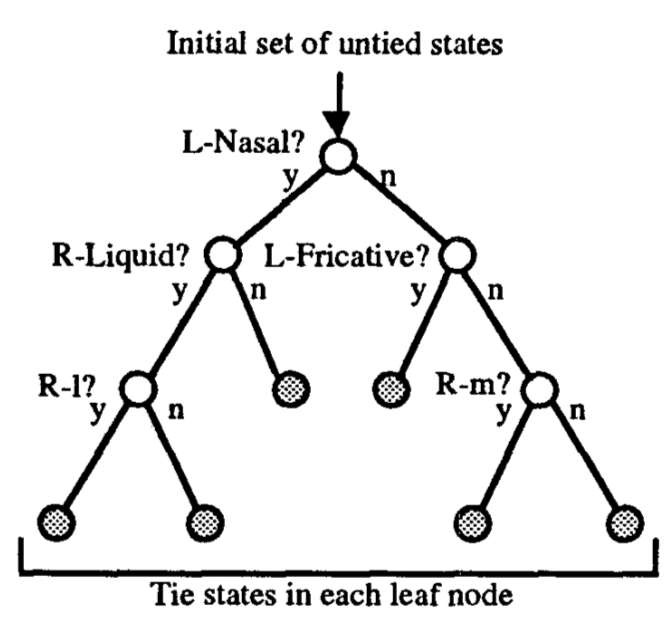
\includegraphics[width=.66\linewidth]{gfx/decision-tree.png}}
        \caption{Phonetic decision tree for HMM state tying \citep{Young1994}.}
        \label{fig:decision-tree}
\end{figure}

The tree input is each triphone being analysed.

The clustering procedures begins by placing all observations in a single root node. All questions are 
analised and the one which maximise the likelihood of a single diagonal
covariance Gaussian is chosen, then the node is split and child nodes generated. The splitting goes on
until it falls below a threshold. Commonly, a minimum threshold is also set, the usual approach is to consider
the frequency of occurence of the phones in a corpus. That it, if a given phone $p$ has $m$ samples and the minimum
threshold is $m$, such that $m>n$, the phone $p$ is mapped unto a more general and robust phone. Consider
that the triphone \textipa{[I-N+g]} appeared 30 times on corpus, and the minimum threshold for splitting the node
was $45$, then \textipa{[I-N+g]} would be modeled into a more general phone, say, for instance, [\textipa{i-N+g}] or 
[\textipa{i-N}].

In the example shown in \autoref{fig:decision-tree}, the first node 
(the root of the tree) checks if the left part of the triphone contains a nasal consonant. If positive, the tree 
examines the right side of the triphone, by questioning
whether it is a liquid consonant. If negative, a leaf is reached and the HMM state to be tied is outputted, e.g. ``tie
the 1\textsuperscript{st} emitting HMM state of the analysed triphone $A$ to [Nasal-$A$+*]''. 
\autoref{fig:state-tying-tree} summarizes the state tying procedure.

\begin{figure}[!htb]
        \myfloatalign
        {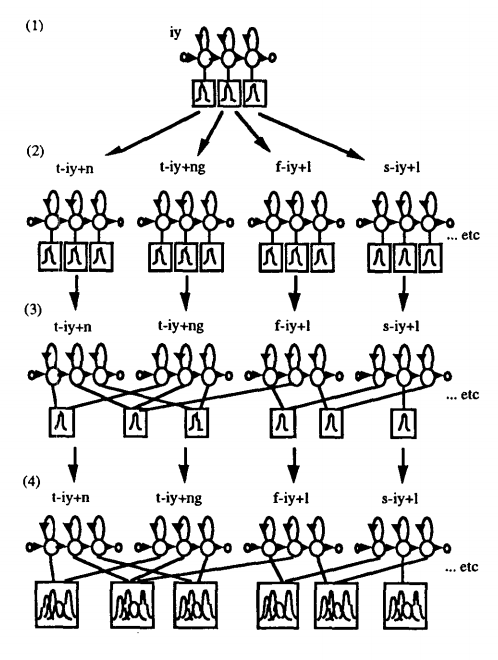
\includegraphics[width=.66\linewidth]{gfx/state-tying-tree.png}}
        \caption{Tied-state HMM system build procedure \citep{Young1994}.}
        \label{fig:state-tying-tree}
\end{figure}

For building the phonetic decision tree for Listener, we based ourselves on the distinctive feature set proposed by 
\citeauthor{Jensen2004} \citep{Jensen2004}, which follows the main guidelines of generative phonology by dividing
the features into four central classes: i) major class features, ii) manner features; iii) place features; and 
iv) laryngeal features.

In practice, classes work as following. Major class features distinguish among the most general classes of sound, 
i.e. vowels, consonants and glides (or semi-vowels). Manner features determine how sounds are articulated, 
that is do they consist of a stop, a nasal, a fricative, a liquid, a trill or a flap? Place features describe 
where in the mouth sounds are produced, whether in the labial region, the alveolar region, the velar region, etc.
Finally, laryngeal features represent the glottal states of sounds, their basic purpose is to differ voiced 
sounds from unvoiced ones.

\citeauthor{Jensen2004} \citep{Jensen2004} proposes a set of $17$ features to describe most of the world languages.

\begin{enumerate}
 \item \emph{Major class features}: syllabic, consonantal and sonorant;
 \item \emph{Manner features}: continuant, nasal, lateral, strident and delayed release;
 \item \emph{Place features}: anterior, coronal, distributed, high, low, back, round and \ac{ATR}.
 \item \emph{Laryngeal features}: voice and \ac{HSP};
\end{enumerate}

The somewhat reduced set for place features is capable of representing a large amount of places of articulation 
since features which are regularly restricted to vowels (such as high, low, back and round) are also shared 
with consonants. Besides, once features have a binary nature, therefore, in theory, a number $n$ of features is able
to dintinguish up to $2^n$ phones. In \autoref{fig:features-place}, a comparison is shown between place features and their corresponding
regions of articulation. For a full explanation of each feature, please see \citeauthor{Jensen2004} \citep{Jensen2004}.

\begin{figure}[!htb]
        \myfloatalign
        {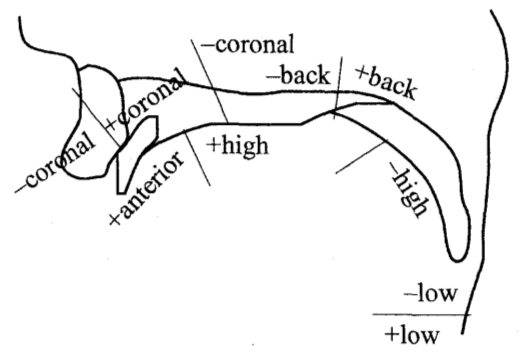
\includegraphics[width=.66\linewidth]{gfx/features-place.png}}
        \caption{Distinctive features for places of places of articulation \citep{Jensen2004}.}
        \label{fig:features-place}
\end{figure}

According to this set of distinctive features, we can arrange the entire phonetic inventory of \ac{AmE} as in \autoref{tab:dist-features-eng}
and that of \ac{BP} as in \autoref{tab:dist-features-bp}.

\tabcolsep=0.15cm
\begin{table}[htbp]
\caption{Distinctive features chart for AmE phones \citep{Jensen2004}.}
\begin{center}
\begin{tabular}{|cc|cccccccccccccccccc|}\hline
 &  & \multicolumn{18}{c|}{\textsc{Distinctive features}} \\ \cline{3-20}
\rotatebox[origin=c]{90}{\textsc{\textsc{CMU symbol}}} & \rotatebox[origin=c]{90}{\textsc{\textsc{IPA symbol}}} & \rotatebox[origin=c]{90}{\textsc{\textsc{syllabic}}} & \rotatebox[origin=c]{90}{\textsc{consonantal}} & \rotatebox[origin=c]{90}{\textsc{sonorant}} & \rotatebox[origin=c]{90}{\textsc{voice}} & \rotatebox[origin=c]{90}{\textsc{HSP}} & \rotatebox[origin=c]{90}{\textsc{continuant}} & \rotatebox[origin=c]{90}{\textsc{nasal}} & \rotatebox[origin=c]{90}{\textsc{lateral}} & \rotatebox[origin=c]{90}{\textsc{strident}} & \rotatebox[origin=c]{90}{\textsc{del. release}} & \rotatebox[origin=c]{90}{\textsc{anterior}} & \rotatebox[origin=c]{90}{\textsc{coronal}} & \rotatebox[origin=c]{90}{\textsc{  distributed  }} & \rotatebox[origin=c]{90}{\textsc{high}} & \rotatebox[origin=c]{90}{\textsc{low}} & \rotatebox[origin=c]{90}{\textsc{back}} & \rotatebox[origin=c]{90}{\textsc{ATR}} & \rotatebox[origin=c]{90}{\textsc{round}} \\ \hline
AA & [\textipa{A}] & + & - & + & + & - & + & - & - & - & - & - & - & - & - & + & + & + & - \\[-3.5pt]
AE & [\textipa{ae}] & + & - & + & + & - & + & - & - & - & - & - & - & - & - & + & - & - & - \\[-3.5pt]
AH & [\textipa{@}] & + & - & + & + & - & + & - & - & - & - & - & - & - & - & - & + & - & - \\[-3.5pt]
AO & [\textipa{O}] & + & - & + & + & - & + & - & - & - & - & - & - & - & - & + & + & - & + \\[-3.5pt]
AW & [\textipa{aU}] & + & - & + & + & - & + & - & - & - & - & - & - & - & - & - & - & - & - \\[-2pt] \hline
AY & [\textipa{aI}] & + & - & + & + & - & + & - & - & - & - & - & - & - & - & - & - & - & - \\[-3.5pt]
B & [\textipa{b}] & - & + & - & + & - & - & - & - & - & - & + & - & - & - & - & - & - & - \\[-3.5pt] 
CH & [\textipa{tS}] & - & + & - & - & - & - & - & - & + & + & - & - & - & - & - & - & - & - \\[-3.5pt] 
D & [\textipa{d}] & - & + & - & + & - & - & - & - & - & - & + & + & - & - & - & - & - & - \\[-3.5pt] 
DH & [\textipa{D}] & - & + & - & + & - & + & - & - & - & - & + & + & - & - & - & - & - & - \\[-2pt] \hline
EH & [\textipa{E}] & + & - & - & + & - & + & - & - & - & - & - & - & - & - & - & - & - & - \\[-3.5pt] 
EY & [\textipa{A\*r}] & + & - & + & + & - & + & - & - & - & - & - & - & - & - & - & - & + & - \\[-3.5pt] 
F & [\textipa{f}] & - & + & - & - & - & + & - & - & - & - & + & - & - & - & - & - & - & - \\[-3.5pt] 
G & [\textipa{g}] & - & + & - & + & - & - & - & - & - & - & - & - & - & - & - & - & - & - \\[-3.5pt] 
HH & [\textipa{h}] & - & + & - & - & - & + & - & - & - & - & - & - & + & - & - & - & - & - \\[-2pt] \hline
IH & [\textipa{I}] & + & - & + & + & - & + & - & - & - & - & - & - & - & + & - & - & - & - \\[-3.5pt] 
IY & [\textipa{i}] & + & - & + & + & - & + & - & - & - & - & - & - & - & + & - & - & + & - \\[-3.5pt] 
JH & [\textipa{dZ}] & - & + & - & + & - & - & - & - & + & + & - & - & - & - & - & - & - & - \\[-3.5pt] 
K & [\textipa{k}] & - & + & - & - & + & - & - & - & - & - & - & - & - & - & - & - & - & - \\[-3.5pt] 
L & [\textipa{l}] & - & + & + & + & - & + & - & + & - & - & + & + & - & - & - & - & - & - \\[-2pt] \hline
M & [\textipa{m}] & - & + & + & + & - & - & + & - & - & - & + & - & - & - & - & - & - & - \\[-3.5pt] 
N & [\textipa{n}] & - & + & + & + & - & - & + & - & - & - & + & + & - & - & - & - & - & - \\[-3.5pt] 
NG & [\textipa{N}] & - & + & + & + & - & - & + & - & - & - & - & - & - & - & - & - & - & - \\[-3.5pt] 
OW & [\textipa{oU}] & + & - & + & + & - & + & - & - & - & - & - & - & - & - & - & + & + & + \\[-3.5pt] 
OY & [\textipa{OI}] & + & - & + & + & - & + & - & - & - & - & - & - & - & - & - & + & - & + \\[-2pt] \hline
P & [\textipa{p}] & - & + & - & - & + & - & - & - & - & - & + & - & - & - & - & - & - & - \\[-3.5pt] 
R & [\textipa{\*r}] & - & + & + & + & - & + & - & - & - & - & + & - & - & - & - & - & - & - \\[-3.5pt] 
S & [\textipa{s}] & - & + & - & - & - & + & - & - & + & - & + & + & - & - & - & - & - & - \\[-3.5pt] 
SH & [\textipa{S}] & - & + & - & - & - & + & - & - & + & - & - & - & + & + & - & - & - & - \\[-3.5pt] 
T & [\textipa{t}] & - & + & - & - & + & - & - & - & - & - & + & + & - & - & - & - & - & - \\[-2pt] \hline
TH & [\textipa{T}] & - & + & - & - & - & + & - & - & - & - & + & + & - & - & - & - & - & - \\[-3.5pt] 
UH & [\textipa{U}] & + & - & + & + & - & + & - & - & - & - & - & - & - & + & - & + & - & + \\[-3.5pt] 
UW & [\textipa{u}] & + & - & + & + & - & + & - & - & - & - & - & - & - & + & - & + & + & + \\[-3.5pt] 
V & [\textipa{v}] & - & + & - & + & - & + & - & - & - & - & + & - & - & - & - & - & - & - \\[-3.5pt] 
W & [\textipa{w}] & - & - & + & + & - & + & - & - & - & - & - & - & - & - & - & - & - & - \\[-2pt] \hline
Y & [\textipa{y}] & - & - & + & + & - & + & - & - & - & - & - & - & - & - & - & - & - & - \\[-3.5pt] 
Z & [\textipa{z}] & - & + & - & + & - & + & - & - & + & - & + & + & - & - & - & - & - & - \\[-3.5pt] 
ZH & [\textipa{Z}] & - & + & - & + & - & - & - & - & + & - & - & - & - & - & - & - & - & - \\ \hline
\end{tabular}
\end{center}
\label{tab:dist-features-eng}
\end{table}


\tabcolsep=0.15cm
\begin{table}[htbp]
\caption{Distinctive features chart for BP phones \citep{Jensen2004}.}
\begin{center}
\begin{tabular}{|cc|cccccccccccccccccc|}\hline
 &  & \multicolumn{18}{c|}{\textsc{Distinctive features}} \\ \cline{3-20}
\rotatebox[origin=c]{90}{\textsc{\textsc{CMU symbol}}} & \rotatebox[origin=c]{90}{\textsc{\textsc{IPA symbol}}} & \rotatebox[origin=c]{90}{\textsc{\textsc{syllabic}}} & \rotatebox[origin=c]{90}{\textsc{consonantal}} & \rotatebox[origin=c]{90}{\textsc{sonorant}} & \rotatebox[origin=c]{90}{\textsc{voice}} & \rotatebox[origin=c]{90}{\textsc{HSP}} & \rotatebox[origin=c]{90}{\textsc{continuant}} & \rotatebox[origin=c]{90}{\textsc{nasal}} & \rotatebox[origin=c]{90}{\textsc{lateral}} & \rotatebox[origin=c]{90}{\textsc{strident}} & \rotatebox[origin=c]{90}{\textsc{del. release}} & \rotatebox[origin=c]{90}{\textsc{anterior}} & \rotatebox[origin=c]{90}{\textsc{coronal}} & \rotatebox[origin=c]{90}{\textsc{  distributed  }} & \rotatebox[origin=c]{90}{\textsc{high}} & \rotatebox[origin=c]{90}{\textsc{low}} & \rotatebox[origin=c]{90}{\textsc{back}} & \rotatebox[origin=c]{90}{\textsc{ATR}} & \rotatebox[origin=c]{90}{\textsc{round}} \\ \hline
a & [\textipa{a}] & + & - & + & + & - & + & - & - & - & - & - & - & - & - & + & + & + & -\\[-4pt]
a$\sim$ & [\textipa{\~a}] & + & - & + & + & - & + & + & - & - & - & - & - & - & - & + & + & + & -\\[-4pt]
b & [\textipa{b}] & - & + & - & + & - & - & - & - & - & - & + & - & - & - & - & - & - & -\\[-4pt]
d & [\textipa{d}] & - & + & - & + & - & - & - & - & - & - & + & + & - & - & - & - & - & -\\[-4pt]
dZ & [\textipa{dZ}] & - & + & - & + & - & - & - & - & + & + & - & - & - & - & - & - & - & -\\[-2pt] \hline
E & [\textipa{E}] & + & - & - & + & - & + & - & - & - & - & - & - & - & - & - & - & - & -\\[-4pt]
e & [\textipa{e}] & + & - & + & + & - & + & - & - & - & - & - & - & - & - & - & - & + & -\\[-4pt]
e$\sim$ & [\textipa{\~e}] & + & - & + & + & - & + & + & - & - & - & - & - & - & - & - & - & + & -\\[-4pt]
f & [\textipa{f}] & - & + & - & - & - & + & - & - & - & - & + & - & - & - & - & - & - & -\\[-4pt]
g & [\textipa{g}] & - & + & - & + & - & - & - & - & - & - & - & - & - & - & - & - & - & -\\[-2pt] \hline
G & [\textipa{G}] & - & + & - & + & - & + & - & - & - & - & - & - & + & - & - & - & + & -\\[-4pt]
i & [\textipa{i}] & + & - & + & + & - & + & - & - & - & - & - & - & - & + & - & - & + & -\\[-4pt]
I & [\textipa{I}] & + & - & + & + & - & + & - & - & - & - & - & - & - & + & - & - & - & -\\[-4pt]
i$\sim$ & [\textipa{\~i}] & + & - & + & + & - & + & + & - & - & - & - & - & - & + & - & - & + & -\\[-4pt]
J & [\textipa{\textltailn}] & - & + & + & + & - & - & + & - & - & - & - & - & + & - & - & - & - & -\\[-2pt] \hline
j & [\textipa{y}] & - & - & + & + & - & + & - & - & - & - & - & - & - & - & - & - & - & -\\[-4pt]
j$\sim$ & [\textipa{\~y}] & - & - & + & + & - & + & + & - & - & - & - & - & - & - & - & - & - & -\\[-4pt]
k & [\textipa{k}] & - & + & - & - & - & - & - & - & - & - & - & - & - & - & - & - & - & -\\[-4pt]
l & [\textipa{l}] & - & + & + & + & - & + & - & + & - & - & + & + & - & - & - & - & - & -\\[-4pt]
L & [\textipa{L}] & - & + & + & + & - & + & - & + & - & - & + & + & + & - & - & - & - & -\\[-2pt] \hline
m & [\textipa{m}] & - & + & + & + & - & - & + & - & - & - & + & - & - & - & - & - & - & -\\[-4pt]
n & [\textipa{n}] & - & + & + & + & - & - & + & - & - & - & + & + & - & - & - & - & - & -\\[-4pt]
O & [\textipa{O}] & + & - & + & + & - & + & - & - & - & - & - & - & - & - & + & + & - & +\\[-4pt]
o & [\textipa{o}] & + & - & + & + & - & + & - & - & - & - & - & - & - & - & - & + & + & +\\[-4pt]
o$\sim$ & [\textipa{\~o}] & + & - & + & + & - & + & + & - & - & - & - & - & - & - & - & + & + & +\\[-2pt] \hline
p & [\textipa{p}] & - & + & - & - & - & - & - & - & - & - & + & - & - & - & - & - & - & -\\[-4pt]
s & [\textipa{s}] & - & + & - & - & - & + & - & - & + & - & + & + & - & - & - & - & - & -\\[-4pt]
S & [\textipa{s}] & - & + & - & - & - & + & - & - & + & - & - & - & + & + & - & - & - & -\\[-4pt]
t & [\textipa{t}] & - & + & - & - & - & - & - & - & - & - & + & + & - & - & - & - & - & -\\[-4pt]
tS & [\textipa{tS}] & - & + & - & - & - & - & - & - & + & + & - & - & - & - & - & - & - & -\\[-2pt] \hline
u & [\textipa{u}] & + & - & + & + & - & + & - & - & - & - & - & - & - & + & - & + & + & +\\[-4pt]
U & [\textipa{U}] & + & - & + & + & - & + & - & - & - & - & - & - & - & + & - & + & - & +\\[-4pt]
u$\sim$ & [\textipa{\~u}] & + & - & + & + & - & + & + & - & - & - & - & - & - & + & - & + & + & +\\[-4pt]
v & [\textipa{v}] & - & + & - & + & - & + & - & - & - & - & + & - & - & - & - & - & - & -\\[-4pt]
w & [\textipa{w}] & - & - & + & + & - & + & - & - & - & - & - & - & - & - & - & - & - & -\\[-2pt] \hline
w$\sim$ & [\textipa{\~w}] & - & - & + & + & - & + & + & - & - & - & - & - & - & - & - & - & - & -\\[-4pt]
x & [\textipa{x}] & - & + & - & - & - & + & - & - & - & - & - & - & + & - & - & - & + & -\\[-4pt]
z & [\textipa{z}] & - & + & - & + & - & + & - & - & + & - & + & + & - & - & - & - & - & -\\[-4pt]
Z & [\textipa{z}] & - & + & - & + & - & - & - & - & + & - & - & - & - & - & - & - & - & -\\[-4pt]
4 & [\textipa{R}] & - & + & + & + & + & + & - & - & - & - & + & - & - & - & - & - & - & -\\[-2pt] \hline
@ & [\textipa{@}] & + & - & + & + & - & + & - & - & - & - & - & - & - & - & + & + & - & -\\ \hline
\end{tabular}
\end{center}
\label{tab:dist-features-bp}
\end{table}

\renewcommand{\arraystretch}{0.55}% Tighter
\tabcolsep=0.15cm
\begin{table}[htbp]
\caption{Distinctive features chart for Listener phones.}
\begin{center}
\begin{tabular}{|ccc|cccccccccccccccccc|}\hline
 & &  & \multicolumn{18}{c|}{\textsc{Distinctive features}} \\ \cline{4-21}
\# & \rotatebox[origin=c]{90}{\textsc{\textsc{Listener symbol}}} & \rotatebox[origin=c]{90}{\textsc{\textsc{IPA symbol}}} & \rotatebox[origin=c]{90}{\textsc{\textsc{syllabic}}} & \rotatebox[origin=c]{90}{\textsc{consonantal}} & \rotatebox[origin=c]{90}{\textsc{sonorant}} & \rotatebox[origin=c]{90}{\textsc{voice}} & \rotatebox[origin=c]{90}{\textsc{HSP}} & \rotatebox[origin=c]{90}{\textsc{continuant}} & \rotatebox[origin=c]{90}{\textsc{nasal}} & \rotatebox[origin=c]{90}{\textsc{lateral}} & \rotatebox[origin=c]{90}{\textsc{strident}} & \rotatebox[origin=c]{90}{\textsc{del. release}} & \rotatebox[origin=c]{90}{\textsc{anterior}} & \rotatebox[origin=c]{90}{\textsc{coronal}} & \rotatebox[origin=c]{90}{\textsc{  distributed  }} & \rotatebox[origin=c]{90}{\textsc{high}} & \rotatebox[origin=c]{90}{\textsc{low}} & \rotatebox[origin=c]{90}{\textsc{back}} & \rotatebox[origin=c]{90}{\textsc{ATR}} & \rotatebox[origin=c]{90}{\textsc{round}} \\ \hline
\footnotesize 1 & \small a & \footnotesize [\textipa{@}] & \footnotesize + & \footnotesize - & \footnotesize + & \footnotesize + & \footnotesize - & \footnotesize + & \footnotesize - & \footnotesize - & \footnotesize - & \footnotesize - & \footnotesize - & \footnotesize - & \footnotesize - & \footnotesize - & \footnotesize + & \footnotesize + & \footnotesize - & \footnotesize -\\ 
\footnotesize 2 & \small aa & \footnotesize [\textipa{A}] & \footnotesize + & \footnotesize - & \footnotesize + & \footnotesize + & \footnotesize - & \footnotesize + & \footnotesize - & \footnotesize - & \footnotesize - & \footnotesize - & \footnotesize - & \footnotesize - & \footnotesize - & \footnotesize - & \footnotesize + & \footnotesize + & \footnotesize + & \footnotesize - \\
\footnotesize 3 & \small aaa & \footnotesize [\textipa{a}] & \footnotesize + & \footnotesize - & \footnotesize + & \footnotesize + & \footnotesize - & \footnotesize + & \footnotesize - & \footnotesize - & \footnotesize - & \footnotesize - & \footnotesize - & \footnotesize - & \footnotesize - & \footnotesize - & \footnotesize + & \footnotesize + & \footnotesize + & \footnotesize -\\
\footnotesize 4 & \small ae & \footnotesize [\textipa{ae}] & \footnotesize + & \footnotesize - & \footnotesize + & \footnotesize + & \footnotesize - & \footnotesize + & \footnotesize - & \footnotesize - & \footnotesize - & \footnotesize - & \footnotesize - & \footnotesize - & \footnotesize - & \footnotesize - & \footnotesize + & \footnotesize - & \footnotesize - & \footnotesize - \\
\footnotesize 5 & \small ah & \footnotesize [\textipa{@}] & \footnotesize + & \footnotesize - & \footnotesize + & \footnotesize + & \footnotesize - & \footnotesize + & \footnotesize - & \footnotesize - & \footnotesize - & \footnotesize - & \footnotesize - & \footnotesize - & \footnotesize - & \footnotesize - & \footnotesize - & \footnotesize + & \footnotesize - & \footnotesize - \\ \hline
\footnotesize 6 & \small am & \footnotesize [\textipa{\~a}] & \footnotesize + & \footnotesize - & \footnotesize + & \footnotesize + & \footnotesize - & \footnotesize + & \footnotesize + & \footnotesize - & \footnotesize - & \footnotesize - & \footnotesize - & \footnotesize - & \footnotesize - & \footnotesize - & \footnotesize + & \footnotesize + & \footnotesize + & \footnotesize -\\
\footnotesize 7 & \small ao & \footnotesize [\textipa{O}] & \footnotesize + & \footnotesize - & \footnotesize + & \footnotesize + & \footnotesize - & \footnotesize + & \footnotesize - & \footnotesize - & \footnotesize - & \footnotesize - & \footnotesize - & \footnotesize - & \footnotesize - & \footnotesize - & \footnotesize + & \footnotesize + & \footnotesize - & \footnotesize + \\
\footnotesize 8 & \small aw & \footnotesize [\textipa{aU}] & \footnotesize + & \footnotesize - & \footnotesize + & \footnotesize + & \footnotesize - & \footnotesize + & \footnotesize - & \footnotesize - & \footnotesize - & \footnotesize - & \footnotesize - & \footnotesize - & \footnotesize - & \footnotesize - & \footnotesize - & \footnotesize - & \footnotesize - & \footnotesize - \\ 
\footnotesize 9 & \small awm & \footnotesize [\textipa{\~w}] & \footnotesize - & \footnotesize - & \footnotesize + & \footnotesize + & \footnotesize - & \footnotesize + & \footnotesize + & \footnotesize - & \footnotesize - & \footnotesize - & \footnotesize - & \footnotesize - & \footnotesize - & \footnotesize - & \footnotesize - & \footnotesize - & \footnotesize - & \footnotesize -\\
\footnotesize 10 & \small ay & \footnotesize [\textipa{aI}] & \footnotesize + & \footnotesize - & \footnotesize + & \footnotesize + & \footnotesize - & \footnotesize + & \footnotesize - & \footnotesize - & \footnotesize - & \footnotesize - & \footnotesize - & \footnotesize - & \footnotesize - & \footnotesize - & \footnotesize - & \footnotesize - & \footnotesize - & \footnotesize - \\  \hline
\footnotesize 11 & \small aym & \footnotesize [\textipa{\~y}] & \footnotesize - & \footnotesize - & \footnotesize + & \footnotesize + & \footnotesize - & \footnotesize + & \footnotesize + & \footnotesize - & \footnotesize - & \footnotesize - & \footnotesize - & \footnotesize - & \footnotesize - & \footnotesize - & \footnotesize - & \footnotesize - & \footnotesize - & \footnotesize -\\
\footnotesize 12 & \small b & \footnotesize [\textipa{b}] & \footnotesize - & \footnotesize + & \footnotesize - & \footnotesize + & \footnotesize - & \footnotesize - & \footnotesize - & \footnotesize - & \footnotesize - & \footnotesize - & \footnotesize + & \footnotesize - & \footnotesize - & \footnotesize - & \footnotesize - & \footnotesize - & \footnotesize - & \footnotesize - \\ 
\footnotesize 13 & \small ch & \footnotesize [\textipa{tS}] & \footnotesize - & \footnotesize + & \footnotesize - & \footnotesize - & \footnotesize - & \footnotesize - & \footnotesize - & \footnotesize - & \footnotesize + & \footnotesize + & \footnotesize - & \footnotesize - & \footnotesize - & \footnotesize - & \footnotesize - & \footnotesize - & \footnotesize - & \footnotesize - \\ 
\footnotesize 15 & \small d & \footnotesize [\textipa{d}] & \footnotesize - & \footnotesize + & \footnotesize - & \footnotesize + & \footnotesize - & \footnotesize - & \footnotesize - & \footnotesize - & \footnotesize - & \footnotesize - & \footnotesize + & \footnotesize + & \footnotesize - & \footnotesize - & \footnotesize - & \footnotesize - & \footnotesize - & \footnotesize -\\  \hline
\footnotesize 16 & \small dh & \footnotesize [\textipa{D}] & \footnotesize - & \footnotesize + & \footnotesize - & \footnotesize + & \footnotesize - & \footnotesize + & \footnotesize - & \footnotesize - & \footnotesize - & \footnotesize - & \footnotesize + & \footnotesize + & \footnotesize - & \footnotesize - & \footnotesize - & \footnotesize - & \footnotesize - & \footnotesize - \\ 
\footnotesize 17 & \small e & \footnotesize [\textipa{e}] & \footnotesize + & \footnotesize - & \footnotesize + & \footnotesize + & \footnotesize - & \footnotesize + & \footnotesize - & \footnotesize - & \footnotesize - & \footnotesize - & \footnotesize - & \footnotesize - & \footnotesize - & \footnotesize - & \footnotesize - & \footnotesize - & \footnotesize + & \footnotesize -\\
\footnotesize 18 & \small eh & \footnotesize [\textipa{E}] & \footnotesize + & \footnotesize - & \footnotesize - & \footnotesize + & \footnotesize - & \footnotesize + & \footnotesize - & \footnotesize - & \footnotesize - & \footnotesize - & \footnotesize - & \footnotesize - & \footnotesize - & \footnotesize - & \footnotesize - & \footnotesize - & \footnotesize - & \footnotesize - \\ 
\footnotesize 19 & \small em & \footnotesize [\textipa{\~e}] & \footnotesize + & \footnotesize - & \footnotesize + & \footnotesize + & \footnotesize - & \footnotesize + & \footnotesize + & \footnotesize - & \footnotesize - & \footnotesize - & \footnotesize - & \footnotesize - & \footnotesize - & \footnotesize - & \footnotesize - & \footnotesize - & \footnotesize + & \footnotesize -\\
\footnotesize 20 & \small ey & \footnotesize [\textipa{A\*r}] & \footnotesize + & \footnotesize - & \footnotesize + & \footnotesize + & \footnotesize - & \footnotesize + & \footnotesize - & \footnotesize - & \footnotesize - & \footnotesize - & \footnotesize - & \footnotesize - & \footnotesize - & \footnotesize - & \footnotesize - & \footnotesize - & \footnotesize + & \footnotesize - \\  \hline
\footnotesize 21 & \small eym & \footnotesize [\textipa{\~y}] & \footnotesize - & \footnotesize - & \footnotesize + & \footnotesize + & \footnotesize - & \footnotesize + & \footnotesize + & \footnotesize - & \footnotesize - & \footnotesize - & \footnotesize - & \footnotesize - & \footnotesize - & \footnotesize - & \footnotesize - & \footnotesize - & \footnotesize - & \footnotesize -\\
\footnotesize 22 & \small f & \footnotesize [\textipa{f}] & \footnotesize - & \footnotesize + & \footnotesize - & \footnotesize - & \footnotesize - & \footnotesize + & \footnotesize - & \footnotesize - & \footnotesize - & \footnotesize - & \footnotesize + & \footnotesize - & \footnotesize - & \footnotesize - & \footnotesize - & \footnotesize - & \footnotesize - & \footnotesize - \\ 
\footnotesize 23 & \small g & \footnotesize [\textipa{g}] & \footnotesize - & \footnotesize + & \footnotesize - & \footnotesize + & \footnotesize - & \footnotesize - & \footnotesize - & \footnotesize - & \footnotesize - & \footnotesize - & \footnotesize - & \footnotesize - & \footnotesize - & \footnotesize - & \footnotesize - & \footnotesize - & \footnotesize - & \footnotesize - \\ 
\footnotesize 24 & \small hh & \footnotesize [\textipa{h}] & \footnotesize - & \footnotesize + & \footnotesize - & \footnotesize - & \footnotesize - & \footnotesize + & \footnotesize - & \footnotesize - & \footnotesize - & \footnotesize - & \footnotesize - & \footnotesize - & \footnotesize + & \footnotesize - & \footnotesize - & \footnotesize - & \footnotesize - & \footnotesize - \\ 
\footnotesize 25 & \small i & \footnotesize [\textipa{i}] & \footnotesize + & \footnotesize - & \footnotesize + & \footnotesize + & \footnotesize - & \footnotesize + & \footnotesize - & \footnotesize - & \footnotesize - & \footnotesize - & \footnotesize - & \footnotesize - & \footnotesize - & \footnotesize + & \footnotesize - & \footnotesize - & \footnotesize + & \footnotesize -\\  \hline
\footnotesize 26 & \small ih & \footnotesize [\textipa{I}] & \footnotesize + & \footnotesize - & \footnotesize + & \footnotesize + & \footnotesize - & \footnotesize + & \footnotesize - & \footnotesize - & \footnotesize - & \footnotesize - & \footnotesize - & \footnotesize - & \footnotesize - & \footnotesize + & \footnotesize - & \footnotesize - & \footnotesize - & \footnotesize - \\ 
\footnotesize 27 & \small im & \footnotesize [\textipa{\~i}] & \footnotesize + & \footnotesize - & \footnotesize + & \footnotesize + & \footnotesize - & \footnotesize + & \footnotesize + & \footnotesize - & \footnotesize - & \footnotesize - & \footnotesize - & \footnotesize - & \footnotesize - & \footnotesize + & \footnotesize - & \footnotesize - & \footnotesize + & \footnotesize -\\
\footnotesize 28 & \small iy & \footnotesize [\textipa{i}] & \footnotesize + & \footnotesize - & \footnotesize + & \footnotesize + & \footnotesize - & \footnotesize + & \footnotesize - & \footnotesize - & \footnotesize - & \footnotesize - & \footnotesize - & \footnotesize - & \footnotesize - & \footnotesize + & \footnotesize - & \footnotesize - & \footnotesize + & \footnotesize - \\ 
\footnotesize 29 & \small jh & \footnotesize [\textipa{dZ}] & \footnotesize - & \footnotesize + & \footnotesize - & \footnotesize + & \footnotesize - & \footnotesize - & \footnotesize - & \footnotesize - & \footnotesize + & \footnotesize + & \footnotesize - & \footnotesize - & \footnotesize - & \footnotesize - & \footnotesize - & \footnotesize - & \footnotesize - & \footnotesize - \\ 
\footnotesize 30 & \small k & \footnotesize [\textipa{k}] & \footnotesize - & \footnotesize + & \footnotesize - & \footnotesize - & \footnotesize + & \footnotesize - & \footnotesize - & \footnotesize - & \footnotesize - & \footnotesize - & \footnotesize - & \footnotesize - & \footnotesize - & \footnotesize - & \footnotesize - & \footnotesize - & \footnotesize - & \footnotesize - \\  \hline
\footnotesize 31 & \small kk & \footnotesize [\textipa{k}] & \footnotesize - & \footnotesize + & \footnotesize - & \footnotesize - & \footnotesize - & \footnotesize - & \footnotesize - & \footnotesize - & \footnotesize - & \footnotesize - & \footnotesize - & \footnotesize - & \footnotesize - & \footnotesize - & \footnotesize - & \footnotesize - & \footnotesize - & \footnotesize -\\
\footnotesize 32 & \small l & \footnotesize [\textipa{l}] & \footnotesize - & \footnotesize + & \footnotesize + & \footnotesize + & \footnotesize - & \footnotesize + & \footnotesize - & \footnotesize + & \footnotesize - & \footnotesize - & \footnotesize + & \footnotesize + & \footnotesize - & \footnotesize - & \footnotesize - & \footnotesize - & \footnotesize - & \footnotesize - \\ 
\footnotesize 33 & \small lh & \footnotesize [\textipa{L}] & \footnotesize - & \footnotesize + & \footnotesize + & \footnotesize + & \footnotesize - & \footnotesize + & \footnotesize - & \footnotesize + & \footnotesize - & \footnotesize - & \footnotesize + & \footnotesize + & \footnotesize + & \footnotesize - & \footnotesize - & \footnotesize - & \footnotesize - & \footnotesize -\\ 
\footnotesize 34 & \small m & \footnotesize [\textipa{m}] & \footnotesize - & \footnotesize + & \footnotesize + & \footnotesize + & \footnotesize - & \footnotesize - & \footnotesize + & \footnotesize - & \footnotesize - & \footnotesize - & \footnotesize + & \footnotesize - & \footnotesize - & \footnotesize - & \footnotesize - & \footnotesize - & \footnotesize - & \footnotesize - \\ 
\footnotesize 35 & \small n & \footnotesize [\textipa{n}] & \footnotesize - & \footnotesize + & \footnotesize + & \footnotesize + & \footnotesize - & \footnotesize - & \footnotesize + & \footnotesize - & \footnotesize - & \footnotesize - & \footnotesize + & \footnotesize + & \footnotesize - & \footnotesize - & \footnotesize - & \footnotesize - & \footnotesize - & \footnotesize - \\  \hline
\footnotesize 36 & \small ng & \footnotesize [\textipa{N}] & \footnotesize - & \footnotesize + & \footnotesize + & \footnotesize + & \footnotesize - & \footnotesize - & \footnotesize + & \footnotesize - & \footnotesize - & \footnotesize - & \footnotesize - & \footnotesize - & \footnotesize - & \footnotesize - & \footnotesize - & \footnotesize - & \footnotesize - & \footnotesize - \\ 
\footnotesize 37 & \small nh & \footnotesize [\textipa{\textltailn}] & \footnotesize - & \footnotesize + & \footnotesize + & \footnotesize + & \footnotesize - & \footnotesize - & \footnotesize + & \footnotesize - & \footnotesize - & \footnotesize - & \footnotesize - & \footnotesize - & \footnotesize + & \footnotesize - & \footnotesize - & \footnotesize - & \footnotesize - & \footnotesize -\\ 
\footnotesize 38 & \small o & \footnotesize [\textipa{o}] & \footnotesize + & \footnotesize - & \footnotesize + & \footnotesize + & \footnotesize - & \footnotesize + & \footnotesize - & \footnotesize - & \footnotesize - & \footnotesize - & \footnotesize - & \footnotesize - & \footnotesize - & \footnotesize - & \footnotesize - & \footnotesize + & \footnotesize + & \footnotesize +\\
\footnotesize 39 & \small om & \footnotesize [\textipa{\~o}] & \footnotesize + & \footnotesize - & \footnotesize + & \footnotesize + & \footnotesize - & \footnotesize + & \footnotesize + & \footnotesize - & \footnotesize - & \footnotesize - & \footnotesize - & \footnotesize - & \footnotesize - & \footnotesize - & \footnotesize - & \footnotesize + & \footnotesize + & \footnotesize +\\ 
\footnotesize 40 & \small ow & \footnotesize [\textipa{oU}] & \footnotesize + & \footnotesize - & \footnotesize + & \footnotesize + & \footnotesize - & \footnotesize + & \footnotesize - & \footnotesize - & \footnotesize - & \footnotesize - & \footnotesize - & \footnotesize - & \footnotesize - & \footnotesize - & \footnotesize - & \footnotesize + & \footnotesize + & \footnotesize + \\  \hline
\footnotesize 41 & \small oy & \footnotesize [\textipa{OI}] & \footnotesize + & \footnotesize - & \footnotesize + & \footnotesize + & \footnotesize - & \footnotesize + & \footnotesize - & \footnotesize - & \footnotesize - & \footnotesize - & \footnotesize - & \footnotesize - & \footnotesize - & \footnotesize - & \footnotesize - & \footnotesize + & \footnotesize - & \footnotesize + \\ 
\footnotesize 42 & \small oym & \footnotesize [\textipa{\~y}] & \footnotesize - & \footnotesize - & \footnotesize + & \footnotesize + & \footnotesize - & \footnotesize + & \footnotesize + & \footnotesize - & \footnotesize - & \footnotesize - & \footnotesize - & \footnotesize - & \footnotesize - & \footnotesize - & \footnotesize - & \footnotesize - & \footnotesize - & \footnotesize -\\
\footnotesize 43 & \small p & \footnotesize [\textipa{p}] & \footnotesize - & \footnotesize + & \footnotesize - & \footnotesize - & \footnotesize + & \footnotesize - & \footnotesize - & \footnotesize - & \footnotesize - & \footnotesize - & \footnotesize + & \footnotesize - & \footnotesize - & \footnotesize - & \footnotesize - & \footnotesize - & \footnotesize - & \footnotesize - \\ 
\footnotesize 44 & \small pp & \footnotesize [\textipa{p}] & \footnotesize - & \footnotesize + & \footnotesize - & \footnotesize - & \footnotesize - & \footnotesize - & \footnotesize - & \footnotesize - & \footnotesize - & \footnotesize - & \footnotesize + & \footnotesize - & \footnotesize - & \footnotesize - & \footnotesize - & \footnotesize - & \footnotesize - & \footnotesize -\\
\footnotesize 45 & \small r & \footnotesize [\textipa{\*r}] & \footnotesize - & \footnotesize + & \footnotesize + & \footnotesize + & \footnotesize - & \footnotesize + & \footnotesize - & \footnotesize - & \footnotesize - & \footnotesize - & \footnotesize + & \footnotesize - & \footnotesize - & \footnotesize - & \footnotesize - & \footnotesize - & \footnotesize - & \footnotesize - \\  \hline
\footnotesize 46 & \small rd & \footnotesize [\textipa{R}] & \footnotesize - & \footnotesize + & \footnotesize + & \footnotesize + & \footnotesize + & \footnotesize + & \footnotesize - & \footnotesize - & \footnotesize - & \footnotesize - & \footnotesize + & \footnotesize - & \footnotesize - & \footnotesize - & \footnotesize - & \footnotesize - & \footnotesize - & \footnotesize -\\ 
\footnotesize 47 & \small s & \footnotesize [\textipa{s}] & \footnotesize - & \footnotesize + & \footnotesize - & \footnotesize - & \footnotesize - & \footnotesize + & \footnotesize - & \footnotesize - & \footnotesize + & \footnotesize - & \footnotesize + & \footnotesize + & \footnotesize - & \footnotesize - & \footnotesize - & \footnotesize - & \footnotesize - & \footnotesize - \\ 
\footnotesize 48 & \small sh & \footnotesize [\textipa{S}] & \footnotesize - & \footnotesize + & \footnotesize - & \footnotesize - & \footnotesize - & \footnotesize + & \footnotesize - & \footnotesize - & \footnotesize + & \footnotesize - & \footnotesize - & \footnotesize - & \footnotesize + & \footnotesize + & \footnotesize - & \footnotesize - & \footnotesize - & \footnotesize - \\ 
\footnotesize 49 & \small t & \footnotesize [\textipa{t}] & \footnotesize - & \footnotesize + & \footnotesize - & \footnotesize - & \footnotesize + & \footnotesize - & \footnotesize - & \footnotesize - & \footnotesize - & \footnotesize - & \footnotesize + & \footnotesize + & \footnotesize - & \footnotesize - & \footnotesize - & \footnotesize - & \footnotesize - & \footnotesize - \\ 
\footnotesize 50 & \small th & \footnotesize [\textipa{T}] & \footnotesize - & \footnotesize + & \footnotesize - & \footnotesize - & \footnotesize - & \footnotesize + & \footnotesize - & \footnotesize - & \footnotesize - & \footnotesize - & \footnotesize + & \footnotesize + & \footnotesize - & \footnotesize - & \footnotesize - & \footnotesize - & \footnotesize - & \footnotesize - \\  \hline
\footnotesize 51 & \small tt & \footnotesize [\textipa{t}] & \footnotesize - & \footnotesize + & \footnotesize - & \footnotesize - & \footnotesize - & \footnotesize - & \footnotesize - & \footnotesize - & \footnotesize - & \footnotesize - & \footnotesize + & \footnotesize + & \footnotesize - & \footnotesize - & \footnotesize - & \footnotesize - & \footnotesize - & \footnotesize -\\
\footnotesize 52 & \small u & \footnotesize [\textipa{u}] & \footnotesize + & \footnotesize - & \footnotesize + & \footnotesize + & \footnotesize - & \footnotesize + & \footnotesize - & \footnotesize - & \footnotesize - & \footnotesize - & \footnotesize - & \footnotesize - & \footnotesize - & \footnotesize + & \footnotesize - & \footnotesize + & \footnotesize + & \footnotesize +\\
\footnotesize 53 & \small uh & \footnotesize [\textipa{U}] & \footnotesize + & \footnotesize - & \footnotesize + & \footnotesize + & \footnotesize - & \footnotesize + & \footnotesize - & \footnotesize - & \footnotesize - & \footnotesize - & \footnotesize - & \footnotesize - & \footnotesize - & \footnotesize + & \footnotesize - & \footnotesize + & \footnotesize - & \footnotesize + \\ 
\footnotesize 54 & \small um & \footnotesize [\textipa{\~u}] & \footnotesize + & \footnotesize - & \footnotesize + & \footnotesize + & \footnotesize - & \footnotesize + & \footnotesize + & \footnotesize - & \footnotesize - & \footnotesize - & \footnotesize - & \footnotesize - & \footnotesize - & \footnotesize + & \footnotesize - & \footnotesize + & \footnotesize + & \footnotesize +\\
\footnotesize 55 & \small uw & \footnotesize [\textipa{u}] & \footnotesize + & \footnotesize - & \footnotesize + & \footnotesize + & \footnotesize - & \footnotesize + & \footnotesize - & \footnotesize - & \footnotesize - & \footnotesize - & \footnotesize - & \footnotesize - & \footnotesize - & \footnotesize + & \footnotesize - & \footnotesize + & \footnotesize + & \footnotesize + \\  \hline
\footnotesize 56 & \small v & \footnotesize [\textipa{v}] & \footnotesize - & \footnotesize + & \footnotesize - & \footnotesize + & \footnotesize - & \footnotesize + & \footnotesize - & \footnotesize - & \footnotesize - & \footnotesize - & \footnotesize + & \footnotesize - & \footnotesize - & \footnotesize - & \footnotesize - & \footnotesize - & \footnotesize - & \footnotesize - \\ 
\footnotesize 57 & \small w & \footnotesize [\textipa{w}] & \footnotesize - & \footnotesize - & \footnotesize + & \footnotesize + & \footnotesize - & \footnotesize + & \footnotesize - & \footnotesize - & \footnotesize - & \footnotesize - & \footnotesize - & \footnotesize - & \footnotesize - & \footnotesize - & \footnotesize - & \footnotesize - & \footnotesize - & \footnotesize - \\ 
\footnotesize 58 & \small y & \footnotesize [\textipa{y}] & \footnotesize - & \footnotesize - & \footnotesize + & \footnotesize + & \footnotesize - & \footnotesize + & \footnotesize - & \footnotesize - & \footnotesize - & \footnotesize - & \footnotesize - & \footnotesize - & \footnotesize - & \footnotesize - & \footnotesize - & \footnotesize - & \footnotesize - & \footnotesize - \\ 
\footnotesize 59 & \small z & \footnotesize [\textipa{z}] & \footnotesize - & \footnotesize + & \footnotesize - & \footnotesize + & \footnotesize - & \footnotesize + & \footnotesize - & \footnotesize - & \footnotesize + & \footnotesize - & \footnotesize + & \footnotesize + & \footnotesize - & \footnotesize - & \footnotesize - & \footnotesize - & \footnotesize - & \footnotesize - \\ 
\footnotesize 60 & \small zh & \footnotesize [\textipa{Z}] & \footnotesize - & \footnotesize + & \footnotesize - & \footnotesize + & \footnotesize - & \footnotesize - & \footnotesize - & \footnotesize - & \footnotesize + & \footnotesize - & \footnotesize - & \footnotesize - & \footnotesize - & \footnotesize - & \footnotesize - & \footnotesize - & \footnotesize - & \footnotesize - \\ \hline
\end{tabular}
\end{center}
\label{tab:dist-features-listener}
\end{table}
\renewcommand{\arraystretch}{1.0}% Normal

\section{Building the Pronunciation Model}

To the best of our knowledge, no previous research has addressed the problem of generating brazilian-accented 
transcriptions for \ac{ASR} purposes or has described the mispronunciations phenomena from a computational perspective. 
Therefore we had to develop our own pronunciation model
\footnote{``Pronunciation models'' are also called ``pronunciation dictionaries''. In this thesis, we are going to
use both terms interchargeably, without any distinction.}. There are basically 
three main approaches we could use to build such model: rule-based methods (XXX CITATION), machine learning methods (XXX CITATION)
and hybrid ones (XXX CITATION). For achieving good performance through machine learning or hybrid approaches, one necessary 
needs a large annotated corpus. That is not the case though. The only Brazilian-accented transcribed corpus we have access
is the Listener Corpus, but we carried out some pilot experiments that showed it was not robust enough for the task.

That being so, we decided to make use of a rule-based approeach for building the pronunciation model. We reviewed all papers 
described in \autoref{ch:second-language}, that deal with the mispronunciation of English phones by brazilians, in order to find 
interlingual allophonies, such as the English [\textipa{T}] usually becomes [\textipa{t}], [\textipa{t\super h}] or [\textipa{f}] in 
beginners' speech \citep{Reis2006}. 

By knowing the allophonies, we developed rules in order to generate the mispronunciations in the dictionary. The mispronunciation contexts
specified through rewrite rules are thus a contribution of this thesis. It is worth mentioning that, for creating the rules, we
took into account the frequency of occurrence of each mispronunciation (when this information was available 
on the papers). On that account mispronunciations which were reported as being very rare or with no significant probability were excluded.

We implemented the rules through a Python script which made a large usage of the \ac{regex} library. As one familiar 
with \ac{regex} knows, \ac{regex} rules might get too clumsy and hard to understand. For instance, one of the rules in our Python script is:

\begin{lstlisting}[float=!h,caption=Example of a fully-specified regex rule.]
re.sub('(ih|iy) (m|n|ng) (#|[^aeiouyw])', r'i~ \3', pron)
\end{lstlisting}

To one not familiar with how the dictionary is structured, this rule, in our opinion, could be somewhat meaningless. Therefore,  to 
render the text easier to read, we are going to describe the rules in a pseudocode with a rather flexible notation
\footnote{For those who are insterested in checking the code itself, it can be downloaded on the site of the project:
\url{http://nilc.icmc.usp.br/listener}}
.
Whenever possible, we try to simplify the rules' contexts, so anyone not acquainted with the dictionary format or the
\ac{regex} syntax might understand their content.

The pseudocode for each mispronunciation pattern is described in the following subsections. The conventions below apply to all examples:

\begin{enumerate}
 \item phonetic transcriptions are placed between brackets and follow the Listener phoneset convention ]
 (see \autoref{sec:listener-phoneset}), therefore [\textipa{"hElow}] becomes [hh eh l ow];
 \item ortographic forms are placed between angle brackets, like <hello>;
 \item the dollar sign ``\$'' represents word final boundary, whether in phonetic or ortographic transcription, 
 thus [ih d\$] means that the transcription ends in [ih d];
 \item the caret symbol ``\textasciicircum'' denotes word initial boundary, whether in phonetic or 
 ortographic transcription, thus <\textasciicircum st> means that word begins with <\textasciicircum st>.
 \item the pipe symbol ``$\vert$'' inside parentheses describes alternatives among a group of phones or 
 graphemes, e.g. [ah (m$\vert$n$\vert$g)] means that [ah] is imediatelly followed by [m], [n] or [ng].
\end{enumerate}

\subsection{Syllable Simplification}
Rules for syllable simplification were created upon production data reported on the following works:
\citeauthor{Cardoso2011} \citep{Cardoso2011}, \citeauthor{Silveira2012} \citep{Silveira2012}
\citeauthor{Rauber2004} \citep{Rauber2004}, and \citeauthor{Rebello2006} \citep{Rebello2006}. The rules
encompass three major cases of syllable simplification. 

The first one refers to stop consonants in word 
final position, such as the final [\textipa{p}] in ``pop'' which is likely to be produced by learners
together with an epenthetic vowel [\textipa{I}], whence [\textipa{"p\super hApI}]. 

The second case regards written language
influencing the learner's pronunciation, e.g. brazilian \ac{ESL} learners tend to pronounce the word ``name'' with a final 
[\textipa{I}], although such vowel does not occur in the English form: [\textipa{"neIm}]. This happens influenced by written language,
in \ac{BP} ortography, a final ``e'' means that the word should end with the phone [\textipa{I}], thus the \ac{ESL} student
transfer put this knowledge into practice in his/her interlanguage. 

The third and last case of syllable simplification concerns initial clusters formed
by [\textipa{s}] and another consonant, hence initial [\textipa{s}C] clusters. In this case, an epenthetic vowel [\textipa{i}] is appended to the
beginning of the word and the consonantal cluster is broken into two syllables, so that [\textipa{s}C] becomes [\textipa{is.}C].

The pseudocode containing rules for all these contexts is defined in \autoref{lst:rules-syll-simplification}.

\lstinputlisting[label=lst:rules-syll-simplification,caption=Pronunciation rules for generating syllable simplification cases.]%
    {Examples/pseudo-rules-syll-simplif.txt}

\subsection{Consonant Change}\label{sec:consonant-change}
The rules for consonantal change were defined based on the results of
\citeauthor{Reis2006} \citep{Reis2006} and \citeauthor{Trevisol2010} \citep{Trevisol2010}.
\autoref{lst:rules-cons-change} describes the pseudecode for generating the mispronunciations regarding consont changes.

\lstinputlisting[float=!htb,label=lst:rules-cons-change,caption=Pronunciation rules for generating consonant change cases.]%
    {Examples/pseudo-rules-cons-change.txt}
    
\subsection{Deaspiration of Voiceless Plosives in Initial or Stressed Positions}

With regard to the deaspiration of voiceless plosives, we considered the analyses of the phenomenon as described in following papers: 
\citeauthor{Alves2008} \citep{Alves2008}, \citeauthor{Prestes2012} \citep{Prestes2012}, 
\citeauthor{Scwartzhaupt2014} \citep{Scwartzhaupt2014} and \citeauthor{Zimmer2006} \citep{Zimmer2006}. These analyses establish 
fundementally the same, brazilian \ac{ESL} learners tend to replace the aspirated phones in English 
[\textipa{p\super h}, \textipa{t\super h}, \textipa{k\super h}] by their corresponding deaspirated ones 
[\textipa{p}, \textipa{t}, \textipa{k}], since the latter ones are part of \ac{BP} phonetic inventory, whereas the former ones are not. 

Therefore, for generating the deaspiration cases, it would simple mean to transform all occurrences of
[\textipa{p\super h}, \textipa{t\super h}, \textipa{k\super h}] into [\textipa{p}, \textipa{t}, \textipa{k}]. However,
in \ac{CMUdict}, the difference aspirated voiceless plosives and the deaspirated ones is not pointed out. Both aspirated and 
non-aspirated plosives are annotated with the same
symbol, for instance, ``pit'' is transcribed as [p ih t] and ``spit'' as [s p ih t], despite the fact that the former [p] is aspirated 
and the latter is not. This is also true for aspirated and non-aspirated [t] and [k]. ``Top'' and ``stop'' are transcribed both with a [t]
although they correspond to different sounds, the same happens with the [k] in ``cat'' and ``scat''.

For solving this problem, we chose to transform all [p, t, k] in the corpus into non-aspirated ones, thus [pp, tt, kk] according
to Listener's phoneset convention (see \autoref{sec:listener-phoneset}. After replacing all [p, t, k] in the dictionary by
[pp, tt, kk], we generated their aspirated counterparts, given that their contexts is predictable. In \ac{AmE}, there basically 
two contexts in which voiceless plosives become aspirated: i) when they occur in a stressed sylllable, not after an [\textipa{s}]; 
ii) and when they occur in word initial position, irrespective of the stress \citep{Lisker1985}. We rewrote these contexts 
into rules, then producing all voiceless aspirated in the corpus.
\footnote{Since deaspiration is also conditioned by the stress of the syllable, we had to move back to the original version of \ac{CMUdict}, 
where lexical stress is annotated. In spite of this, for simplicity we are going to leave this workaround out of the pseudocode 
and assume that the dictionary has the stress information.} The pseudocode for the rules is described in \autoref{lst:rules-deaspiration}.

\lstinputlisting[float=!htb,label=lst:rules-deaspiration,caption=Pronunciation rules for generating plosive deaspiration cases.]%
    {Examples/pseudo-rules-deaspiration.txt}
    
    

\subsection{Devoicing in Word-Final Obstruents}

For terminal devoicing cases, we based our rules on the contexts presented by \citeauthor{Castilho2004} \citep{Castilho2004}.
These rules explicit a phonetic process in which the final [z] becomes devoiced, being produced as [s], in words such as ``Charles'' 
or ``rose''. That is to say these words pronounced as [\textipa{"roUs}] and [\textipa{"tSArls}], instead of [\textipa{"roUz}] 
and [\textipa{"tSArlz}].

\citeauthor{Albuquerque2011} \citep{Albuquerque2011} studied cases of terminal devoicing in plosives, as in [\textipa{"dAg}] 
turning into [\textipa{"dAk}], however their results are inconclusive given the limited sample. 
Besides the study of \citeauthor{Zimmer2012} contradicts \citeauthor{Albuquerque2011} \citep{Albuquerque2011}, for they found 
no statistical significance, in what regards to voicing quality, among the realizations of word final obstruents
between native speakers of English and brazilian \ac{ESL} learners.

For this reason, we decided to discard such phenomenon and deal only with the terminal devoicing of fricatives.
Thereby a more accurate title for this section would be ``devoicing in word-final fricatives'', yet we 
preferred to keep the broader natural class ``obstruents'', since that is how the process is commonly referred to in the literature. 
\autoref{lst:rules-terminal-devoicing} contains the pseudocode for the rewrite rules.
\footnote{It is worth mentioning that the process described in \autoref{sec:consonant-change}, when [\textipa{D}] is realized as
[\textipa{T}] in word-final position is also a case of terminal obstruent devoicing. in spite of this, we did not
find any paper in the literature classifying this phenomenon in such way.}

\lstinputlisting[float=!htb,label=lst:rules-terminal-devoicing,caption=Pronunciation rules for generating terminal devoicing cases.]%
    {Examples/pseudo-rules-obstruent-devoicing.txt}

\subsection{Delateralization and rounding of lateral liquids in final position}
In what concerns to the delateralization and rounding of lateral liquids in final position (also known as vocalization of lateral), we based
our rules in the findings of \citeauthor{Baratieri2006} \citep{Baratieri2006} and \citeauthor{Moore2008} \citep{Moore2008}. Both these authors
describe the same phonetic contexts in which the phenomenon takes place. According to them the English lateral [\textipa{l}] is
pronounced as a vowel [\textipa{U}] by many brazilian \ac{ESL} learners, when such consonant occurs in syllable final position before
a consontar, or in word final position. For instance, learners will tend to say ``salt'' as [\textipa{"kIU}] instead of [\textipa{"kIl}].
The pseudocode with the rules for generating lateral vocalization mispronunciations is found in \autoref{lst:rules-lateral-vocalization}.

\lstinputlisting[float=!htb,label=lst:rules-lateral-vocalization,caption=Pronunciation rules for generating lateral vocalization cases.]%
    {Examples/pseudo-rules-lateral-vocalization.txt}

\subsection{Vocalization of final nasals}

Rules for the vocalization of final nasals were grounded on the phonological processes described in the following works:
\citeauthor{Kluge2007} \citep{Kluge2007}, \citeauthor{Kluge2008} \citep{Kluge2008}, \citeauthor{Kluge2012} \citep{Kluge2012}, 
\citeauthor{Silveira2007} \citep{Silveira2007} and \citeauthor{Silveira2012} \citep{Silveira2012}.
The rules comprise two main cases with respect to the vocalization of final nasals. 

In the first one, the
final nasal is deleted, the previous vowel is nasalized and, if the vowel does not exist in \ac{BP}, it is produced as its
most acoustically similar vowel in \ac{BP}. For instance, in the word ``sandwich'' [\textipa{"s\ae nd.wItS}],
the  [\textipa{\ae n}] is likely
to become [\textipa{\~a}] in the production of brazilian \ac{ESL} learners, with the nasal [\textipa{n}] being deleted, the 
[\textipa{\ae}] vowel being replaced by the \ac{BP} vowel [a] and then becoming nasalized; hence [\textipa{"s\~and.wItS}]. 

The second case addresses L1 spelling patterns interfering in the pronunciation of the brazilian \ac{ESL} learners. This process
is similar to the one described above, the nasal is deleted and the previous is vowel also nasalized, however the vowel quality is 
influenced not perceptual traits, but by the ortographic form of the word. The word ``opium'', for example, although ending
with a schwa [\textipa{@}], [\textipa{"oU.pI.@m}], is usually produced with a [\textipa{\~u}] by the brazilian \ac{ESL} learner, given that an ``u''
appears in the spelling, so [\textipa{"oU.pI.\~u}].

\autoref{lst:rules-nasal-vocalization} contains the pseudocode for generating both cases of final nasal vocalization.

\lstinputlisting[float=!htb,label=lst:rules-nasal-vocalization,caption=Pronunciation rules for generating nasal vocalization cases.]%
    {Examples/pseudo-rules-nasal-vocalization.txt}
    
\subsection{Velar consonantal paragoge}

\lstinputlisting[float=!htb,label=lst:rules-velar-paragoge,caption=Pronunciation rules for generating velar paragoge cases.]%
    {Examples/pseudo-rules-velar-paragoge.txt}

\subsection{Vowel assimilation}

The rules for vowel assimilation were determined based on the results of
\citeauthor{Battistela2010} \citep{Battistela2010}, \citeauthor{Rauber2005} \citep{Rauber2005} and \citeauthor{Rauber2006} \citep{Rauber2006}.
\autoref{lst:rules-vowel-assimilation} contains the pseudecode for generating pronunciations with vowel assimilations from L1 to L2.

\lstinputlisting[float=!htb,label=lst:rules-vowel-assimilation,caption=Pronunciation rules for generating vowel assimilation cases.]%
    {Examples/pseudo-rules-vowel-assimilation.txt}


\subsection{Interconsonantal epenthesis (-ed and -s morphemes)}






%*****************************************
%*****************************************
%*****************************************
%*****************************************
%*****************************************

%*****************************************
\chapter{Results and Discussion}\label{ch:results}
%*****************************************

This is just to test whether this template is working


%*****************************************
%*****************************************
%*****************************************
%*****************************************
%*****************************************

%*****************************************
\chapter{Final Remarks}\label{ch:final-remarks}
%*****************************************


Resultados em reconhecimento de fala, em muitas vezes, s\~ao
explorat\'orios. As l\'inguas s\~ao sistemas din\^amicos, variando dado o
espa\c{c}o, o tempo, os grupos sociais, as situa\c{c}\~oes comunicativas e o
pr\'oprio falante. Tendo em vista que cada l\'ingua possui aspectos
particulares, n\~ao se pode assegurar, no PLN, que m\'etodos j\'a testados
para outros idiomas, sejam diretamente transplantados para o PB e tenham
funcionamento e desempenho similar. Esta disserta\c{c}\~ao busca propor um
m\'etodo de elabora\c{c}\~ao de um sistema de reconhecimento de pron\'uncia para
aprendizes de ingl\^es, falantes nativos do PB. Um sistema desse tipo
ainda n\~ao foi elaborado para o PB e os resultados, portanto, s\~ao
tentativos. Como se discutiu, tal sistema \'e de utilidade, tendo em vista
a baixa profici\^encia em ingl\^es dos brasileiros, demonstrada recentemente
nos \'indices da GlobalEnglish (2012) e da Education First (2013).

A literatura pertinente da \'area foi revisada e m\'etodos que se mostraram
promissores foram selecionados para integrar o projeto. Pretende-se
elaborador um reconhecedor de pron\'uncia que seja capaz de tratar nove
erros de pron\'uncia, provendo feedback ao usu\'ario sobre a qualidade de
sua pron\'uncia. Os erros foram selecionados com base nos trabalhos de
Zimmer (2004), Godoy (2005), Zimmer et al. (2009) e Crist\'ofaro-Silva
(2012), assumindo-se, como pron\'uncia padr\~ao, o General American (GA). A
abordagem de interl\'ingua foi selecionada para a arquitetura do
reconhecedor. O modelo ac\'ustico \'e, assim, alimentado com dados de fala
tanto de nativos, quanto de n\~ao-nativos, aprendizes de ingl\^es. No caso,
para os dados de nativos, ser\'a utilizado o TIMIT; e para os de
n\~ao-nativos, o COBAI e um corpus de leitura de senten\c{c}as foneticamente
balanceadas, ainda a ser compilado. As senten\c{c}as ser\~ao extra\'idas de um
corpus de aprendizes, o COMAprend. Um script em Python ser\'a utilizado
para realizar a convers\~ao grafema-fone das senten\c{c}as, tendo por base a
pron\'uncia can\^onica das palavras registrada no CMU Pronouncing
Dictionary. Na abordagem interlingual, tamb\'em, o modelo de pron\'uncia
deve ser alimentado com as variantes de pron\'uncia do aprendiz, de modo a
compor os chamados dicion\'arios multipron\'uncia. Para isso, pretende-se
utilizar o CMU Pronouncing Dictionary como base e adicionar as hip\'oteses
de pron\'uncia dos aprendizes por meio de regras transformacionais. O
modelo de l\'ingua ser\'a constitu\'ido por trigramas e gerado a partir da
Simple English Wikipedia., de modo a apresentar um sintaxe pr\'oxima à
produ\c{c}\~ao do aprendiz.

Um prot\'otipo foi elaborado de modo a avaliar a viabilidade do m\'etodo ora
proposto. O cronograma de execu\c{c}\~ao do projeto est\'a dentro do prazo, e as
bibliotecas e os softwares necess\'arios para sua execu\c{c}\~ao (HTK, Julius,
Adintool, Audacity, Praat, SoX) j\'a foram testados na elabora\c{c}\~ao do
prot\'otipo. Uma por\c{c}\~ao do COBAI (\textasciitilde{}3h40min) foi
segmentada, alinhada e analisada e utilizada para estimar o modelo
ac\'ustico. Tendo em vista o grande de n\'umero de arquivos do COBAI que
teve de ser desconsiderado (apenas \textasciitilde{}1h30min do que foi
segmentado pode ser utilizado), optou-se por se realizar a coleta de um
corpus de leitura de senten\c{c}as foneticamente balanceadas especificamente
para o desenvolvimento do projeto. De modo a simular, no prot\'otipo, os
dados que se obter\~ao com esse corpus, um corpus de erros induzidos
(\textasciitilde{}2h20min) foi gravado, segmentado, transcrito e
analisado. Tal corpus tamb\'em foi utilizado na estima\c{c}\~ao do modelo
ac\'ustico do prot\'otipo, juntamente com os dados do COBAI. O m\'etodo de
coleta e anota\c{c}\~ao do corpus real, de leitura de senten\c{c}as foneticamente
balanceadas, ser\'a definido em visita t\'ecnica à Universidade de Coimbra,
sob supervis\~ao da Profa. Sara Candeias, no per\'iodo de 28 de janeiro a 28
de fevereiro de 2014. O dicion\'ario-base do modelo de pron\'uncia, o CMU
Pronouncing Dictionary, j\'a foi testado no prot\'otipo, tendo sido
adicionadas variantes de pron\'uncia para um dos erros selecionados: a
simplifica\c{c}\~ao sil\'abica. Foi observado que houve um grande aumento no
n\'umero de entradas no modelo de pron\'uncia com a adi\c{c}\~ao das variantes de
pron\'uncia: o dicion\'ario cresceu de 1.855 palavras para 7.597. Sendo
assim, \'e poss\'ivel, ao se coligir todas as regras para os nove tipos de
erros, que o dicion\'ario cres\c{c}a fortemente, tornando o reconhecimento
confuso, bem como consumindo tempo e recursos computacionais. Caso isso
ocorra, uma solu\c{c}\~ao poss\'ivel seria criar dicion\'arios espec\'ificos para
cada tipo de erro, ou solicitar a um especialista que cerceie o
dicion\'ario, eliminando as variantes que ocorrem com menor frequ\^encia. Os
resultados iniciais obtidos com o prot\'otipo no reconhecimento
mostraram-se promissores.

O conte\'udo do projeto tem sido publicado na web{[}31{]} de modo a
dar-lhe visibilidade e angariar poss\'iveis colaboradores. Pretende-se,
tamb\'em, ao final do projeto, disponibilizar um pequeno sistema de treino
de pron\'uncia, como a prova de conceito para uso do reconhecedor de
pron\'uncia. Uma interface vem sendo desenvolvida para disponibilizar o
prot\'otipo na web, as Figura 19 e Figura 20 trazem algumas telas de
exemplo dessa interface.

                                [pic]

Figura 19: Interface do prot\'otipo na web - vis\~ao geral do site e tela de
captura do \'audio com espectro de frequ\^encia.

\textbar{} {[}i{]} \textbar{} {[}ii{]} \textbar{} \textbar{}{[}pic{]}
\textbar{}{[}pic{]} \textbar{}

Figura 20: Interface do prot\'otipo na web - {[}i{]} palavra reconhecida
com transcri\c{c}\~ao em formato IPA e em alfabeto adaptado; {[}ii{]} tela com
texto de feedback sobre a pron\'uncia do aprendiz, ap\'os ele reiterar no
erro.

H\'a tamb\'em a possibilidade de se realizar visita t\'ecnica ao Laborat\'orio
de Processamento de Sinais (LaPS) da Universidade Federal do Par\'a
(UFPA), na \'epoca de avalia\c{c}\~ao dos resultados finais da disserta\c{c}\~ao, sob
supervis\~ao do Prof.~Aldebaro Klautau, co-orientador da pesquisa.


%\addtocontents{toc}{\protect\clearpage} % <--- just debug stuff, ignore
%\include{multiToC} % <--- just debug stuff, ignore for your documents
% ********************************************************************
% Backmatter
%*******************************************************
\appendix
\part{Appendix}
%********************************************************************
% Appendix
%*******************************************************
% If problems with the headers: get headings in appendix etc. right
%\markboth{\spacedlowsmallcaps{Appendix}}{\spacedlowsmallcaps{Appendix}}
Lorem ipsum at nusquam appellantur his, ut eos erant homero
concludaturque. Albucius appellantur deterruisset id eam, vivendum
partiendo dissentiet ei ius. Vis melius facilisis ea, sea id convenire
referrentur, takimata adolescens ex duo. Ei harum argumentum per. Eam
vidit exerci appetere ad, ut vel zzril intellegam interpretaris.

Errem omnium ea per, pro congue populo ornatus cu, ex qui dicant
nemore melius. No pri diam iriure euismod. Graecis eleifend
appellantur quo id. Id corpora inimicus nam, facer nonummy ne pro,
kasd repudiandae ei mei. Mea menandri mediocrem dissentiet cu, ex
nominati imperdiet nec, sea odio duis vocent ei. Tempor everti
appareat cu ius, ridens audiam an qui, aliquid admodum conceptam ne
qui. Vis ea melius nostrum, mel alienum euripidis eu.

Ei choro aeterno antiopam mea, labitur bonorum pri no. His no decore
nemore graecis. In eos meis nominavi, liber soluta vim cu. Sea commune
suavitate interpretaris eu, vix eu libris efficiantur.

\graffito{More dummy text.}
Nulla fastidii ea ius, exerci suscipit instructior te nam, in ullum
postulant quo. Congue quaestio philosophia his at, sea odio autem
vulputate ex. Cu usu mucius iisque voluptua. Sit maiorum propriae at,
ea cum primis intellegat. Hinc cotidieque reprehendunt eu nec. Autem
timeam deleniti usu id, in nec nibh altera.

Equidem detraxit cu nam, vix eu delenit periculis. Eos ut vero
constituto, no vidit propriae complectitur sea. Diceret nonummy in
has, no qui eligendi recteque consetetur. Mel eu dictas suscipiantur,
et sed placerat oporteat. At ipsum electram mei, ad aeque atomorum
mea.

\begin{table}
    \myfloatalign
  \begin{tabularx}{\textwidth}{Xll} \toprule
    \tableheadline{labitur bonorum pri no} & \tableheadline{que vista}
    & \tableheadline{human} \\ \midrule
    fastidii ea ius & germano &  demonstratea \\
    suscipit instructior & titulo & personas \\
    %postulant quo & westeuropee & sanctificatec \\
    \midrule
    quaestio philosophia & facto & demonstrated \\
    %autem vulputate ex & parola & romanic \\
    %usu mucius iisque & studio & sanctificatef \\
    \bottomrule
  \end{tabularx}
  \caption[Autem usu id]{Autem usu id.}
  \label{tab:moreexample}
\end{table}

Ei solet nemore consectetuer nam. Ad eam porro impetus, te choro omnes
evertitur mel. Molestie conclusionemque vel at, no qui omittam
expetenda efficiendi. Eu quo nobis offendit, verterem scriptorem ne
vix.

  
\begin{lstlisting}[float,caption=A floating example]
for i:=maxint to 0 do
begin
{ do nothing }
end;
\end{lstlisting}
%********************************************************************
% Other Stuff in the Back
%*******************************************************
%********************************************************************
% Bibliography
%*******************************************************
% work-around to have small caps also here in the headline
\manualmark
\markboth{\spacedlowsmallcaps{\bibname}}{\spacedlowsmallcaps{\bibname}} % work-around to have small caps also
%\phantomsection 
\refstepcounter{dummy}
\addtocontents{toc}{\protect\vspace{\beforebibskip}} % to have the bib a bit from the rest in the toc
\addcontentsline{toc}{chapter}{\tocEntry{\bibname}}
\bibliographystyle{plainnat}
\label{app:bibliography} 
\bibliography{Bibliography.bib}
\pagestyle{empty}

\hfill

\vfill


\pdfbookmark[0]{Colophon}{colophon}
\section*{Colophon}
This document was typeset using the typographical look-and-feel \texttt{classicthesis} developed by Andr\'e Miede. 
The style was inspired by Robert Bringhurst's seminal book on typography ``\emph{The Elements of Typographic Style}''. 
\texttt{classicthesis} is available for both \LaTeX\ and \mLyX: 
\begin{center}
\url{http://code.google.com/p/classicthesis/}
\end{center}
Happy users of \texttt{classicthesis} usually send a real postcard to the author, a collection of postcards received so far is featured here: 
\begin{center}
\url{http://postcards.miede.de/}
\end{center}
 
\bigskip

\noindent\finalVersionString

%Hermann Zapf's \emph{Palatino} and \emph{Euler} type faces (Type~1 PostScript fonts \emph{URW
%Palladio L} and \emph{FPL}) are used. The ``typewriter'' text is typeset in \emph{Bera Mono}, 
%originally developed by Bitstream, Inc. as ``Bitstream Vera''. (Type~1 PostScript fonts were made 
%available by Malte Rosenau and
%Ulrich Dirr.)

%\paragraph{note:} The custom size of the textblock was calculated
%using the directions given by Mr. Bringhurst (pages 26--29 and
%175/176). 10~pt Palatino needs  133.21~pt for the string
%``abcdefghijklmnopqrstuvwxyz''. This yields a good line length between
%24--26~pc (288--312~pt). Using a ``\emph{double square textblock}''
%with a 1:2 ratio this results in a textblock of 312:624~pt (which
%includes the headline in this design). A good alternative would be the
%``\emph{golden section textblock}'' with a ratio of 1:1.62, here
%312:505.44~pt. For comparison, \texttt{DIV9} of the \texttt{typearea}
%package results in a line length of 389~pt (32.4~pc), which is by far
%too long. However, this information will only be of interest for
%hardcore pseudo-typographers like me.%
%
%To make your own calculations, use the following commands and look up
%the corresponding lengths in the book:
%\begin{verbatim}
%    \settowidth{\abcd}{abcdefghijklmnopqrstuvwxyz}
%    \the\abcd\ % prints the value of the length
%\end{verbatim}
%Please see the file \texttt{classicthesis.sty} for some precalculated 
%values for Palatino and Minion.
%
%    \settowidth{\abcd}{abcdefghijklmnopqrstuvwxyz}
%    \the\abcd\ % prints the value of the length





%*******************************************************
% Declaration
%*******************************************************
\refstepcounter{dummy}
\pdfbookmark[0]{Declaration}{declaration}
\chapter*{Declaration}
\thispagestyle{empty}
Put your declaration here.
\bigskip
 
\noindent\textit{\myLocation, \myTime}

\smallskip

\begin{flushright}
    \begin{tabular}{m{5cm}}
        \\ \hline
        \centering\myName \\
    \end{tabular}
\end{flushright}

% ********************************************************************
% Game Over: Restore, Restart, or Quit?
%*******************************************************
\end{document}
% ********************************************************************
